% FILE: main.tex  Version 2.1
% AUTHOR:
% Universit�t Duisburg-Essen, Standort Duisburg
% AG Prof. Dr. G�nter T�rner
% Verena Gondek, Andy Braune, Henning Kerstan
% Fachbereich Mathematik
% Lotharstr. 65., 47057 Duisburg
% entstanden im Rahmen des DFG-Projektes DissOnlineTutor
% in Zusammenarbeit mit der
% Humboldt-Universitaet zu Berlin
% AG Elektronisches Publizieren
% Joanna Rycko
% und der
% DNB - Deutsche Nationalbibliothek

% Dies ist die Hauptdatei Ihrer Dissertation. Mit * gekennzeichnete
% Elemente sind optional und k�nnen durch Entfernen/Hinzuf�gen des
% %-Zeichens gew�hlt/abgew�hlt werden. Weitere Informationen
% entnehmen Sie bitte der beiliegenden Brosch�re!
%%%%%%%%%%%%%%%%%%%%%%%%%%%%%%%%%%%%%%%%%%%%%%%%%%%%%%%%%%%%%%%%%%
% Document Class
\RequirePackage[patch]{kvoptions}
\documentclass{dissertation}

%%%%%%%%%%%%%%%%%%%%%%%%%%%%%%%%%%%%%%%%%%%%%%%%%%%%%%%%%%%%%%%%%%
% Packages, Custom Lengths, Environments, and Commands
%% -*- coding: utf-8; -*-
% FILE: command.tex  Version 2.1
% AUTHOR:
% Universität Duisburg-Essen, Standort Duisburg
% AG Prof. Dr. Günter Törner
% Verena Gondek, Andy Braune, Henning Kerstan
% Fachbereich Mathematik
% Lotharstr. 65., 47057 Duisburg
% entstanden im Rahmen des DFG-Projektes DissOnlineTutor
% in Zusammenarbeit mit der
% Humboldt-Universitaet zu Berlin
% AG Elektronisches Publizieren
% Joanna Rycko
% und der
% DNB - Deutsche Nationalbibliothek

%%%%%%%%%%%%%%%%%%%%%%%%%%%%%%%%%%%%%%%%%%%%%%%%%%%%%%%%%%%%%%%%%%
% Packages
\usepackage{algorithm}
\usepackage{algorithmicx}
\usepackage{algpseudocode}
\usepackage{amsmath}
\usepackage{amssymb}
% \usepackage{amsthm}
\usepackage{bm}
\usepackage{booktabs}
\usepackage{breakurl}
\usepackage[font={small,it},justification=centering]{caption}
\usepackage{color}              % \definecolor
\usepackage{colortbl}           % \cellcolor (colored tables)
\usepackage{dirtree}            % \dirtree (draw directory structure)
\usepackage{dsfont}
\usepackage{etoolbox}           % \ifstrempty
\usepackage{epigraph}           % \epigraph
\usepackage{fancyhdr}
\usepackage{footnote}
\usepackage{graphicx}           % \scalebox
\usepackage{hhline}             % \ifstrempty
\usepackage{hyperref}           % clickable table of contents
\usepackage{ifthen}             % \ifthenelse
\usepackage{listings}           % for \lstlisting
\usepackage{mathtools}          % \stackrel, \mathclap
\usepackage{mdframed}           % gray background boxes
\usepackage{multicol}           % for multiple columns in a table
\usepackage{multirow}
\usepackage[authoryear]{natbib}
\usepackage{ntheorem}
\usepackage{paralist}
\usepackage{relsize}
\usepackage{rst}
\usepackage{subcaption}
\usepackage{tabularx}
\usepackage{thmtools}
\usepackage{tikz}
\usepackage[colorinlistoftodos,prependcaption,textsize=tiny]{todonotes}
\usepackage{wasysym}            % smiley symbols
\usepackage{wrapfig}
\usepackage{xcolor}             % \colorlet

\usetikzlibrary{arrows,backgrounds,calc,decorations.markings,%
        positioning,shapes,shapes.misc,snakes}

%%%%%%%%%%%%%%%%%%%%%%%%%%%%%%%%%%%%%%%%%%%%%%%%%%%%%%%%%%%%%%%%%%
%% Lengths
\newlength{\oosixthClmnWidth}
\setlength{\oosixthClmnWidth}{0.055\textwidth}

\newlength{\clmnwidth}
\setlength{\clmnwidth}{0.65\textwidth}
\captionsetup[wraptable]{margin=1cm,width=4cm}

\newlength{\exampleSep}
\setlength{\exampleSep}{0.6em}

%% RST drawing
%% \setlength{\compressionWidth}{100pt}
%% \setlength{\terminalWidth}{0pt}
\setlength{\rstmiddleskip}{1.5em}

\newlength{\hcrfwidth}
\setlength{\hcrfwidth}{0.45\textwidth}
\newlength{\hcrfheight}
\setlength{\hcrfheight}{9em}

%% Epigraph
\setlength\epigraphwidth{.4\textwidth}
\setlength\epigraphrule{0pt}

%%%%%%%%%%%%%%%%%%%%%%%%%%%%%%%%%%%%%%%%%%%%%%%%%%%%%%%%%%%%%%%%%%
%% Colors
\definecolor{chartreuse}{RGB}{127,255,0}
\definecolor{cyan}{rgb}{0.0,0.6,0.6}
\definecolor{darkblue}{rgb}{0.0,0.0,0.6}
\definecolor{darkgoldenrod4}{RGB}{139,101,8}
\definecolor{darkred}{RGB}{139,0,0}
\definecolor{darkslateblue}{RGB}{72,61,139}
\definecolor{deeppink4}{RGB}{139,10,80}
\definecolor{dodgerblue4}{RGB}{16,78,139}
\definecolor{firebrick}{RGB}{178,34,34}
\definecolor{gray69}{RGB}{176,176,176}
\definecolor{gray76}{RGB}{194,194,194}
\definecolor{gray80}{RGB}{204,204,204}
\definecolor{gray84}{RGB}{214,214,214}
\definecolor{gray}{rgb}{0.4,0.4,0.4}
\definecolor{green2}{RGB}{0,238,0}
\definecolor{green3}{RGB}{0,205,0}
\definecolor{green}{RGB}{0,255,0}
\definecolor{highlighter green}{RGB}{27,252,6}
\definecolor{lightcyan4}{RGB}{122,139,139}
\definecolor{midnightblue}{RGB}{25,25,112}
\definecolor{orange3}{RGB}{205,133,0}
\definecolor{red3}{RGB}{205,0,0}
\definecolor{seagreen}{RGB}{46,139,87}
\definecolor{violetred4}{RGB}{139,34,82}

\colorlet{cellcolor}{gray84}

%%%%%%%%%%%%%%%%%%%%%%%%%%%%%%%%%%%%%%%%%%%%%%%%%%%%%%%%%%%%%%%%%%
%% Commands
\newcommand{\vars}{\texttt}
\newcommand{\func}{\textrm}
\newcommand{\ttranslate}[2]{#1

\noindent\emph{#2}}

\renewcommand{\cite}{\citep}
\newcommand{\titlerule}{\rule{0.8\textwidth}{.4pt}}
\providecommand{\shortcite}[1]{\cite{#1}}
\newcommand{\texample}[1]{``\textit{#1}''}
\newcommand{\done}[2][]{\todo[color=green3,#1]{#2}}

\newcommand{\mtag}[3]{{{\upshape[}\ifstrempty{#3}{#2}{\textcolor{#3}{#2}}{\upshape]$_{\textrm{\bfseries\emph{\tiny
          #1}}}$}}}
\newcommand{\sentiment}[2][]{\mtag{sen\-ti\-ment\ifstrempty{#1}{}{:#1}}{#2}{}}
\newcommand{\source}[2][]{\mtag{source\ifstrempty{#1}{}{:#1}}{#2}{darkgoldenrod4}}
\newcommand{\target}[2][]{\mtag{tar\-get\ifstrempty{#1}{}{:#1}}{#2}{darkslateblue}}
\newcommand{\emoexpression}[2][]{\mtag{eex\-pression\ifstrempty{#1}{}{:#1}}{#2}{red}}
\newcommand{\intensifier}[2][]{\mtag{in\-ten\-si\-fier\ifstrempty{#1}{}{:#1}}{#2}{cyan}}
\newcommand{\diminisher}[2][]{\mtag{di\-mi\-ni\-sher\ifstrempty{#1}{}{:#1}}{#2}{}}
\newcommand{\negation}[2][]{\mtag{ne\-ga\-tion\ifstrempty{#1}{}{:#1}}{#2}{deeppink4}}

\newcommand{\argone}[2][]{\mtag{\ifstrempty{#1}{}{rel#1:}arg1}{#2}{darkgoldenrod4}}
\newcommand{\argtwo}[2][]{\mtag{\ifstrempty{#1}{}{rel#1:}arg2}{#2}{darkslateblue}}
\newcommand{\connective}[2][]{\mtag{\ifstrempty{#1}{}{rel#1:}con\-nec\-ti\-ve}{#2}{cyan}}

\newcommand{\argmax}{\operatornamewithlimits{argmax}}
\newcommand{\argmin}{\operatornamewithlimits{argmin}}
\newcommand{\stddev}[1]{{\tiny$^{\pm#1}$}}
\newcommand{\negdelta}[1]{\textsuperscript{\textcolor{red3}{-#1}}}
\newcommand{\posdelta}[1]{\textsuperscript{\textcolor{seagreen}{+#1}}}
\newcommand{\F}[0]{$F_1$}
\newcommand{\NA}{\textcolor{gray69}{NA}}
\newcommand{\expnumber}[2]{{#1}\mathrm{e}^{#2}}
\newcommand{\cev}[1]{\reflectbox{\ensuremath{\vec{\reflectbox{\ensuremath{#1}}}}}}
\newcommand{\norm}[1]{\left\lVert#1\right\rVert}
\newcommand\given[1]{\:#1\vert\:}
\newcommand{\heart}{\ensuremath\heartsuit}
\newcommand{\defeq}{\vcentcolon=}
\newcommand{\eqdef}{=\vcentcolon}
\newcommand{\eg}{\textit{e.g.},}
\newcommand{\ienocomma}{\textit{i.e.}}
\newcommand{\ie}{\ienocomma,}
\newcommand{\corpusDir}{\texttt{PotTS/}}
\newcommand{\nocontentsline}[3]{}
\newcommand{\tocless}[2]{\bgroup\let\addcontentsline=\nocontentsline#1{#2}\egroup}

%% Code Environment
\NewDocumentCommand{\Colorbox}{O{\dimexpr\linewidth-2\fboxsep} m m}{%
  \colorbox{#2}{\makebox[#1][l]{#3}}}
\newcommand{\code}[1]{

\smallskip\noindent\Colorbox{gray80}{\parbox{\textwidth}{\texttt{#1}}}\smallskip

\noindent}

\newcommand{\specialcell}[2][c]{%
  \begin{tabular}[#1]{@{}c@{}}#2\end{tabular}}

\newcommand{\crfEdges}[2]{
    \begin{scope}[on background layer]
      \foreach \prnt in {Neg, Neut, Pos}
        {
           \foreach \chld in {Neg, Neut, Pos}
             \path [-] (#1\prnt) edge node [factor] {} (#2\chld);
        }
    \end{scope}
}

\newcommand{\crfEdgesX}[2]{
    \begin{scope}[on background layer]
      \foreach \prnt in {SNT, TRG, SRC, NON}
        {
           \foreach \chld in {SNT, TRG, SRC, NON}
             \path [-] (\prnt#1) edge node [factor] {} (\chld#2);
        }
    \end{scope}
}

\newcommand{\crfEdgesLatent}[2]{
    \begin{scope}[on background layer]
      \foreach \prnt in {Neg, Neut, Pos}
        {
           \foreach \chld in {Neg, Neut, Pos}
           {
             \path [-,transform canvas={xshift=-1pt}] (#1\prnt) edge node [factor] {} (#2\chld);
             \path [-,transform canvas={xshift=1pt}] (#1\prnt) edge node [factor] {} (#2\chld);
           }
        }
    \end{scope}
}

\newcommand{\crfColoredEdgesLatent}[4]{
    \begin{scope}[on background layer]
      \foreach \prnt in {Neg, Neut, Pos}
        {
           \foreach \chld in {Neg, Neut, Pos}
           {
             \ifthenelse{\(\equal{#1\prnt}{#3} \OR \equal{ANY}{#3}\)  %
                          \AND \(\equal{#2\chld}{#4} \OR \equal{ANY}{#4}\)}{
               \path [-,transform canvas={xshift=-1pt},highlight] (#1\prnt) edge node [factor,highlight] {} (#2\chld);
               \path [-,transform canvas={xshift=1pt},highlight] (#1\prnt) edge node [factor,highlight] {} (#2\chld);
             }{
               \path [-,transform canvas={xshift=-1pt}] (#1\prnt) edge node [factor] {} (#2\chld);
               \path [-,transform canvas={xshift=1pt}] (#1\prnt) edge node [factor] {} (#2\chld);
             }
           }
        }
    \end{scope}
}

%% 3 arguments:
%% Arg1: list of (i, x, w) tuples, where i is the number of feature, x is its x position, and w stands for the feature weight
%% Arg2: index of the parent node
%% Arg3: y position of feature nodes
\newcommand{\crfFeatures}[3]{
    \foreach \i/\x/\w in {#1}
    {
        \node[xnode] (#2FEAT\i) at (\x, #3) {\w};
        \foreach \prnt in {Neg, Neut, Pos}
        {
           \path [-] (#2FEAT\i) edge[] node [factor] {} (#2\prnt);
        }
    }
}

\newcommand{\crfColoredFeatures}[4]{
    \foreach \i/\x/\w in {#1}
    {
        \node[xnode,highlight] (#2FEAT\i) at (\x, #3) {\w};
        \foreach \prnt in {Neg, Neut, Pos}
        {
            \ifthenelse{\equal{\prnt}{#4} \OR \equal{ANY}{#4}}{
              \path [-] (#2FEAT\i) edge[highlight] node [factor,highlight] {} (#2\prnt);
            }{
              \path [-] (#2FEAT\i) edge[] node [factor] {} (#2\prnt);
            }
        }
    }
}

\newcommand{\crfFeaturesX}[3]{
    \foreach \i/\x in {#1}
    {
        \node[xnode] (FEAT\i) at (\x, #3) {};
        \begin{scope}[on background layer]
          \foreach \prnt in {SNT, TRG, SRC, NON}
          {
            \path [-] (FEAT\i) edge node [factor] {} (\prnt#2);
          }
        \end{scope}
    }
}

\newcommand{\crfFeaturesXX}[3]{
    \foreach \i/\x in {#1}
    {
        \node[xnode] (FEAT\i) at (\x, #3) {};
        \begin{scope}[on background layer]
          \foreach \prnt in {SNT, TRG, SRC, DOTS, NON}
          {
            \path [-] (FEAT\i) edge node [factor] {} (\prnt#2);
          }
        \end{scope}
    }
}

\newcommand{\crfFeaturesSemiMarkov}[3]{
    \foreach \i/\x/\d in {#1}
    {
      \node[xnode] (FEAT\i) at (\x, #3) {};
      \begin{scope}[on background layer]
        \foreach \prnt in {SNT, TRG, SRC, NON}
        {
          \path [-] (FEAT\i) edge node [factor] {} (\prnt\d);
        }
      \end{scope}
    }
    \foreach \i/\x/\d in {#2}
    {
      \node[xnode] (FEAT\i) at (\x, #3) {};
      \begin{scope}[on background layer]
        \foreach \prnt in {SNT, TRG, SRC, NON}
        {
          \path [-] (FEAT\i) edge node [factor] {} (\prnt\d);
        }
      \end{scope}
    }
}

%% 3 arguments:
%% Arg1: left node
%% Arg2: middle node
%% Arg3: right node
%% Arg4: hypernode label
\newcommand{\hyperNode}[4]{
    \begin{scope}[on background layer,fill opacity=0.4]
    %% Root
     \filldraw[fill=darkslateblue!45] ($(#1)+(-0.49,0.)$)
        to[out=90,in=180] ($(#2) + (0.,0.47)$)
        to[out=0,in=90] ($(#3) + (0.49,0.)$)
        to[out=270,in=0] ($(#2) + (0.,-0.47)$)
        to[out=180,in=270] ($(#1) + (-0.49,0.)$);
     \node[label] (Root) [above right=0em and 0.3em of #3] {%
                  \textcolor{darkslateblue}{\textsc{\bfseries #4}}};
    \end{scope}
}

\newcommand{\hyperNodeX}[5]{
    \begin{scope}[on background layer,fill opacity=0.4]
    %% Root
     \filldraw[fill=darkslateblue!45] ($(#1)+(0.,0.49)$)
        to[out=0,in=90] ($(#1) + (0.47,0.)$)
        to[out=270,in=90] ($(#2) + (0.47,0.)$)
        to[out=270,in=90] ($(#3) + (0.47,0.)$)
        to[out=270,in=90] ($(#4) + (0.47,0.)$)
        to[out=270,in=0] ($(#4) + (0.,-0.49)$)
        to[out=180,in=270] ($(#4) + (-0.47,0.)$)
        to[out=90,in=270] ($(#3) + (-0.47,0.)$)
        to[out=90,in=270] ($(#2) + (-0.47,0.)$)
        to[out=90,in=270] ($(#1) + (-0.47,0.)$)
        to[out=90,in=180] ($(#1) + (0.,0.49)$);
     \node[label] (Root) [above right=0em and 0.3em of #1] {%
                  \textcolor{darkslateblue}{\textsc{\bfseries #5}}};
    \end{scope}
}

\newcommand{\hyperNodeXX}[6]{
    \begin{scope}[on background layer,fill opacity=0.4]
    %% Root
     \filldraw[fill=darkslateblue!45] ($(#1)+(0.,0.49)$)
        to[out=0,in=90] ($(#1) + (0.87,0.)$)
        to[out=270,in=90] ($(#2) + (0.87,0.)$)
        to[out=270,in=90] ($(#3) + (0.87,0.)$)
        to[out=270,in=90] ($(#4) + (0.87,0.)$)
        to[out=270,in=90] ($(#5) + (0.87,0.)$)
        to[out=270,in=0] ($(#5) + (0,-0.49)$)
        to[out=180,in=270] ($(#5) + (-0.87,0.)$)
        to[out=90,in=270] ($(#4) + (-0.87,0.)$)
        to[out=90,in=270] ($(#3) + (-0.87,0.)$)
        to[out=90,in=270] ($(#2) + (-0.87,0.)$)
        to[out=90,in=270] ($(#1) + (-0.87,0.)$)
        to[out=90,in=180] ($(#1) + (0.,0.49)$);
     \node[label] (Root) [above right=0em and 0.3em of #1] {%
                  \textcolor{darkslateblue}{\textsc{\bfseries #6}}};
    \end{scope}
}

\newcommand{\hyperNodeTreeCRF}[5]{
    \begin{scope}[on background layer,fill opacity=0.4]
    %% Root
     \filldraw[fill=darkslateblue!45] ($(#1)+(-0.49,0.)$)
        to[out=90,in=180] ($(#2) + (0.,0.47)$)
        to[out=0,in=180] ($(#3) + (0.,0.47)$)
        to[out=0,in=90] ($(#4) + (0.49,0.)$)
        to[out=270,in=0] ($(#3) + (0.,-0.47)$)
        to[out=180,in=0] ($(#2) + (0.,-0.47)$)
        to[out=180,in=270] ($(#1) + (-0.49,0.)$);
     \node[label] (Root) [above right=0.3em and 0.em of #4] {%
                  \textcolor{darkslateblue}{\textsc{\bfseries #5}}};
    \end{scope}
}

%% Header, Footer, and Page Layout
\fancyhf{}
\fancyhead[L]{\leftmark}
\rfoot{\thepage}
\pagestyle{fancy}

%% Tikz
\makeatletter
\tikzset{nomorepostaction/.code={\let\tikz@postactions\pgfutil@empty}}
\tikzset{circle split part fill/.style  args={#1,#2}{%
alias=tmp@name, % Jake's idea !!
postaction={%
insert path={
\pgfextra{%
\pgfpointdiff{\pgfpointanchor{\pgf@node@name}{center}}%
{\pgfpointanchor{\pgf@node@name}{east}}%
\pgfmathsetmacro\insiderad{\pgf@x}
%\begin{scope}[on background layer]
%\fill[#1] (\pgf@node@name.base) ([xshift=-\pgflinewidth]\pgf@node@name.east) arc
%                    (0:180:\insiderad-0.5\pgflinewidth)--cycle;
%\fill[#2] (\pgf@node@name.base) ([xshift=\pgflinewidth]\pgf@node@name.west)  arc
%                     (180:360:\insiderad-0.5\pgflinewidth)--cycle;
\fill[#1] (\pgf@node@name.base) ([xshift=-\pgflinewidth]\pgf@node@name.east) arc
(0:180:\insiderad-\pgflinewidth)--cycle;
\fill[#2] (\pgf@node@name.base) ([xshift=\pgflinewidth]\pgf@node@name.west)  arc
(180:360:\insiderad-\pgflinewidth)--cycle;            %  \end{scope}
}}}}}
\makeatother

%% Math
\DeclareMathOperator{\E}{\mathop{\mathbb{E}}}

% Line spacing in matrices
\makeatletter
\renewcommand*\env@matrix[1][\arraystretch]{%
  \edef\arraystretch{#1}%
  \hskip -\arraycolsep
  \let\@ifnextchar\new@ifnextchar
  \array{*\c@MaxMatrixCols c}}
\makeatother

%%%%%%%%%%%%%%%%%%%%%%%%%%%%%%%%%%%%%%%%%%%%%%%%%%%%%%%%%%%%%%%%%%
%% Environments
% uncomment this and the `amsthm` package to get plain uncolored
% examples
% \newtheoremstyle{break}
%   {\topsep}{\topsep}%
%   {\itshape}{}%
%   {\bfseries}{}%
%   {\newline}{}%
% \theoremstyle{break}
% \newtheorem{example}{Example}[section]

\theoremstyle{break}
\theoremheaderfont{\bfseries\upshape}
\newmdtheoremenv[%
linecolor=gray,%
leftmargin=35,%
rightmargin=35,%
backgroundcolor=gray!20,%
innertopmargin=5pt]{example}{Example}[section]

\newtheorem*{Example*}{Example}
% allow fotnotes in tables
\makesavenoteenv{tabular}

%%%%%%%%%%%%%%%%%%%%%%%%%%%%%%%%%%%%%%%%%%%%%%%%%%%%%%%%%%%%%%%%%%
%% Hypersetup
\hypersetup{
    colorlinks=true,
    linktoc=all,
    citecolor=black,
    filecolor=black,
    linkcolor=midnightblue,
    urlcolor=black
}

%%%%%%%%%%%%%%%%%%%%%%%%%%%%%%%%%%%%%%%%%%%%%%%%%%%%%%%%%%%%%%%%%%
%% XML Highlighting
\lstset{
  basicstyle=\tiny,
  columns=fullflexible,
  showstringspaces=false,
  commentstyle=\color{gray}\upshape
}

\lstdefinelanguage{XML}
{
  morestring=[b]",
  morestring=[s]{>}{<},
  morecomment=[s]{<?}{?>},
  stringstyle=\color{black},
  identifierstyle=\color{darkblue},
  keywordstyle=\color{cyan},
  morekeywords={xmlns,id,intensity,mmax_level,span,sarcasm,polarity,version,encoding}%
}


%%%%%%%%%%%%%%%%%%%%%%%%%%%%%%%%%%%%%%%%%%%%%%%%%%%%%%%%%%%%%%%%%%
% Document
\begin{document}

\pagenumbering{roman}
\pagestyle{empty}

% Title Page
% FILE: titlepage.tex  Version 3.0
% AUTHOR:
% Universit�t Duisburg-Essen, Standort Duisburg
% AG Prof. Dr. G�nter T�rner
% Verena Gondek, Andy Braune, Henning Kerstan
% Fachbereich Mathematik
% Lotharstr. 65., 47057 Duisburg
% entstanden im Rahmen des DfG-Projektes DissOnlineTutor
% in Zusammenarbeit mit der
% Humboldt-Universitaet zu Berlin
% AG Elektronisches Publizieren
% Joanna Rycko
% und der
% DNB - Deutsche Nationalbibliothek

%----------Generierung der Titelseite------------------------------------------

\makeatletter % Diese Zeile darf nicht gesl�scht werden!
\title{
\titlerule\\
\Huge \@Title \\
%% \large{\@Subtitle}\\
\titlerule\\
\vspace{0.03\paperheight}
\large\@Fname\ \@Surname\\
\vspace{10em}
\begin{figure*}[htb]
  \centering 
\includegraphics[height=10 em]{img/uni_potsdam.jpg}
\end{figure*}
\vspace{1em}
\large{\textit{\@Type\ eingereicht\\ bei der \@Faculty\\ der \@University}}\\
\vspace{1em}
\the\year
}
\author{}
\date{}

\maketitle

\par\vspace*{\fill}
{
\raggedright
Datum der Einreichung:~\@SubmissionDate \\
\vspace{1cm}
Wissenschaftlicher Betreuer:~\@Supervisor\\
Gutachter: \@GutachterA\\
\vspace{1cm}
Tag der m\"undlichen Pr\"ufung:~\@Pruefungsdatum
}
\makeatother % Diese Zeile darf nicht gel�scht werden!


% Authorship Statement
\vspace*{\fill}

\textit{Ich erkl\"are hiermit, dass die Arbeit selbst\"andig und ohne
  unzul\"assige Hilfe Dritter verfasst wurde und bei der Abfassung nur die in
  der Dissertation angegebenen Hilfsmittel benutzt sowie alle w\"ortlich oder
  inhaltlich \"ubernommenen Stellen als solche gekennzeichnet wurden.}

\begin{flushright}
Potsdam, \the\year

Uladzimir Sidarenka
\end{flushright}
\vspace*{\fill}


% Dedication
% FILE: dedication.tex  Version 2.1
% AUTHOR:
% Universit�t Duisburg-Essen, Standort Duisburg
% AG Prof. Dr. G�nter T�rner
% Verena Gondek, Andy Braune, Henning Kerstan
% Fachbereich Mathematik
% Lotharstr. 65., 47057 Duisburg
% entstanden im Rahmen des DFG-Projektes DissOnlineTutor
% in Zusammenarbeit mit der
% Humboldt-Universitaet zu Berlin
% AG Elektronisches Publizieren
% Joanna Rycko
% und der
% DNB - Deutsche Nationalbibliothek

\thispagestyle{empty}
\vspace*{\fill}
\begin{center}
To my family
\end{center}
\vspace*{\fill}


% Abstract
% FILE: abstract.tex  Version 2.1
% AUTHOR:
% Universit�t Duisburg-Essen, Standort Duisburg
% AG Prof. Dr. G�nter T�rner
% Verena Gondek, Andy Braune, Henning Kerstan
% Fachbereich Mathematik
% Lotharstr. 65., 47057 Duisburg
% entstanden im Rahmen des DFG-Projektes DissOnlineTutor
% in Zusammenarbeit mit der
% Humboldt-Universitaet zu Berlin
% AG Elektronisches Publizieren
% Joanna Rycko
% und der
% DNB - Deutsche Nationalbibliothek
%% \begin{abstract}
%% Here is the english abstract.
%% \end{abstract}
%-englische-Zusammenfassung---------------------------------------
\selectlanguage{english}
\section*{Abstract}
\addcontentsline{toc}{section}{Abstract}

The growing popularity of online conversation platforms over the last few
years has lead to a dramatic increase in the amount of unstructured text data
communicated through these platforms.  As a consequence, dealing with this
abundance of texts in manual way becomes fairly impossible nowadays.  But,
unfortunately, existing automatic natural language processing (NLP) tools --
most of which were created for standard language texts -- cannot handle the
relatively peculiar genre of casual online conversations sufficiently good
either.  Therefore, we urgently need other, more robust and more high-quality
NLP applications which are able to process even such ``unconventional''
linguistic variants as the Web language.  But in order to build them, we first
need to understand the nature of these variants better.

%% But in order to build a high-quality NLP application for a particular language
%% form, one should first understand the nature of this

%% This thesis presents a linguistic and computational study of one of the most
%% proliferating variants of the German online language -- namely, users'
%% microblogs (tweets) posted on Twitter.\footnote{\url{https://twitter.com/}}
%% From the linguistic perspective, we investigate in our work what language
%% phenomena actually account for the notorious language style of tweets making
%% it different from the standard German variant, how frequent those phenomena
%% are,

In this thesis, we present a study of one of the most proliferating forms of
the German online language -- namely, users' conversations on the Twitter
platform.\footnote{\url{https://twitter.com/}} We investigate the specific
characteristics of Twitter messages (tweets) from both linguistic and
computational sides.  From the linguistic perspective, we analyze which
language phenomena actually account for the notoriously peculiar style of
tweets, how frequent those phenomena are and what role they play in the online
communication.  From the computational point of view, we evaluate to what
extent differences in the language style can affect the performance of the
existing NLP approaches and what techniques could help improve this
performance in future.

We conduct our study on three different levels of analysis granularity:
\begin{inparaenum}[\itshape a\upshape)]
    \item the \emph{subsentential},
    \item the \emph{sentential}, and
    \item the \emph{suprasentential} one.
\end{inparaenum}

In the first (\emph{subsentential}) stage of our research, we investigate how
difficult the task of automatic low-level segmentation (i.e. automatic
detection of word and sentence boundaries) is for tweets.  After that, we turn
to the analysis of spelling deviations which are knowingly ubiquituous in
Twitter messages.  In order to estimate how aggravated this problem is, we
collect statistics of the most frequent out-of-vocabulary words drawn from a
sample of users' messages; classify these words into three major classes
(regular German words omitted from dictionaries, stylistic specifics of text
genre, and true spelling deviations), and calculate how frequent each of these
classes are.  We then present possible strategies for handling the latter two
groups (rule-based normalization of stylistic specifics and hybrid correction
of spelling mistakes).  In the description of the related work, we also
juxtapose two general approaches to handling noisy texts -- text normalization
and domain adaptation -- and analyze the pros and cons of these approaches.

On the \emph{sentential} level, we concentrate on the task of automatic
sentiment analysis in sentences.  Here, we first present a comprehensive
corpus of German tweets which were manually annotated with fine-grained
sentiment relations.  We then conduct an agreement study of this corpus in
order to evaluate how difficult the sentiment analysis task is for humans and
which sentiment elements, text topics, and tweet types are most difficult to
annotate.  After that, we demonstrate how well the sentiment classification
task can be done automatically using machine learning and lexicon-based
techniques.  In our experiments, we consider three related subtasks:
\begin{inparaenum}[\itshape a\upshape)]
 \item automatic classification of polar words,
 \item automatic detection of sentiment constituents (i.e. opinion holders,
 targets, and evaluation spans), and, finally,
 \item automatic prediction of the intensity and polarity of sentiments.
\end{inparaenum}

On the \emph{suprasentential} or \emph{discourse} level of the analysis, we
focus our attention on the task of automatic discourse segmentation and
relation extraction.  We first try to apply the ideas of the classical
Rhetorical Structure Theory \citep{Mann-88} to Twitter conversations.  Since
this theory, however, was primarily developed for official monologue texts
rather than casual multilogues, several refinements and extensions to this
framework turned out to be necessary for analyzing Twitter discourses.  These
refinements primarily concern the definition of elementary discourse units
(EDUs) for such Twitter-specific elements as @-mentions, hyperlinks, hashtags
etc.  Furthermore, as we show, several additions to the discourse relations
set are needed in order to cover the interplay between discourse segments both
within and across the tweets.  After defining these extensions, we evaluate
different methods and strategies for automatically detecting EDU boundaries
and discourse structures in microblogs.

In a concluding step, we investigate how using text normalization, on the one
hand, and incorporating discourse information, on the other hand, can help us
improve the results of sentence-level sentiment analysis.


% Acknowledgement
% FILE: acknowledgement.tex  Version 2.1
% AUTHOR:
% Universit�t Duisburg-Essen, Standort Duisburg
% AG Prof. Dr. G�nter T�rner
% Verena Gondek, Andy Braune, Henning Kerstan
% Fachbereich Mathematik
% Lotharstr. 65., 47057 Duisburg
% entstanden im Rahmen des DFG-Projektes DissOnlineTutor
% in Zusammenarbeit mit der
% Humboldt-Universitaet zu Berlin
% AG Elektronisches Publizieren
% Joanna Rycko
% und der
% DNB - Deutsche Nationalbibliothek

\textbf{Acknowledgment.}

At the beginning of this thesis, I would like to say a really big
thank you to all people who supported me throughout these difficult
yet immensely enjoyable years of work on my dissertation; to people
who always were there, when I needed them; to people who taught,
advised, and helped me with my research and who, I believe, made me
stronger, more clever, and perhaps also more confident in my
knowledge.  These people are my colleagues, my friends, my teachers,
but, first of all, my family and my advisor.  I am heavily indebted to
all of them and I am absolutely convinced that this work had never
come into existence if I did not have such a great working environment
as I was lucky to have it in Potsdam.

It would certainly take me another dissertation to express all the
great debt of gratitude that I owe each of my supporters, but I am
afraid they would not accept to wait that long untill I finish it.
So, I should rather try to constrain myself in this acknowledgment and
describe all the infinite gratefulness that I feel for my helpers with
just few but still essential words.

First of all, I certainly would like to thank my advisor, Manfred
Stede, who was much more a ``Doktorvater'' than just a supervisor for
me.  I thank Manfred for his courage in employing me, for the numerous
hours that he invested in our discussions, and for his valuable hints,
suggestions, and criticism.  His experience and wisdom laid the
foundation for the success of this work.  And his patience allowed me
to bring this thesis to the end.  I am very thankful to Manfred that
he introduced me to the amazing world of science, a world which does
not require a visa but which does require a sober mind and a
considerable load of knowledge.  And I sincerely hope that he will
open the doors to this unbelievably beautiful world for many other
Ph.D. students that he certainly will have.

Of course, having a good ``Doktorvater'' is an invaluable precondition
for any completed dissertation, but another prerequisite which plays
an equally important role is still one's own family at home.  And I
have to admit that I had a great luck with both of my families: the
scientific and the traditional one.  My wife and my parents have
always been my greatest supporters.  And, unfortunately, they also
were those people who, I think, suffered most from my absence and the
lack of my spare time.  So, taking this rare opportunity to speak to
them from these pages, I would like to simultaneously apologize for my
possibly neglected family duties and to promise that I will make up
for it in future.

My time at the University of Potsdam had certainly never been that
enjoyable if I did not have such great colleagues as Tatjana
Scheffler, Arne Neumann, Yulia Grishina, Andreas Peldszus, and
Jonathan Sonntag.  I thank Tatjana for her help with our research
project ``Discourse Analysis of Social Media'' and for her valuable
advices and corrections of my papers.  I thank Arne for our talks,
cultural excursions, and his nice attitude to people.  And I am, of
course, much indebted to Yulia who was the most reliable annotator in
our numerous conducted annotation experiments.

I am also especially grateful to our colleagues from the chair of
Theoretical Computational Linguistics -- Alexander Koller and Thomas
Hanneforth.  The unsurpassable level of Alexander's professional
competence and the consummate quality of his work set an example for
me that I eagerly tried to follow.  And even if this humble attempt is
still far away from being completed, it would have been even less
successful if I did not have the unique opportunity to visit Thomas'
fanastic courses in automata theory and C++.  But I am also
particularly thankful to Thomas for the invaluable research hints that
he gave me in our discussions.

Last but not least, I should also mention Konstantina Garoufi, Nikos
Engonopoulos, Mart\'{i}n Villalba, and \v{Z}eljko Agi\'{c} for our
many interesting talks and our enjoyable common lunches.


% Table of Contents, List of Tables and Figures
\setcounter{page}{1}
\tableofcontents
\newpage
\listoffigures
\newpage
\listoftables
\newpage

% Chapters
\pagenumbering{arabic}
\pagestyle{myheadings}

% FILE: introduction.tex  Version 0.01
% AUTHOR: Uladzimir Sidarenka

% This is a modified version of the file main.tex developed by the
% University Duisburg-Essen, Duisburg, AG Prof. Dr. Günter Törner
% Verena Gondek, Andy Braune, Henning Kerstan Fachbereich Mathematik
% Lotharstr. 65., 47057 Duisburg entstanden im Rahmen des
% DFG-Projektes DissOnlineTutor in Zusammenarbeit mit der
% Humboldt-Universitaet zu Berlin AG Elektronisches Publizieren Joanna
% Rycko und der DNB - Deutsche Nationalbibliothek

\chapter{Introduction}

\section{Overview}
As social media become more and more ubiquitous nowadays, the need for
automatic analysis of their data rises.  This analysis, however, is greatly
aggravated by the fact that the language style used on the Web is
fundamentally different from the style that is typical for newspapers or
scientific articles.  Indeed, sentences like the ones shown in Example
\ref{intro:exmp:tweets:en} (taken from \citet{HanBaldwin:11}) are highly
unlikely to appear in editorials or government documents even though their
wording is commonplace on the U.S. English Twitter.
\begin{example}\label{intro:exmp:tweets:en}
u must be talkin bout the paper but I was thinkin movies

\dots so hw many time remaining so I can calculate it?
\end{example}
Similar discrepancies between the formalism of the official style and the
casual nature of spontaneous Web conversations can be observed in other
languages too, and German is not an exception.

It is, however, unclear whether the idiosyncracies of the online style should
be considered as a drawback or an advantage for the automated language
analysis.  While most of the NLP-researchers tend to consider these
peculiarities as a hindrance and even suggest converting online texts to a
more standard language-like form before doing any processing (cf. relevant
works in Section \ref{sec:normalization:relwork}), other scientists at least
object that a straightforward normalization would loose many significant
details and therefore lead to a decrease in the performance.
\citet{BrodyDiakopoulos:11}, for example, claim that the intentional prosodic
lengthenings of the words (like, for example, \texample{sooooooo strong} or
\texample{coooolllllll}) are often a vivid indicator of opinionated sentences
and keeping these elongations in text would result in better sentiment
analysis.  \citet{Collister:11,Collister:12} also notes that the online
discourse deictics like, for instance, \texample{\upshape <--} (the arrow),
\texample{\upshape\^{}} (the carat), and \texample{\upshape *} (the asterisk)
might play an important pragmatic role and this should also be taken into
account when analyzing text.  Furthermore, as noted by \citet{Eisenstein:13},
even in many cases of lexical normalization, changing a colloquial variant of
an expression to its standard language counterpart often involves a
considerable shift in its original meaning.

\paragraph{Goals.}

Providing an answer to the question whether the stylistic peculiarities of the
online language do more harm or good to the automated analysis is precisely
one of the major goals of this dissertation.  We cannot, however, achieve this
goal without realizing first what these stylistic peculiarities in fact are.
That means our first and primary objective is \emph{to find out linguistic
  phenomena that actually account for the idiosyncracies of the Web genre}.

After doing so, the next question that naturally arises is what to do about
these idiosyncrasies -- should we leave them unchanged or should we process
them in some special way and, if so, what this special way might look like?
Thus, the second preliminary objective is \emph{}


Of course, this answer can only be obtained on the basis of empirical results.

can only be
given on the basis of the empirical results.  But before obtaining such
results, one first needs to realize what these peculiarities actually are,
i.e. which linguistic phenomena in fact contribute to the idiosyncracy of the
Web genre.  Finding those phenimena is precisely one of the major goals of
this dissertation.



\paragraph{Goals.}

\paragraph{Research objects.}

But before we start addressing our goals, we first would like to clarify some
methodological aspects that are related to our research.

First of all, we should note that in order to assess the impact of stylistic
peculiarities on the performance of automatic text applications, we need to
answer the question of what these peculiarities actually are, i.e. which
linguistic phenomena in fact contribute to the idiosyncracy of the online
genre.  In order to answer this question, we should conduct an extensive study
of out-of-vocabulary (OOV) words found in Twitter microblogs and divide found
OOVs into separate classes depending on their word formation type.  Then, we
shall investigate which of the suggested classes are typical only for the
online language and which are common for all text genres.

Secondly, after determining the Web-specific elements, we should
\begin{inparaenum}[\itshape a)\upshape]
\item investigate the effect of those elements on the automatic analysis and
\item find an efficient strategy for mitigating the negative consequences of
  that effect.
\end{inparaenum}
For solving the former task, we will compare the performance of the existing
NLP methods obtained on standard language texts with their respective results
achieved on microblog messages.  For solving the latter task, we will first
introduce two general techniques that are commonly used in computational
linguistics for adjusting existing NLP tools to new domains.  These techniques
are called \emph{domain adaptation} and \emph{text normalization}.  We will
briefly describe each of them and shortly point out their strengths and
weaknesses.  After that, we will mainly concentrate on the latter method --
the \emph{text normalization}.

In this task, our goal will be to provide a formal definition of the text
normalization task with regard to Twitter specifics.  As we should see later
and as is also confirmed by \citet{Eisenstein:13}, it will turn out to be
surprisingly difficult to find a precise definition of the normalization.  The
reason for it lies in the fact that the notion of the language ``norm'' by
itself appears to be lax and slippery.

After providing a working definition of normalization, our next goal will be
to investigate different normalization strategies and to find out which of
these strategies are most suitable for treating Twitter-specific phenomena.
This, of course, would not be possible without an appropriate evaluation
metric.  % for measuring how good the performed normalization is.
We will first rely on purely intrisic (\emph{in vitro}) metrics which measure
the normalization quality on its own.

For sure, an in vitro evaluation measure can tell much about the quality of
the performed preprocessing.  But like for many other NLP-related tasks, a
good performance of a standalone module does not necessarily lead to an equal
quality improvement in further downstream processing.  This is especially true
for the text normalization task whose mere positive effect on the subsequent
analysis is often called into question.  \citet{DuBois:07}, for example,
claims that language variation serves a pragmatic and/or stancetaking function
and, consequently, eliminating variation would strip those additional layers
of meaning.  \citet{BrodyDiakopoulos:11} provide a concrete example showing
that intentional prosidic lengthenings of words are often a vivid indicator of
opinionated sentences and keeping these elongations in text would result in
better sentiment analysis.

At this point, we arrive at the third methodological aspect that we need to
address.  Deciding whether Twitter-genre is more or less amenable to automatic
processing and evaluating the effects of text normalization should be done by
inspecting different levels of automatic linguistic analysis.  Because
language is not a uniform object but much more a complex hierarchical
structure, we cannot draw an overall conclusion about its difficulty in
general, if we only inspect one of its multiple levels.  In this work, we
decided to concentrate on three levels:
\begin{inparaenum}[\itshape i)\upshape]
  \item subsentenial (on the example of sentence splitting and tokenization),
  \item sentential (on the example of fine-grained sentiment analysis), and
  \item the suprasentential or discourse level (on the example of discourse
    segmentation and parsing).
\end{inparaenum}

For each of these levels, we will perform automatic analyses of standard
language texts and compare their results with figures obtained on Twitter
corpora.  Since annotated Twitter data are still scarce, we had to develop our
own corpus for each of the above tasks.  In this work, we will briefly discuss
the annotation scheme, the format, the selection criteria and several other
issues involved in the creation of each of these corpora.

Finally, we should note that all evaluations of automatic results should be
done only with respect to the difficulty of that particular tasks for humans.
For this purpose, we will conduct and present extensive inter-annotator
agreement studies for each of our presented corpora and also discuss which
elements, topics, and other linguistic criteria caused most difficulties
during the annotation procedure.  We will then compare the results of the
automatic systems with the results obtained of the inter-annotator agreement
in order to compare how better or worse an automatic system works if compared
to humans.

In the concluding part of our dissertation, we will summarize our results
obtained in each chapter and also investigate how different levels of
automatic analysis might benefit form each other, and how text normalization
procedure affects the final results.

\section{Motivation, Methods, Objects and Goals}
In this work, we should only concentrate on German Twitter.  Though
comparative studies of social media texts in other languages and from other
platforms would certainly be of outermost interest, we only confine ourselves
to this data source, since, in our opinion, any solid comparative research
should first be preceded by thorough studies of the particular domains taken
in isolation and again, in our opinion, little work has been done so far on
German online genre in general and German microblogs in particular.

The motivation for choosing especially Twitter platform is based on the
following factors:
\begin{itemize}
  \item First of all, Twitter data are easy to obtain via public APIs, even
    though they, unfortunately, cannot be distributed in the same
    unproblematic way;
  \item Secondly, the amount of data communicated through this platform is
    growing so rapidly, that the need for the automatic processing of them is
    as urgent as it has never been before for any other kind of social media;
  \item Thirdly, the language of tweets is always at the cutting edge of the
    modern language development.  The free, uncensored way in which people can
    post their information allows for quick responses to any changes in modern
    technology and society.  These changes certainly get reflected in the
    language that people use, and one, of course, could expect that some of
    the changes introduced into the language of the Web might sooner or later
    find their way into the norm of the standard language.  Therefore,
    studying peculiarities of tweets might help us better predict the
    evolution of other linguistic norms;
  \item Fourthly, microblogs renownedly proliferate with various kinds of
    social media-specific phenomena.  Some of these phenomena like, for
    example, @-mentions or \#hashtags are so predominant that they even have
    started penetrating other online platforms like
    Facebook\footnote{\url{https://www.facebook.com/}},
    Instagram\footnote{\url{instagram.com/}},
    Myspace\footnote{\url{https://myspace.com/}} etc.  Therefore, studying
    Twitter might help us better understand peculiarities of other online text
    genres;
  \item Finally, due to a programmatic restriction of the maximal tweet length
    to 140 characters, the concentration of the above mentioned phenomena is
    allegedly one of the highest among all social media types.  Therefore,
    techniques that turn out to bring good results for Twitter might be even
    more efficient for treating data coming from other platforms.
\end{itemize}

The justification for choosing precisely this genre as typical representative
of the ensemble of online languages is given in Section
\ref{sct:intro:twitter}.  The object of our research will be lingustic
differences of Twitter data from the standard language texts and the impact of
these differences on the performace of NLP applications.

\section{Contributions and Outline of this Work}


%% % FILE: chapter-sentiment.tex  Version 0.01
% AUTHOR: Uladzimir Sidarenka

% This is a modified version of the file main.tex developed by the
% University Duisburg-Essen, Duisburg, AG Prof. Dr. G�nter T�rner
% Verena Gondek, Andy Braune, Henning Kerstan Fachbereich Mathematik
% Lotharstr. 65., 47057 Duisburg entstanden im Rahmen des
% DFG-Projektes DissOnlineTutor in Zusammenarbeit mit der
% Humboldt-Universitaet zu Berlin AG Elektronisches Publizieren Joanna
% Rycko und der DNB - Deutsche Nationalbibliothek

\chapter{Text Normalization}\label{chpt:normalization}

\section{Analysis of Out-of-vocabulary Words}

\section{Normalization of Twitter-specific Phenomena}

\section{Normalization of Spelling Deviations}

\section{Evaluation}

\section{Related Work}

\section{Conclusion}


% FILE: chapter-sentiment.tex  Version 0.01
% AUTHOR: Uladzimir Sidarenka

% This is a modified version of the file main.tex developed by the
% University Duisburg-Essen, Duisburg, AG Prof. Dr. G�nter T�rner
% Verena Gondek, Andy Braune, Henning Kerstan Fachbereich Mathematik
% Lotharstr. 65., 47057 Duisburg entstanden im Rahmen des
% DFG-Projektes DissOnlineTutor in Zusammenarbeit mit der
% Humboldt-Universitaet zu Berlin AG Elektronisches Publizieren Joanna
% Rycko und der DNB - Deutsche Nationalbibliothek

\chapter{Text Normalization}

\section{Analysis of Out-of-vocabulary Words}

\section{Normalization of Twitter-specific Phenomena}

\section{Normalization of Spelling Deviations}

\section{Evaluation}

\section{Related Work}

\section{Conclusion}


% FILE: sentiment.tex  Version 0.0.1
% AUTHOR: Uladzimir Sidarenka

% This is a modified version of the file main.tex developed by the
% University Duisburg-Essen, Duisburg, AG Prof. Dr. G�nter T�rner
% Verena Gondek, Andy Braune, Henning Kerstan Fachbereich Mathematik
% Lotharstr. 65., 47057 Duisburg entstanden im Rahmen des
% DFG-Projektes DissOnlineTutor in Zusammenarbeit mit der
% Humboldt-Universitaet zu Berlin AG Elektronisches Publizieren Joanna
% Rycko und der DNB - Deutsche Nationalbibliothek

% FILE: sentiment.tex  Version 0.0.1
% AUTHOR: Uladzimir Sidarenka

% This is a modified version of the file main.tex developed by the
% University Duisburg-Essen, Duisburg, AG Prof. Dr. Günter Törner
% Verena Gondek, Andy Braune, Henning Kerstan Fachbereich Mathematik
% Lotharstr. 65., 47057 Duisburg entstanden im Rahmen des
% DFG-Projektes DissOnlineTutor in Zusammenarbeit mit der
% Humboldt-Universitaet zu Berlin AG Elektronisches Publizieren Joanna
% Rycko und der DNB - Deutsche Nationalbibliothek

% \part{Sentiment Analysis}

\chapter{Introduction to Sentiment Analysis}\label{chap:introduction}

Interpersonal communication is not only a way to share objective
information with other people but also a vibrant channel to convey
one's subjective feelings, impressions, and attitudes.  It is, in
fact, this latter use that provides a personal touch to our
conversations, making them more grasping, more entertaining, and more
living.  And it is often this use that significantly influences our
decisions, preferences, and choices in everyday life.  Therefore, a
high-quality automatic analysis of people's emotions is usually as
important as mining and analysis of objective facts.

The field of knowledge which deals with the analysis of people's
opinions, sentiments, evaluations, appraisals, attitudes, and emotions
towards particular entities mentioned in discourse is called
\emph{sentiment analysis} (SA) \citep{Liu:12}.  The definition of this
discipline, however, much like the definition of the term
\emph{sentiment} itself, is neither complete nor universally accepted.
The main reasons for this are
\begin{inparaenum}[(i)]
  \item a frequently unclear delimitation of the subjective and
    objective components of information and
  \item the heterogeneity of the language system to which SA methods
    are applied.
\end{inparaenum}

The former factor, for instance, makes it difficult to delimitate what
kinds of events and expressions should actually belong to the domain
of sentiment analysis, and which ones shall rather be excluded from
it.  A prominent example of such problematic borderline cases are the
so-called subjective facts, such as ``terrorist attacks'' or ``cancer
drugs,'' which some people perceive as emotionally laden terms while
others regard them as purely objective statements.

The latter factor complicates a precise definition of SA because
different levels of the language have their own concepts of
subjectivity, which in turn require different approaches and methods
to use.  Depending on the language level being analyzed, researchers
typically distinguish three different subtypes of sentiment analysis:
\begin{itemize}
  \item\emph{subsentential} or \emph{fine-grained} SA, whose task is
    to determine and analyze specific subjective opinions and/or
    evaluations within single clauses,
  \item\emph{sentential} analysis, which tries to ascribe a single
    polarity class to each sentence in a text, and
  \item\emph{suprasentential} or \emph{document-level} sentiment
    classification, which seeks to determine the polarity and
    subjectivity classes of complete discourses.
\end{itemize}

Each of these subtypes has its own characteristic strengths and
weaknesses.  Due to these crucial disparities between different
variants of sentiment analysis, speaking of the difficulty or easiness
of this task for a specific domain in general is in the same way wrong
as making overall judgments about the amenability of this domain to
the whole natural language processing field: one always has to specify
the precise level of sentiment analysis whose difficulty is being
analyzed just as she has to set apart a particular NLP task in order
to assess its complicatedness.

\section{Prehistory of the Field}

However, before we delve into the odds and ends of contemporary
sentiment analysis, we first would like to make a short digression
into the history of this field in order to understand its modern
trends and theories better.  Like many other subdisciplines of
computational linguistics, opinion mining has emerged from several
other areas of research, including philosophy, psychology, cognitive
sciences, and last but least narratology and linguistics.

In \emph{philosophy}, the questions about the nature of emotions,
their interaction with human consciousness, and their influence on
people's deeds have occupied the minds of many great scholars,
starting from Plato and Aristotle.  Plato, for instance, argued in his
treatise ``The Republic'' \citep[Book~IV]{Plato:91} that the human
soul presumably consists of three fundamental parts: the rational, the
appetitive, and the passionate.  The last part---the one by which we
become angry or fly into a temper---determines our notion of justice
by favoring either the rational or the appetitive aspect.

These ideas were further particularized and partly revised by Plato's
most prominent student, Aristotle.  In Book~II of ``The Rhetoric''
\citep{Aristotle:54}, Aristotle not only provides a precise taxonomy
and definitions of possible emotions that might constitute the
passionate part of the mind, but also contends that these are both the
reasons for the change of human judgements and the consequences of
those changes \cite[see][p. 157]{Leighton:82}.

As noted by \citet{Sousa:14}, the sheer variety of phenomena covered
by the term ``emotion'' and its closest neighbors tended to discourage
tidy philosophical theories and daunted researchers for a long period
of time.  A real renaissance of emotional studies happened, however,
in the late 19-th century in \emph{psychology} with the introduction
of the James-Lange theory \citep{James:1884}.  In his groundbreaking
work, \citeauthor{James:1884} proclaimed the naturalistic idea that
bodily changes followed directly the perception of the exciting facts,
and that our feelings of the same changes were, in fact, the emotions.
In other words, our biological processes were the primary and the only
reason for us to perceive sentiments.  Independently of James' work,
similar views were proposed by the Danish physician Carl~Lange
\citep{Lange:1885}, who hypothesized that emotional phenomena were the
consequences of cardiovascular events \citep[cf.][]{Lang:94}.

In the 1920s, this theory was severely criticized by Philip~Bard and
Walter~B.~Cannon \citep{Bard:28,Cannon:31}, who proposed an
alternative interpretation of emotions, refuting their connection to
the viscera and arguing that both bodily reactions and subjective
feelings were generated simultaneously in the talamic region of the
brain.  Later on, their conception was in turn put into question by
Stanley Schachter and Jerome E. Singer \citep{Schachter:62}, who
claimed that bodily means alone were insufficient to express the full
range of possible feelings and that cognitive factors could be major
determinants of emotional states. %% To prove this hypothesis, the
%% authors conducted a series of experiments in which they administered
%% epinephrine to human subjects and put them into a room with a
%% specially instructed stooge.  Their study showed that the emotional
%% reaction of the participants crucially depended on the behavior of the
%% stooge during the stay.

These advances in psychology reinforced by the nascent appraisal
theory \citep{Arnold:60} had a significant influence on many other
scientific fields, including but not limited to the \emph{literary
  studies}.  Among the greatest pursuers of this research direction in
narratology, we certainly should name Am\'elie Rorty and Ann Banfield.
\citet{Rorty:80} suggested that the directive power which emotions
exerted over perception was partly a function of their essentially
dramatic or narrative structure \citep[cf.][]{Sousa:14}.
\citet{Banfield:82} investigated how author's and characters'
attitudes could be expressed through direct and indirect speech in
narratives.

One of the first who applied \citeauthor{Banfield:82}'s theory to the
needs and wants of \emph{computational linguistics} was
\citet{Wiebe:90a}.  In her work, the author proposed an algorithm for
identifying characters of narratives whose point of view was being
represented by subjective sentences.  Later on, \citet{Wiebe:94}
further enhanced this system with the possibility to predict
subjective clauses in stories automatically.  This work was allegedly
one of the first experiments on the automatic prediction of sentiments
on the level of single sentences.

The real breakthrough in the sentiment analysis field, however,
happened with the introduction of the first sufficiently big manually
annotated corpora.  Notable contributions in this regard were made by
\citet{Pang:04,Pang:05}, who offered a dataset of $\approx2,000$ movie
reviews with automatically derived polarity classes; \citet{Hu:04},
who presented a manually labeled set of Amazon and C|Net product
feedbacks; \citet{Thomas:06}, who created an automatically labeled
corpus of congressional debates; and, finally, \citet{Wiebe:05}, who
developed a manually annotated sentiment corpus of 535 newspaper
texts.

The availability of these resources has fostered a plethora of new
methods and approaches for both fine- and coarse-grained SA, making
opinion mining one of the most challenging and competitive fields
nowadays.  Important cornerstones in this discipline have already been
established by the works of \citet{Pang:02}, \citet{Wiebe:05},
\citet{Wilson:05}, \citet{Breck:07}, \citet{Choi:09,Choi:10},
\citet{Yessenalina:11}, \citet{Socher:11, Socher:12} and many others.
Nevertheless, many challenges of sentiment analysis, such as domain
adaptation or analysis of non-English texts, still pose considerable
difficulties.

\section{Sentiment Analysis of Social Media}

One of the main problems that people working on opinion mining are
typically confronted with in the first place is that of the discourse
domain to be analyzed.  Since sentiment analysis is a highly
domain-dependent task \citep[cf.][]{Aue:05,Blitzer:07,Li:08} -- \ie{}
systems trained for specific topics and on specific text genres do not
neatly generalize to other subjects and other linguistic styles -- a
natural question that arises in this context is which of the domains
should be addressed first in that case.

While earlier sentiment works were primarily concerned with narratives
\citep{Wiebe:90a,Wiebe:94} or newspaper articles
\citep{Wiebe:03,Wiebe:05,Bautin:08}, it soon became clear that social
media provides a much more fertile ground for mining people's
opinions.  The reason for this is the virtual absence of any
moderation on many modern CMC services.  This lack of censorship
allows users to be upfront about their feelings.  Combined with the
great popularity of social networks, such freedom of expressing one's
thoughts makes social media the arguably most prolific channel for
sharing (and mining) personal emotions.

It is therefore not surprising that the rapid emergence of numerous SM
websites was accompanied by an increasing interest in their content
from many NLP practitioners.  One of the first who attempted to
extract users' evaluations automatically from CMC services were
\citet{Das:01}.  The authors investigated the correlation between
users' attitudes on economic chat boards and stock prices for about
eight stocks.  For this purpose, they trained a collection of five
classifiers on a training set of 500 messages that were manually
labeled with three classes: \emph{buy} (positive evaluations),
\emph{sell} (negative evaluations), and \emph{null} (neutral
statements).  With these classifiers, they subsequently annotated the
rest of the downloaded 25,000 posts, taking the majority votes of the
five systems as the final labels, and then scrutinized the
interrelationship between these predictions and the observed stock
indices.
%% This study revealed that user chats strongly correlated with stock
%% developments in a reactive way: changes in stock prices had
%% typically lead to fluctuations of public opinions but not vica
%% versa.

\citet{Glance:05} also used sentiment analysis for business
intelligence purposes by mining users' opinions on Usenet newsgroups
with a set of hand-crafted rules.  Further notable works in this
direction include those of \citet{Antweiler:04}, who investigated how
postings on stock message boards correlated with stock volatility;
\citet{Gruhl:05}, who studied the cross-correlation between online
mentions of products and sales spikes for that commodities, also
proposing an algorithm for tracking such correlations and making
predictions about products' future sales automatically; finally,
\citet{Ghose:07} examined the effect of opinions on the pricing power
of merchants in online marketplaces, claiming that more positive
opinions on the Web entitled traders to increase their selling prices.

A separate line of research that is closely related to both commercial
intelligence and sentiment analysis of social media involves opinion
mining of product reviews.  A pioneering work in this direction was
done by \citet{Turney:02}, who performed a two-class classification of
410 Epinions comments, dividing customers' reviews of automobiles,
banks, movies, and travel destinations into \emph{recommended} (thumbs
up) and \emph{not recommended} (thumbs down) ones.  In order to make
these decisions, the proposed system first computed the sum of the
pointwise mutual information (PMI) scores between the adjectival and
adverbial phrases occurring in a review text and the word
``excellent,'' and then subtracted from this the PMIs of the found
phrases in conjunction with the word ``poor.''  Reviews with negative
results were subsequently considered as \emph{thumbs down}, and
comments with non-negative total scores were correspondingly
classified as \emph{thumbs up}.

According to \citet{Turney:02}, the most challenging type of reviews
to analyze in these experiments were the movie critiques (the accuracy
on this subset only reached 66\%, whereas, for banks and automobiles,
it attained 80 and 84\% respectively).  This finding was also
confirmed by \citet{Pang:02} who tried out several machine learning
classifiers on a manually annotated corpus of $\approx2,000$ write-ups
from the Internet Movie Database (IMDb).  The best results (82.9\%
accuracy) for the two-class classification task (\emph{positive}
versus \emph{negative}) were attained by an SVM system which used the
presence of unigrams as classification features.

Due to its high commercial impact, opinion mining of customer reviews
soon became one of the most popular topics in sentiment analysis
research.  \citet{Dave:03}, for example, attempted to classify C|Net
and Amazon reviews of movies and electrical appliances as positive or
negative using the Na\"{\i}ve Bayes and SVM approaches.  \citet{Hu:04}
developed a three-stage application which first identified products'
features in reviews, then looked for opinionated words associated with
those features, and, finally, produced concise summaries of positive
and negative opinions about each particular product aspect.
\citet{Funk:08} proposed a supervised SVM-system to perform two- and
five-way polarity classification of product reviews, also using these
predictions in a business intelligence system.  Other important
milestones in this research direction were set by the works of
\citet{Popescu:05}, \citet{Ding:09}, \citet{Wei:10},
\citet{Mukherjee:12}, and many others.

%% The authors found that replacing certain entities, such as product
%% names, abbreviations, or numerals, with special meta-tokens and
%% using token n-grams of different lengths had a significant positive
%% effect on the accuracy of both classifiers.

Notwithstanding that product reviews continued playing a crucial role
for the success of the e-commerce, with the increasing spread of
blogging services and social networks, sentiment researchers have
gradually shifted the focus of their work from product feedbacks to
these upcoming text genres.  \citet{Mishne:05} and \citet{Mishne:07},
for instance, tried to classify Livejournal blogs according to the
moods of their authors (e.g.  \emph{amused}, \emph{tired},
\emph{happy} etc.).  The gold labels for their $\approx$~815,000 blog
corpus were obtained automatically from blog labels on the Livejournal
website.  On this corpus, the authors trained a supervised SVM
classifier, reaching an average of 8\% improvement over the 50\%
baseline.

\citet{Chesley:06} also applied an SVM system in order to classify
user blogs into objective, positive and negative subjective ones.  The
authors derived their features from the Wiktionary and the InfoXtract
lexicon \citep{Srihari:03} and attained an accuracy increase of up to
15~\% over the majority class baseline.  This research direction was
further continued by \citet{Godbole:07}, who applied a lexicon-based
method to detect users' opinions in newspapers and blogs; and
\citet{Gill:08}, who conducted an inter-annotator agreement study of
mood detection in blogs, finding that raters' consensus on the
expressed emotions strongly increased with the length of blog entries.

Speaking of blog length, it should certainly be said that the
inception of the micro-blogging service Twitter in 2006 was a real
game changer to the opinion mining field: the sudden availability of
huge amounts of data; the presence of all possible social, national,
and age groups combined with a high idiosyncrasy and diversity of the
language used on this service gave rise to numerous scientific
projects, studies, and publications, which we will briefly summarize
in the next subsection.

\section{Sentiment Analysis of Twitter}\label{snt:subsec:intro:saot}

Among the first attempts at an automatic sentiment analysis of Twitter
was the study conducted by \citet{Go:09}.  In their experiments, the
authors collected a set of 1,600,000 microblogs containing smileys.
Based on these emoticons, they automatically derived polarity classes
of these tweets (positive or negative) and then used these
bootstrapped labels to train the Na\"{\i}ve Bayes, MaxEnt, and SVM
classifiers.  The last system produced the best results, reaching an
$F$-score of 82.2\%.

A similar approach was also used by \citet{Pak:10}, who applied the
Na\"{\i}ve Bayes method to differentiate between neutral, positive,
and negative messages.  Likewise, \citet{Davidov:10} obtained the gold
labels for their corpus using distant supervision and then trained a
kNN-like classifier on this dataset.

A different way of collecting the data was proposed by
\citet{Barbosa:10}.  The authors gathered a collection of 200,000
microblogs from three publicly available sentiment web-services.
Using the majority votes of these websites as the gold categories for
their tweets, they trained a supervised SVM system on this corpus and
then let this system predict the subjectivity and polarity classes of
new unseen messages.

The emoticon
dataset\footnote{\url{http://twittersentiment.appspot.com}} of
\citet{Go:09} along with a subset of the Edinburgh Twitter corpus
\cite{Petrovic:10} was later used by \citet{Kouloumpis:11}, who
trained an AdaBoost classifier on these data.  Reaching an average
$F1$-measure of 68\% on a held-out manually labeled dataset, the
authors came to the conclusion that microblog-specific features (such
as the presence or absence of intensifiers or the occurrence of
abbreviations and emoticons) were the most reliable traits for this
classification.  This finding, however, was doubted by
\citet{Agarwal:11}, who contended that POS-specific polarity features
and tree-kernel methods were a better alternative.

Similarly to the opinion mining of customer reviews, sentiment
analysis of Twitter could not go unnoticed by the economic and
sociological communities.  One of the first attempts to analyze tweets
from these perspectives was made by \citet{Jansen:09}, who studied
microblogs' power as online word of mouth.  A manual inspection of
messages mentioning renowned company brands revealed that almost 20\%
of these tweets expressed some polar opinions about their products.
More than a half of these opinionated microblogs were positive
judgements, whereas 35\% of the posts represented negative sentiments.
These findings strongly correlated with the results of an automatic
analysis, suggesting that social media in general and microblogging in
particular could be a valuable source of economic evidence.

An attempt to address sociological problems with SA methods was made
by \citet{Tumasjan:10}, who analyzed public opinions about federal
elections in Germany by automatically extracting sentiments from
users' microblogs.\footnote{We will make a similar analysis in Section
  \ref{chap:fgsa} but will primarily concentrate on the NLP aspect of
  this problem.}  For this purpose, the authors had gathered a
collection of nearly 100,000 messages mentioning major political
parties or prominent German politicians and subsequently translated
these tweets into English.  The resulting translations were analyzed
with the proprietary LIWC software \cite{Pannebaker:07}, which used
relative word counts to compute associations between the given topics
and a pre-defined emotions set.  This study also proved that Twitter
could serve as a platform for political deliberation and that the mere
number of tweets referencing some party strongly corresponded to the
results of political election polls.

As in the previous cases, a key factor for the success and popularity
of this subfield among NLP researchers was the creation and
dissemination of high-quality big annotated corpora.  An important
role in this respect was played by the organizers of the SemEval
competition on sentiment analysis in Twitter
\cite{Nakov:13,Rosenthal:14,Rosenthal:15}.

For the first run of the shared task in \citeyear{Nakov:13},
\citet{Nakov:13} prepared a substantially-sized dataset with more than
15,000 messages (the SemEval Tweet corpus), which were manually
labeled on the crowdsourcing platform Amazon Mechanical Turk.  To that
end, five Turkers were asked to determine the overall polarity of each
collected microblog and to annotate all occurrences of subjective
expressions in those messages with their contextual polarity.

The best performing system in the first iteration -- a supervised SVM
classifier of \citet{Mohammad:13} -- won three out of four subtasks.
This solution relied on an extensive set of hand-crafted surface-form,
semantic, and syntactic features and also actively used multiple
manually and automatically generated sentiment lexica, including the
NRC emotion lexicon of \citeauthor{Mohammad:13a}
(\citeyear{Mohammad:13a}), the MPQA lexicon of \citeauthor{Wilson:05}
(\citeyear{Wilson:05}), and the sentiment list of \citeauthor{Hu:04}
(\citeyear{Hu:04}).  The authors noticed a crucial impact of the
lexicon features on the quality of final predictions (an ablation test
showed that the results of the system worsened by $\approx8.5\%$ when
the lexicon information was removed).

Other competing submissions \cite{Becker:13,Guenther:13,Kokciyan:13}
basically utilized the same approach but used considerably less
information from lexicons.  Nevertheless, all 10 top-scoring systems
in this run could correctly predict the phrase-level polarity of
subjective expressions in more than 80\% of the cases and also
outperformed the 60\% benchmark when classifying the overall polarity
of the tweets.

The success of this shared task, which attracted more than 40
participants, incited the organizers to continue this competition in
the following years.  With slight modifications (addition of new
tweets, inclusion of sarcastic microblogs and LiveJournal sentences),
both subtasks were re-offered in \citeyear{Rosenthal:14}
\cite[cf.][]{Rosenthal:14}.

Here again, the system proposed by \citet{Mohammad:13} with some minor
adjustments \cite{Zhu:14} ranked first in the phrase-polarity task and
got fourth place in predicting the overall polarity of the messages.
The top-scoring solution for the latter track was proposed by
\citet{Miura:14}.  It also relied on a supervised SVM classifier
operating on a set of hand-crafted features but additionally utilized
a dedicated pre-processing pipeline and also imposed special penalties
on the polarity classes that were over-represented in the corpus.

In \citeyear{Rosenthal:15}, three more subtasks were included in the
competition:
\begin{inparaenum}[(i)]
  \item polarity classification of messages pertaining to specific
    topics,
  \item topic-based trend prediction, and
  \item determining prior polarity of lexical terms found in tweets.
\end{inparaenum}

This time, the best system for the phrase polarity subtask, which also
ranked second in predicting polarities of complete messages, was
proposed by \citet{Severyn:15}.  In their approach, the authors first
unsupervisedly learned neural word embeddings from a big unannotated
Twitter corpus.  These vector representations were then fine-tuned to
the sentiment analysis task on the dataset of \citet{Go:09}.  Finally,
the resulting embeddings were passed as input to a two-layer
convolutional deep neural network and jointly trained on the official
SemEval training set.

A much harder subtask in this run, on which only three of seven
participants could outperform the majority class baseline, turned out
to be the classification of message polarities towards specific topics
(track C).  The winner of this subtask -- a system proposed by
\citet{Boag:15} -- attained a macro-averaged $F1$-score of 50.51\%.
This approach again relied on a supervised SVM classifier and used an
extensive set of hand-crafted features, including raw and normalized
bag-of-words (BOW), the number of positive and negative emoticons, the
number of question and exclamation marks, average and maximum
sentiment scores of single words occurring in a tweet, and many
others.  The BOW features along with the lexicon-derived information
were found to be the most useful classification attributes in these
experiments.  A dedicated preprocessing pipeline with spelling
correction and Twitter-specific tokenization also proved to have a
positive effect on the final results.

As can be seen from the above, even despite its relatively short
history, sentiment analysis of Twitter has already received much of
attention in the NLP community.  A notable fact, however, is that,
with a few exceptions \cite{Basile:13,Araque:15,Cesteros:15}, most of
the works on opinion mining in microblogs were primarily dealing with
either English data only or with English translations of foreign
language tweets.  In the subsequent sections of this chapter, we are
going to investigate whether preliminary findings that have already
been obtained for English (the inherent difficulty of the Twitter
domain for automatic SA methods, the crucial utility of lexicon
features, the necessity of preprocessing the input text before passing
it to a classifier) are equally applicable to German messages too.

%% However, in order to prove or disprove these hypotheses, a vital
%% prerequisite that we need is the existence of a substantial labeled
%% corpus, on which these conjectures could be checked.  Since there were
%% no moderately-sized manually annotated sentiment data for German that
%% we were aware of at the time of writing this thesis, we had to create
%% our own dataset, which we will introduce in the next section of this
%% chapter.

%% After describing the data gathering procedure used to compile our
%% corpus, detailing its annotation scheme, and analyzing the inter-rater
%% agreement, we turn our attention to the evaluation and analysis of
%% existing sentiment resources used for German.  To do so, we first
%% evaluate three German polar lexica which have been semi-automatically
%% obtained from English sources.  We estimate the precision and recall
%% of these dictionaries on our data and also check whether current
%% state-of-the-art approaches for generating such lexica without
%% translation would produce better results.

%% After determining the best-performing lexicon, we look how beneficial
%% this polarity information might be to fine-grained SA objectives, such
%% as determining sources, targets, and the actual spans of subjective
%% opinions in microblogs.  We also evaluate the effects of text
%% preprocessing on this task. Finally, we summarize our findings and
%% draw further conclusions in Section \ref{sec:snt:concl} of this
%% chapter.

\newpage

%% \citet{Sarker:15}, \citet{Dalmia:15}, \citet{Han:15},
%% \citet{Chikersal:15}, \citet{Hagen:15}, \citet{Fernandez:15}

%% Works attempting a more fine-grained sentiment analysis on Twitter
%% usually try to derive a common polarity class for each message with
%% respect to a particular target that is mentioned in that microblog.

%% \citet{Jiang:11}, for instance, tried to classify the polarity of
%% microblogs pertaining to a predefined set of specific topics, like
%% \emph{Obama}, \emph{Google}, \emph{iPad} etc.  To this end, the
%% authors manually labeled a corpus of 1,939 messages and trained a
%% binary SVM model in order to predict the subjectivity and the polarity
%% of the tweets with respect to the given subjects.

%% This classifier could achieve an accuracy of 68.2\% for the
%% subjectivity classification and 85.6\% for the polarity prediction.
%% The $F$-score of this system for the latter task could further be
%% improved from 66\% to 68.3\% by incorporating the information about
%% the predicted polarity class of the re-tweets, replies, and other
%% microblogs posted by the same author.

%% \citet{Mitchell:13} broadened the set of possible targets by allowing
%% any named entities found in microblogs to be associated with a
%% specific polarity.  For that purpose, the authors combined a CRF-based
%% NER system with a sentiment predicting CRF by considering three
%% different possibilities of such combination: a pipeline approach, a
%% joint multi-layer model, and a single classifier with a combined
%% tagset.  The best scores on their corpora of 7,105 Spanish and 2,350
%% English tweets could be achieved with the joint and pipeline
%% approaches.  The accuracy of recognizing the opinionated named
%% entities amounted to 31\% for Spanish and 30.4\% for English.

%% Other notable works in this direction include \citet{Chunping:14} who
%% first applied a Na\"{\i}ve Bayes classifier to predict the
%% subjectivity class of microblogs and then sequentially used two CRF
%% models to predict the particular type of subjectivity (such as anger,
%% fear, happiness etc.) for message sentences.

%% Other notable works in this direction include \citet{Dong:14} who used
%% a recurrent neural network to predict the polarity class associated
%% with the opinion targets.  They, however, assumed the targets of
%% sentiments to be apriori known and only were interested whether a
%% positive or a negative judgement was made about them.

%% The \texttt{SentiStrength} system proposed by \cite{Thelwall:12} used
%% an extensive list of 763 polar terms in order to predict positive and
%% negative scores for MySpace comments.  The manually assigned scores of
%% these terms were automatically fine-tuned during training using a
%% perceptron-like technique.  In addition to the core lexicon, the final
%% implementation of this system also utilized a set of heuristic methods
%% and auxiliary modules such as spelling correction algorithm,
%% dictionaries of booster words and negations as well as special rules
%% for emoticons, repeated letters, and exclamation marks.  It correctly
%% predicted positive emotions in 60.6~\% of the cases and attained
%% 73.5~\% accuracy at predicting negative sentiment scores.  All
%% predictions were made at the level of complete messages.

%% From its very onset in 2006, Twitter has constantly attracted the
%% attention of many NLP-practitioners and scientists, with sentiment
%% researchers being arguably one of the most active of these groups.
%% This trend seems ever exapanding in recent years: For instance, in
%% 2015, a whole section of the international ACL Workshop on
%% Computational Approaches to Subjectivity, Sentiment and Social Media
%% Analysis (WASSA 2015) was solely dedicated to the peculiarities of the
%% opinion mining on Twitter.  Sentiment detection on Twitter also
%% remains an active track of the SegEval Shared Task TODO: cite Nakov.
%% But despite its great popularity, most of this work on this topic
%% still concentrates on English data only.


% FILE: sentiment.tex  Version 0.01
% AUTHOR: Uladzimir Sidarenka

% This is a modified version of the file main.tex developed by the
% University Duisburg-Essen, Duisburg, AG Prof. Dr. Günter Törner
% Verena Gondek, Andy Braune, Henning Kerstan Fachbereich Mathematik
% Lotharstr. 65., 47057 Duisburg entstanden im Rahmen des
% DFG-Projektes DissOnlineTutor in Zusammenarbeit mit der
% Humboldt-Universitaet zu Berlin AG Elektronisches Publizieren Joanna
% Rycko und der DNB - Deutsche Nationalbibliothek

\section{Sentiment Corpus}\label{sec:snt:corpus}

A crucial prerequisite for proving or disproving any hypotheses in
computational liguistics is the existence of sufficiently big manually
labeled data for the targeted domain, on which the made conjectures
could be tested.  Since there was no corresponding manually annotated
sentiment corpus for German Twitter that we were aware of at the time
of writing this thesis, we had to create our own dataset, which we
will introduce in this section.

We begin our introduction by describing the selection criteria and
tracking procedure we used to collect the initial raw data for our
``tweebank''.  After detailing the annotation scheme and presenting
the utilized annotation tool, we turn to an extensive analysis of the
inter-annotator agreement, which will serve as an upper bound in our
later experiments.  In Subsection \ref{subsec:snt:iaa}, we propose two
new versions of the popular $\kappa$ metric \cite{Cohen:60} -- binary
and proportional kappa -- which were specifically adjusted to the
peculiarities of our annotation task.  With these two measures, we
estimate the inter-coder reliability of the annotated spans of
subjective opinions, their targets, and sources, also checking whether
the annotators agreed on the polarity and intensity of sentiments and
polar terms, once they agreed on their boundaries.  Finally, with
statistical means, we investigate the correlations between the
selection criteria we applied initially and the number of annotated
elements and disagreements of our experts in the corpus.  That way, we
hope to get a better understanding of which linguistic and
extra-linguistic factors might significantly influence the
distribution of sentiments, and which ones might notably exacerbate
their analysis.

\subsection{Data Collection}

A common question, which typically arises when one starts creating a
new dataset, is that of the selection criteria to use in order to
collect the initial corpus data.  While, for low-level NLP tasks, such
as part-of-speech tagging or syntactic parsing, it typically suffices
to define the language domain to sample from (since the phenomena of
interest are usually frequent and uniformly spread), for semantically
demanding tasks with many diverse ways of expressions, one also has to
pay attention to various in-domain factors as they might considerably
affect the final distribution, making the resulting corpus either
utterly sparse or excessively biased.

To minimize both of these risks -- scarceness and bias -- when
preparing our data, we decided to use a compromise approach by
gathering one part of the new corpus from tweets which were a priori
more likely to contain sentiments, and sampling the rest of the
microblogs from a big collection of messages uniformly at random.  By
doing so, we hoped to increase the recall with the former strategy,
while mitigating the introduced bias with the latter method.

As criteria which could help us find more opinionated microblogs, we
considered the topic and form of tweets.  Our motivation was that some
subjects, such as political or social issues, by themselves could
incite people to be more subjective in their judgements.  Therefore,
including such topics in our corpus would automatically increase the
coverage of sentiments.  On the other hand, opinions also need to be
expressed by some linguistic means, consequently, the mere form of a
message could also suggest whether it was likely to be emotional or
not.

Since we started creating the corpus in the spring 2013, obvious
choices of subjectively rich topics to us were the \emph{papal
  conclave}, which took place in March of that year, and the
\emph{German federal elections}, which were to be held in autumn.
Because both of these events implied some sort of voting, we decided
to include \emph{general discussions of political issues} as another
topic in our dataset in order to counterbalance the election
specifics.  Finally, to obey the second objective, i.e., to keep the
corpus bias low, we considered \emph{casual everyday conversations}
without any pre-defined subjects as the last source of the new data.

In order to collect tweets for the first three topics, we created
extensive keyword lists (with several dozens entries each) for each of
these subjects.  Based on these lists, we subsequently were tracking
microblogs between March and September 2013 using the public Twitter
API.\footnote{\url{https://pypi.python.org/pypi/tweetstream}}
Afterwards, the set of tweets pertaining to the federal elections was
enriched with additional messages, which we obtained from the
University of M\"unster, who were concurrently working on related
problems within the joint FMER project ``Discourse Analysis of Social
Media''.  For sampling the fourth topic, we used the German Twitter
snapshot of \citet{Scheffler:14}, which comprised $\approx97\%$ of
German microblogs posted in April 2013.

This tracking procedure gave us a total of 27.4 M messages with the
M\"unster corpus and Scheffler's collection being by far the most
prolific sources of the data.

%% For our work, the in-domain factors to consider were the topics and
%% the form of tweets.  Since we wanted our corpus to be as
%% representative as possible, we had to make sure that the topics we
%% choose for sampling lend themselves as fruitful opinion sources.  At
%% the same time, we did not want automatically generated ad and news
%% tweets to spoil our data and also introduced additional formal
%% criteria (described below) that the tweets had to satisfy in order to
%% be chosen.  But then again, applying these restriction might make the
%% dataset excessively biased, so we did allow for a certain proportion
%% of tweets being selected even if they did not conform to our
%% constraints.

%% Politics: 59,531 messages, keywords: Altmaier, Wowereit, Minister,
%% Bundeskanzleramt, Schwarz-Gelb

%% Papst: 51,579 messages, keywords: papst, pabst, konklave, Vatikan
%% General Tweets: 51,579 messages, keywords: papst, pabst, konklave, Vatikan

%% Federal Elections: 3,131,315 messages, keywords:

%% General: 24,179,871 messages, keywords:

In the next step, we separated all tweets of the same topic into three
groups based on the following formal criteria:
\begin{itemize}
\item We put messages that contained at least one polar term from the
  sentiment lexicon SentiWS \cite{Remus:10} into the first group;
\item Microblogs which did not satisfy the first condition but
  featured at least one emoticon or exclamation mark were put into the
  second set;
\item Finally, all remaining tweets were allocated to the third formal
  category of their respective topic.
\end{itemize}
With this split, we, again, hoped to increase the recall of sentiments
by separately analyzing messages with already known polar words, which
were also indirectly more likely to contain subjective opinions.  In
order to find such terms, we considered three major German polarity
lists: SentiWS \cite{Remus:10}, German Polarity Clues
\cite{Waltinger:10}, and the Zurich Sentiment Lexicon of
\citet{Clematide:10}, choosing in the end the first one due to its
moderate size, acceptably high precision, and the availability of
inflection forms of its entries.

Since no polar lexicon, however, is guaranteed to provide for the full
coverage of opinionated expressions and, moreover, because Twitter
users are renowned for their creativity in instantly inventing new
language forms \cite{Eisenstein:13}, we also applied a bail-out
approach by separately collecting messages which did not have any
lexicon terms but did contain a smiley or exclamation point.  Our
assumption was that either these elements alone would suffice to
express subjective opinions or that they would reinforce the meaning
of some accidentally missed polar words.

Finally, as we did not make any hypotheses about the distribution of
sentiments in the rest of the tweets, we allocated all remaining
microblogs to the same group, hoping that a uniform sampling from this
set would provide us with further positive and negative opinion
examples.

A detailed breakdown of the resulting distribution of messages across
the four topics and their three formal groups is given in
Table~\ref{snt:tbl:corp:topic-bins}:
\begin{table}[hbt!]\small
  \begin{tabular}{|l|*{5}{>{\centering\arraybackslash}p{0.12\textwidth}|}}
    \hline

    \cellcolor{cellcolor}& \multicolumn{4}{c|}{{\cellcolor{cellcolor}}
      Formal Criterion} &
    \cellcolor{cellcolor}\\\hhline{|>{\arrayrulecolor{cellcolor}}-*{4}{>{\arrayrulecolor{black}}|-}|>{\arrayrulecolor{cellcolor}}-|}\arrayrulecolor{black}

    \multirow{-2}{0.2\columnwidth}{\centering\bfseries\cellcolor{cellcolor}
      Topic} & {\cellcolor{cellcolor}} Polar Terms
    &{\cellcolor{cellcolor}} Emoticons and Exclamations
    &{\cellcolor{cellcolor}} Remaining tweets &
             {\cellcolor{cellcolor}}Total
             &\multirow{-2}{0.12\textwidth}{\centering\cellcolor{cellcolor}
               Sample\\ Tracking\\ Keywords}\\\hline

    Federal Elections & 537,083 (22.38\%) & 50,567 (2.1\%) & 1,811,742
    (75.5\%) & 2,399,392 & \tiny\emph{Abgeordnete}
    (\emph{representative}), \emph{Bundesregierung}
    (\emph{federal government})\\\hline

    Papal Conclave & 7,859 (15.11\%) & 1,260 (2.42\%) & 42,879
    (82.46\%) & 51,998 & \tiny\emph{Papst} (\emph{pope}), \emph{Pabst} (\emph{pobe})\\\hline

    Political Discussions & 10,552 (25.8\%) & 777\newline (1.9\%) & 29,555
    (72.29\%) & 40,884 &\tiny\emph{Politik} (\emph{politics}),
    \emph{Minister} (\emph{minister})\\\hline

    General Conversations & 3,201,847 (18.7\%) & 813,478 (4.7\%) &
    13,088,008 (76.5\%) & 17,103,333 & \tiny\emph{den} (\emph{the}),
    \emph{sie} (\emph{she})\\


    \hline
  \end{tabular}
  \caption{Distribution of the downloaded messages across topics and
    formal groups.\newline (percentage numbers are given with respect
    to the total number of tweets pertaining the given
    topic)\label{snt:tbl:corp:topic-bins}}
\end{table}

As can be seen from the table, the vast majority of the tweets in each
topic fall into the third category, i.e., the one where neither polar
terms no common emoticons are present.  The average expected
proportion $\mu$ of such tweets is 76,69\%, and the standard deviation
$\sigma$ from this proportion comes to 4.25\%.  The second biggest
set, whose $\mu$ is equal to 20.5\% and $\sigma$ amounts to $4.62\%$,
is that of microblogs containing emotional terms.  Finally, the group
comprising messages with smileys but supposedly no polar expressions
is the smallest one for each topic.  The expected share of this group
only attains $2.78\%$, deviating by $1.3\%$.

%% Furthermore, as one also can observe, the relative proportions of the
%% formal tweets for the federal elections and political discussions are
%% approximately the same, while general conversations are apparently
%% more biased towards containing polar terms, whereas tweets about the
%% papal conclave, on the contrary, are rather supposed to be objectve.
%% We will check later in Subsection \ref{subsec:snt:iaa} whether the
%% distribution of the annotated sentiments correlates with this
%% proportional split of groups and topics.

In order to generate our final corpus, we eventually chose 666 random
messages from each of the three formal groups of each of the four
subjects, getting a total of 7,992 microblogs: $666\text{ tweets}
\times 4\text{ topics} \times 3\text{ formal criteria}$.  Although
this quota sampling admittedly violates the uniformity principle,
which states that the analyzed instances have to be chosen uniformly
from the whole population, we justify this with the wish to increase
the recall of the phenomena in question and point out to the
possibility of restoring the original distribution parameters by
multiplying the resulting statistics with the proportion coefficients
from Table~\ref{snt:tbl:corp:topic-bins}.

\subsection{Annotation Scheme}\label{subsec:snt:ascheme}
In the next step after collecting the raw data, we defined an
annotation scheme for our corpus. Since our goal was to get a
maximally full coverage of all sentiment-relevant aspects, we devised
an extensive list of elements that had to be annotated by our experts.
This list included:

\begin{itemize}
\item
  \textbf{sentiments}, which we specified as polar subjective
  evaluative opinions about people, subjects, or events.

  According to this definition, three important constraints that a
  potential subjective statement had to satisfy in order to be labeled
  as a sentiment in our dataset were:
  \begin{inparaenum}[\itshape a\upshape)]
  \item \textit{polarity}, i.e., the statement in question had to
    reflect an either positive or negative attitude;
  \item \textit{subjectivity}, i.e., the expressed opinion had to be a
    personal belief not verifiable by any objective means; and,
    finally,
  \item an \textit{evaluative} nature, i.e., the opinionated
    proposition had to refer to some clearly discernable target from
    its surrounding context.
  \end{inparaenum}

  With this element we associated the following types of attributes:
  \begin{itemize}
    \item
      \emph{polarity}, which reflected the attitude of the opinion's
      holder towards the evaluated object.  Following
      \citet{Jindal:06a,Jindal:06b}, we not only distinguished between
      the traditional values for this attribute -- \emph{positive} and
      \emph{negative} -- but also considered \emph{comparison} as a
      separate polarity type, since comparative opinions typically
      only showed relative preferences of the user without implying
      her general fondness or reluctance to any of the juxtaposed
      objects;
    \item
      \emph{intensity}, which showed the emotional strength of the
      expressed sentiment.  Possible values for this property were:
      \emph{weak}, \emph{medium}, and \emph{strong};
    \item
      finally, following \citet{Bosco:13} and \citet{Rosenthal:14}, we
      also explicitly addressed the cases of \emph{sarcasm} by
      providing an eponymous boolean attribute for ironically meant
      comments;
  \end{itemize}

\item
  another element which was closely related to sentiments were
  \textbf{targets}, which we defined as objects or events being
  evaluated by opinion expressions.  For this annotation item, we
  introduced the following three attributes:
  \begin{itemize}
    \item
      the boolean property \emph{preferred}, which was used in
      comparative opinions to distinguish between favored objects and
      the rest of the entities being compared;
    \item
      the link attribute \emph{anaphref}, which was used for
      pronominal targets and had to point to the respective
      antecedents of these proforms (cf. \citet{Stoyanov:06} and
      \citet{Ding:10} on the importance of coreference resolution in
      opinion mining);
    \item
      and, finally, another edge feature -- \emph{sentiment-ref} --
      which was drawn from the target to its respective sentiment in
      cases when the target element was located outside of its opinion
      or on the intersection of two sentiment spans.  This attribute
      had to help us disambiguate the assignment of the evaluated
      objects to their pertaining appraisals when this association was
      not immediately obvious from the context;
  \end{itemize}

\item
  the second crucial component of opinions next to targets were
  \textbf{sources}, which denoted the immediate author(s) or holder(s)
  of evaluative statements.  The only property associated with this
  element was the link attribute \emph{sentiment-ref}, which was
  defined in the same as it was specified for targets.
\end{itemize}

To help our experts identify the text spans of the above elements, we
explicitly defined these entities as \emph{minimal complete syntactic
  or discourse-level units}, i.e., noun phrases or clauses with all
their dependent grammatical and text-level attributes.

A sample tweet annotated according to our definitions is shown in
Example~\ref{snt:exmp:sent-anno1}.

\begin{example}\label{snt:exmp:sent-anno1}
  \upshape\sentiment{\target{Diese Milliardeneinnahmen} sind selbst
    \source{Sch\"auble} peinlich}\\[0.8em]
  \noindent\sentiment{\target{\itshape{}These billions of
      revenue\upshape{}}\itshape{} are embarrassing even for
    \upshape{}\source{\itshape{}Sch\"auble\upshape{}}}
\end{example}

In this sentence, our annotators labeled the complete clause as a
sentiment, since this unit was the minimal syntactic constituent which
simultaneously comprised both the target of the evaluation
(``Milliardeneinnahmen'', \emph{billions of revenue}) and its
respective evaluative expression (``peinlich'', \emph{embarrassing}).
Following our guidelines, the experts also included the complete noun
phrase ``diese Milliardeneinnahmen'' (\emph{these billions of
  revenue}) along with the indefinite pronoun ``diese'' (\emph{these})
into the annotated target span, since the pronoun was syntactically
dependent on the main evaluated term -- ``Milliardeneinnahmen''
(\emph{billions of revenue}).

In addition to the main opinion components (text spans of sentiments,
sources, and targets), our coders also had to label supplementary
elements, which could significantly influence the intensity and
polarity of evaluations.  These elements included:

\begin{itemize}
\item
  \textbf{emotional expressions}, which we defined as lexical items
  (words or idioms) that had a clearly distinguishable polar
  subjective lexical meaning.  Typical examples of such expressions
  were lexemes and set phrases such as ``ekelhaft''
  (\emph{disgusting}), ``lieben'' (\emph{to love}), ``Held''
  (\emph{hero}), ``wie die Pest meiden'' (\emph{to avoid like the
    pest}) etc.

  In contrast to targets and sources, which only could occur in the
  context of an annotated sentiment, emotional expressions were always
  to be marked in text regardless of whether a target-oriented opinion
  was present or not.

  Main attributes of emotional expressions (\emph{polarity},
  \emph{intensity}, and \emph{sarcasm}) largely coincided with the
  attributes defined for sentiments with the only difference that, in
  the case of opinionated terms, the values of these features
  reflected the lexical meaning of the labeled words without taking
  into account their context (i.e., prior polarities and intensities),
  whereas sentiments' attributes showed the compositional meaning of
  the whole opinions (i.e., contextual polarities and intensities of
  evaluations).

  In addition to these common attributes, emotional expressions also
  had element-specific properties: the boolean features
  \emph{subjective-fact} and \emph{uncertain}, and the link attribute
  \emph{sentiment-ref}.  The first property showed whether a polar
  term denoted an objective event with a clear emotional association,
  e.g., ``Atombombe'' (\emph{A-bomb}) or ``Naturschutz''
  (\emph{conservation}).  The second feature was used in the cases
  when the annotators were uncertain about their decisions.  Finally,
  the last attribute was defined in the same way as it was specified
  for targets and sources and had to point from the emotional
  expression to its respective sentiment when an unambiguous
  assignment of the former was impossible;

\item
  elements which increased the expressivity and polar sense of
  opinionated terms were specified as \textbf{intensifiers} in our
  annotation guidelines.  Typical examples of such expressions were
  adverbial modifiers such as ``sehr'' (\emph{very}), ``super''
  (\emph{super}), ``stark'' (\emph{strongly}) etc.;

\item
  \textbf{diminishers}, on the contrary, were words or phrases which
  decreased the polar lexical sense of emotional expressions.
  Similarly to intensifiers, these elements were usually expressed by
  adverbs, e.g., ``weniger'' (\emph{less}), ``kaum'' (\emph{hardly}),
  ``fast'' (\emph{almost}) etc.

  Both of these elements (intensifiers and diminishers) only had two
  types of possible properties: the ordinal feature \emph{degree} with
  two possible values: \emph{medium} and \emph{strong}; and the link
  attribute \emph{emo-expression-ref}, which had to point from the
  modifying element to its pertaining opinionated term;

\item
  the final element -- \textbf{negations} -- was defined as
  grammatical or lexical means which turned the polarity of an
  emotional expression to the complete opposite.  These were typically
  represented by the negative particle ``nicht'' (\emph{not}) or the
  indefinite pronoun ``keine'' (\emph{no}).

  The only attribute associated with this element was the mandatory
  link \emph{emo-expression-ref}, which had to point from the negation
  in question to the opinionated term whose meaning was being
  reversed.
\end{itemize}

In contrast to opinion-level entities, which primarily encompassed
syntactic or discourse-level units, emotional expressions and their
modifiers were explicitly specified as lexical items.  Consequently,
their text spans only had to include single words or discernable
idioms without their possible syntactic adjuncts.

A complete example annotated with both sentiment- and term-level
elements is shown below:
\begin{example}\label{snt:exmp:sent-anno2}
  \tikzstyle{every picture}+=[remember picture]
  \tikzstyle{na} = [shape=rectangle,inner sep=0pt]
  \upshape\sentiment{\target{Die Nazi-Vergangenheit} ist auch
    \negation{\tikz\node[na](word0){nicht};}
    \intensifier{\tikz\node[na](word1){sehr};}
    \emoexpression{\tikz\node[na](word2){r\"uhmlich};}}\\[2.2em]
  \noindent\sentiment{\target{\itshape{}The Nazi
      history\upshape{}}\itshape{} is also
    \negation{\tikz\node[na](word3){not};}
    \upshape{}\intensifier{\tikz\node[na](word4){very};}
    \upshape{}
    \emoexpression{\itshape{}\tikz\node[na](word5){laudable};\upshape{}}}

  \begin{tikzpicture}[overlay]
    \path[->,deeppink4,thick](word0) edge [in=145, out=35] node
         [above] {\tiny emo-expression-ref} (word2);
    \path[->,cyan,thick](word1) edge [in=145, out=30] node
         [above] {\tiny emo-expression-ref} (word2);

    \path[->,deeppink4,thick](word3) edge [in=145, out=35] node
         [above] {\tiny emo-expression-ref} (word5);
    \path[->,cyan,thick](word4) edge [in=145, out=30] node
         [above] {\tiny emo-expression-ref} (word5);
  \end{tikzpicture}
\end{example}
In this case, again, the whole sentence is labeled as a sentiment,
since only the main verb phrase simultaneously comprises both the
target ``Die Nazi-Vergangenheit'' (\emph{The Nazi history}) and its
respective evaluation ``nicht sehr r\"uhmlich'' (\emph{not very
  laudable}).  The boundaries of these two elements -- sentiment and
target -- are determined on the syntactic level, spanning the whole
clause in the former case and encompassing the complete noun phrase
for the latter element.  The polarity attribute of the whole opinion
is set to \emph{negative}, and its intensity is specified as
\emph{medium}.

The emotional expression ``r\"uhmlich'' (\emph{laudable}), its
intensifier ``sehr'' (\emph{very}), and the negation ``nicht''
(\emph{not}), on the contrary, only comprise single words without
their grammatical attributes.  The polarity of the opinionated term is
\emph{positive}, since this is the primarily expressed attitude of
this term disregarding the context.  Both the intensity of the
emotional expression and the degree of its intensifier are set to
\emph{medium}, and the link attribute \emph{emo-expression-ref}
unequivocally shows which opinionated term is being reversed by the
negation and amplified by the intensifying item.\footnote{A more
  detailed description of the annotation elements and their possible
  attributes along with the examples of ambiguous cases can be found
  in the original annotation guidelines provided in
  Appendix~\ref{chap:apdx:sent} of this thesis.}

\subsection{Annotation Tool and Format}\label{subsec:snt:tformat}

For annotating the collected dataset, we used \texttt{MMAX2} -- a
freely available text markup
tool.\footnote{\url{http://mmax2.sourceforge.net/}} The primary
reasons for choosing this program were:
\begin{inparaenum}[\itshape a\upshape)]
 \item its non-commercial license,
 \item the portability to a wide variety of platforms, and
 \item a mature set of annotation features such as possibility to
   create link attributes (used for coreference), mark overlapping
   elements, and assign multiple annotations of the same class to one
   token (which was heavily used by our experts for the cases when one
   sentiment statement was included into another opinion, e.g., ``Sie
   mag diese h\"assliche Jacke'', \emph{She likes this ugly jacket}).
\end{inparaenum}

Since \texttt{MMAX2} relies on a token-oriented stand-off XML format,
where all annotations are stored separately from the original text and
only refer to the ids of the words they are spanning, we first had to
split the downloaded tweets into tokens in order to create an
annotation project\footnote{In \texttt{MMAX2}, an annotation project
  refers to a collection of all XML files pertaining to the same
  corpus, including its text data, annotation files, scheme definition
  etc.} for our data.  To this end, we applied a minimally modified
version of Christopher Potts' social media
tokenizer,\footnote{\url{http://sentiment.christopherpotts.net/code-data/happyfuntokenizing.py}}
which was slightly adjusted to the peculiarities of the German
spelling (we accounted for the capitalized form of German nouns and
the dot at the end of ordinal numbers).

\begin{wrapfigure}{R}{0.5\textwidth}
  \begin{minipage}[t][24.5em]{0.5\textwidth}%
    \hspace{3em}
  \scalebox{0.65}{%
    \begin{minipage}[t][22em]{0.3\textwidth}%
      \small\vspace{-4em}%
      \dirtree{%
        .0 .
        .1 corpus/.
        .2 annotator-1/.
        .2 annotator-2/.
        .4 1.general.mmax.
        .4 ....
        .4 markables/.
        .5 1.general\_diminisher\_level.xml.
        .5 1.general\_emo-expression\_level.xml.
        .5 1.general\_intensifier\_level.xml.
        .5 1.general\_negation\_level.xml.
        .5 1.general\_sentiment\_level.xml.
        .5 1.general\_source\_level.xml.
        .5 1.general\_target\_level.xml.
        .5 ....
        .2 basedata/.
        .3 1.general.words.xml.
        .3 ....
        .2 custom/.
        .3 emo-expression\_customization.xml.
        .3 ....
        .2 scheme/.
        .3 emo-expression\_scheme.xml.
        .3 ....
        .2 source/.
        .3 1.general.xml.
        .3 ....
        .2 style/.
        .1 docs/.
        .2 annotation\_guidelines.pdf.
        .2 ....
        .1 scripts/.
        .2 ....
      }%
    \end{minipage}
  }%
  \end{minipage}

  \begin{minipage}[b]{0.5\textwidth}
  \caption{Directory structure of the sentiment
    corpus.\label{fig:snt:corpus}}%
  \end{minipage}
\end{wrapfigure}

To ease the annotation process and minimize possible data loss during
labeling, we split the complete corpus into 80 smaller project files
with 99 -- 109 tweets each.  In each such file, we put microblogs
pertaining to the same topic, ensuring that the formal groups of that
topic were represented in equal proportions.

In the last preparation step, we finally created the corresponding
scheme and customization settings for the project, which specified
what kinds of elements with which attributes were to be annotated by
the human coders, and how these elements had to look like.

The resulting folder hierarchy of our dataset is shown in Figure
\ref{fig:snt:corpus}.

As can be seen from the listing, the top-level level structure of our
project consists of three main directories:
  \begin{itemize}
  \item\texttt{corpus/}, which includes the actual annotation data;

  \item\texttt{docs/}, in which we placed the annotation guidelines and
    various supplementary documents, such as annotation tests for new
    coders;

  \item and \texttt{scripts/}, which comprises auxiliary scripts for
    estimating the inter-annotator agreement and aligning corpus
    annotations with automatically parsed sentences.
  \end{itemize}

{
  \setlength{\linewidth}{\textwidth}
  The \texttt{corpus/} folder is further subdivided into the
  subdirectories:
  \begin{itemize}
  \item\texttt{annotator-X/}, where X stands for the annotator's id.
    This directory includes the main project files, which specify the
    paths to the annotation directory, tokenization data, appearance
    settings etc.; and the subfolder \texttt{markables/}, which
    comprises the actual annotations;

  \item\texttt{basedata/}, which contains files with tokenized messages;

  \item\texttt{custom/}, which provides customization settings for the
    annotation elements (e.g., their back- and foreground colors, font
    types and size etc.);

    %% {
    %% \setlength{\linewidth}{\textwidth}
  \item\texttt{scheme/}, which includes the definitions of the
    annotation markables,\footnote{In the \texttt{MMAX} terminology, an
      annotation markable is a synonym for an annotation element.}
    their attributes, and possible attributes' values;

  \item\texttt{source/}, where we put the original untokenized
    microblogs;

  \item and, finally, \texttt{style/}, which is the standard
    \texttt{MMAX} directory for storing default settings.
    %% }
  \end{itemize}
}

Examples of an actual annotation file and the underlying tokenization
data are given in Figures \ref{fig:snt:annofile} and
\ref{fig:snt:basefile}.

\begin{minipage}[t]{\textwidth}
  \begin{minipage}[t]{0.45\textwidth}
    \lstset{language=XML}
    \begin{lstlisting}
<?xml version="1.0" encoding="UTF-8"?>
<!DOCTYPE markables SYSTEM "markables.dtd">
<markables xmlns="www.eml.org/NameSpaces/sentiment">
<markable id="markable_259"
span="word_1074..word_1087" sarcasm="false"
mmax_level="sentiment"  polarity="positive"
intensity="medium" />
<markable id="markable_256"
span="word_1056..word_1071" sarcasm="false"
mmax_level="sentiment"  polarity="negative"
intensity="medium" />
<markable id="markable_132"
span="word_1126..word_1139" sarcasm="false"
mmax_level="sentiment"  polarity="positive"
intensity="medium" />
<markable id="markable_70"
span="word_592..word_596" sarcasm="false"
mmax_level="sentiment"  polarity="positive"
intensity="strong" />
...
</markables>
    \end{lstlisting}%
    \captionof{figure}{Example of an annotation file.\label{fig:snt:annofile}}%
  \end{minipage}\hfill%
  %
  \begin{minipage}[t]{0.45\textwidth}%
    \lstset{language=XML}
    \begin{lstlisting}[basicstyle=\tiny]
<?xml version="1.0" encoding="US-ASCII"?>
<!DOCTYPE words SYSTEM "words.dtd">
<words>
<word id="word_1">Gleich</word>
<word id="word_2">in</word>
<word id="word_3">Braunschweig</word>
<word id="word_4">mit</word>
<word id="word_5">Kamaraden</word>
<word id="word_6">Treffen</word>
<word id="word_7">:)</word>
<word id="word_8">EOL</word>
<word id="word_9">@graulich12</word>
<word id="word_10">Das</word>
<word id="word_11">geht</word>
<word id="word_12">ja</word>
<word id="word_13">gar</word>
<word id="word_14">nicht</word>
<word id="word_15">!</word>
...
</words>
    \end{lstlisting}%
    \captionof{figure}{Example of tokenization data.\label{fig:snt:basefile}}%
  \end{minipage}
\end{minipage}

\subsection{Inter-annotator Agreement Metrics}\label{subsec:snt:iaa}

For estimating the inter-annotator agreement (IAA), we adopted the
Cohen's $\kappa$ measure \cite{Cohen:60}.  Following the standard
practice for computing this term as:
\begin{equation*}
  \kappa = \frac{p_o - p_c}{1 - p_c},
\end{equation*}
with $p_o$ denoting the observed agreement and $p_c$ meaning the
agreement by chance, we calculated the observed reliability as the
ratio of tokens with matching annotations to the total number of
tokens:
\begin{equation*}
  p_o = \frac{T - A_1 + M_1 - A_2 + M_2}{T},
\end{equation*}
where $T$ stands for the total token number, $A_1$ and $A_2$ are the
numbers of tokens annotated with the given class by the first and
second annotators respectively, and $M_1$ and $M_2$ represent the
number of tokens with matching annotations for that class.

We also estimated the chance agreement $p_c$ in the usual way as:
\begin{equation*}\textstyle
  p_c = c_1 \times c_2 + (1.0 - c_1) \times (1.0 - c_2),
\end{equation*}
where $c_1$ and $c_2$ are the proportions of tokens annotated with the
given class in the first and second annotations respectively, i.e.,
$c_1 = \frac{A_1}{T}$ and $c_2 = \frac{A_2}{T}$.

Two questions that arose during this computation, however, were
\begin{inparaenum}[\itshape a)\upshape]
  \item whether tokens belonging to several overlapping annotation
    spans of the same class in one annotation had to be counted
    multiple times when computing the $A$ scores (for instance, if we
    had to count the words ``dieses'' (\textit{this}), ``sch\"one''
    (\textit{nice}), and ``Buch'' (\textit{book}) in Example
    \ref{example:snt:iaa} twice as sentiments when computing $A_1$ and
    $A_2$), and
  \item whether we had to assume that two annotated spans from
    different experts agreed on all of their tokens when these spans
    had at least one word in common (e.g., if we had to consider the
    annotation of the token ``Mein'' (\textit{My}) in the following
    example as matching, regarding that the rest of the corresponding
    sentiment spans agreed).
\end{inparaenum}

\begin{example}\label{example:snt:iaa}
\textcolor{red3}{\textbf{Annotation 1:}}\\
\upshape\sentiment{Mein Vater hasst \sentiment{dieses sch\"one Buch}.}\\
\sentiment{\itshape My father hates \upshape\sentiment{\itshape this
    nice book\upshape}.}

\noindent\textcolor{darkslateblue}{\textbf{\itshape Annotation 2:}}\\
Mein \sentiment{Vater hasst \sentiment{dieses sch\"one Buch}.}\\
\itshape My \upshape\sentiment{\itshape{}father hates \upshape\sentiment{\itshape this
    nice book\upshape}.}
\end{example}

To address these issues, we introduced two separate agreement metrics:
\emph{binary} and \emph{proportional} kappa.  With the former variant,
we counted tokens belonging to multiple eponymous annotation spans
multiple times (i.e., $A_1$ and $A_2$ would amount to $10$ and $9$
respectively in the above sample tweet) and considered all tokens
belonging to the given annotation instance as matching if this span
agreed on at least one token with the annotation from the other expert
(i.e., $M_1$ and $M_2$ would have the same values as $A_1$ and $A_2$
in this case).  With the latter metric, every labeled token was
counted only once (i.e., the numbers of the labeled words in the first
and second annotation would correspondingly be equal to $7$ and $6$),
and we only calculated the actual number of tokens with matching
labels when computing the $M$ scores (i.e., both $M_1$ and $M_2$ would
come to $6$ with this metric).  The final values of the binary and
proportional kappa for Example~\ref{example:snt:iaa} would
consequently run up to 1.0 and 0.0 respectively, since the binary
metric would consider both annotations as perfectly matched because
every labeled sentiment instance agreed on at least one token with the
annotation from the other coder, whereas the proportional measure
would stress the fact that the observed agreement $p_o$ was the same
as the agreement by chance $p_c$ and the whole labeling would
therefore be deemed unreliable.

\subsection{Annotation Procedure}\label{sec:astages}
After setting up the agreement metrics, we finally let our experts
annotate the data.  The annotation procedure was carried out in three
steps:
\begin{itemize}
  \item First, both annotators labeled one half of the corpus after
    only minimal training.  Unfortunately, their mutual agreement at
    this stage was relatively low, reaching only 38.05\% for
    sentiments (measured with binary $\kappa$) and being
    consequentially even lower for their corresponding targets and
    sources (amounting to 35.48 and 34.53\% respectively).  A notable
    fact, however, is that the consensus about the emotional
    expressions at this time was notably higher, attaining 64.29\%,
    which, according to \citet{Landis:77}, already suggested a
    substantial result;
  \item In the second step, in order to improve the inter-rater
    reliability, we automatically determined the differences between
    the two annotations, adding and highlighting unmatched elements as
    a separate class of labelings. We subsequently let our experts
    resolve these discrepancies by either correcting their own
    decisions or rejecting the alternative annotations of the other
    coder.  As in the previous stage, we allowed the annotators to
    consult the supervisor (the author of this thesis) about dealing
    with ambiguous cases, but did not let our assistants communicate
    with each other directly.  This adjudication has lead to
    significant improvements on all annotation levels: The agreement
    on sentiments has improved by 29.87 percentage points, reaching
    67.92\%.  Similar effects were also observed for targets, sources,
    emotional expressions, and their modifiers, resulting in an
    average IAA increase of 25.96 percent;
  \item Finally, after the adjudication was complete, our assistants
    proceeded with the annotation of the remaining files.  Working
    completely independently, one of the experts annotated 78.8
    percent of the full corpus, whereas the second coder labeled the
    complete dataset.
\end{itemize}

\subsection{Evaluation}\label{sec:eval}
The agreement results after the initial annotation stage computed with
the two adjusted $\kappa$-metrics are shown in
Table~\ref{tbl:snt:agrmnt-init}.

\begin{table*}[thb!]
  \begin{center}
    \bgroup \setlength\tabcolsep{0.7\tabcolsep} \scriptsize
    \begin{tabular}{|p{0.15\textwidth}| % first columm
        *{10}{>{\centering\arraybackslash}p{0.05\textwidth}|}} % next ten columns
      \hline
          \multirow{2}{0.2\textwidth}{\bfseries Element} &
          \multicolumn{5}{c|}{Binary $\kappa$} & %
          \multicolumn{5}{c|}{Proportional $\kappa$}\\\cline{2-11}
          & $M_1$ & $A_1$ & $M_2$ & $A_2$ & $\mathbf{\kappa}$ %
          & $M_1$ & $A_1$ & $M_2$ & $A_2$ & $\mathbf{\kappa}$\\\hline

          Sentiment & 4,215 & 7,070 & 3,484 & 9,827 & \textbf{38.05} &
          3,269 & 6,812 & 3,269 & 9,796 & \textbf{31.21}\\
          Target & 1,103 & 1,943 & 1,217 & 4,162 & \textbf{35.48} &
          898 & 1,905 & 898 & 4,148 & \textbf{26.85}\\
          Source & 159 & 445 & 156 & 456 & \textbf{34.53} &
          153 & 439 & 153 & 456 & \textbf{33.75}\\
          EExpression & 1,951 & 2,854 & 2,029 & 3,188 & \textbf{64.29} &
          1,902 & 2,851 & 1,902 & 3,180 & \textbf{61.36}\\
          Intensifier & 57 & 101 & 59 & 123 & \textbf{51.71} &
          57 & 101 & 57 & 123 & \textbf{50.81}\\
          Diminisher & 3 & 10 & 3 & 8 & \textbf{33.32} &
          3 & 10 & 3 & 8 & \textbf{33.32}\\
          Negation & 21 & 63 & 21 & 83 & \textbf{28.69} &
          21 & 63 & 21 & 83 & \textbf{28.69}\\\hline
    \end{tabular}
    \egroup
  \end{center}
  \captionof{table}{Inter-annotator agreement after the initial
    annotation stage.\\ {\small ($M1$ -- number of tokens with
      matching labels in the first annotation, $A1$ -- total number of
      tokens labeled with that class in the first annotation, $M2$ --
      number of tokens with matching labels in the second annotation,
      $A2$ -- total number of tokens labeled with that class in the
      second annotation)}}
  \label{tbl:snt:agrmnt-init}
\end{table*}

As can be seen from the table, the inter-rater reliability of
sentiments strongly correlates with the inter-annotator agreement on
sources and targets, setting an upper bound for these elements in the
binary kappa case.  With the proportional metric, however, the
reliability of sources notably outperforms the respecitive figures for
opinions and their subjects, reaching a total of $33.75\%$ while only
amounting to $31.21\%$ and $26.85\%$ for the last two entities.  We
explain this difference by the fact, that opinions' holders are
typically expressed by pronouns, which rarely accept syntactic
attributes and whose boundaries are therefore easier to determine.
Sentiments and targets, on the other hand, are usually represented by
discourse-level or syntactic constituents -- sentences or noun phrases
-- and, even though the experts might agree on the presence of these
elements more often (as suggested by the binary kappa measure),
reaching a consensus about the exact boundaries of these entities
turns out to be a challenging task despite an explicit clarification
of this problem in the guidelines.  However, even with the binary
metric, the agreement level for all opinion-level elements is
significantly below the $40\%$ threshold, which means only a slight
reliability according to the \citeauthor{Landis:77} scale
\cite{Landis:77}.

A different situation is observed for emotional expressions and their
intensifiers though.  The inter-annotator agreement on these elements
is above 60 and 50 percent respectively, for both variants of the
proposed $\kappa$ metric.  Obviously, defining these entities as
lexical units has significantly eased the task of determining their
boundaries.  This effect becomes even more evident when looking at the
diminishers and negations, where the $A$ and $M$ token scores are
absolutely identical for both measures.  This means that there was no
single case in the labeled data in which the annotation spans of these
two elements were overlapping or disagreed on their boundaries once
the annotators were at one about their presence.  Unfortunately, due
to a rather small number of these entities in the corpus -- with only
3 cases of diminishers and 21 cases of negations -- the overall
agreement on these elements is relatively small too, amounting to only
$33.32\%$ and $28.69\%$.

Since, these results were unacceptable for running further
experiments, we decided to revise diverging annotations by letting our
experts recheck each others' decisions.
%% To this end, we automatically determined conflicting labelings and
%% highlighted them in the annotated \texttt{MMAX2} files.
%% Afterwards, the coders had to decide whether to ignore the
%% highlighted discrepancies or to change ther own decisions.
The results of this adjudication step are shown in
Table~\ref{tbl:snt:agrmnt-adjud}.

\begin{table*}[htb!]
  \begin{center}
    \bgroup \setlength\tabcolsep{0.7\tabcolsep} \scriptsize
    \begin{tabular}{|p{0.15\textwidth}| % first columm
        *{10}{>{\centering\arraybackslash}p{0.05\textwidth}|}} % next ten columns
      \hline
          \multirow{2}{0.2\textwidth}{\bfseries Element} &
          \multicolumn{5}{c|}{Binary $\kappa$} & %
          \multicolumn{5}{c|}{Proportional $\kappa$}\\\cline{2-11}
          & $M_1$ & $A_1$ & $M_2$ & $A_2$ & $\mathbf{\kappa}$ %
          & $M_1$ & $A_1$ & $M_2$ & $A_2$ & $\mathbf{\kappa}$\\\hline

          Sentiment & 8,198 & 8,530 & 8,260 & 14,034 & \textbf{67.92} &
          7,435 & 8,243 & 7,435 & 13,714 & \textbf{61.94}\\

          Target & 3,088 & 3,407 & 2,814 & 5,303 & \textbf{65.66} &
          2,554 & 3,326 & 2,554 & 5,212 & \textbf{57.27}\\

          Source & 573 & 690 & 545 & 837 & \textbf{72.91} &
          539 & 676 & 539 & 833 & \textbf{71.12}\\

          EExpression & 3,164 & 3,298 & 3,261 & 4,134 & \textbf{85.68} &
          3,097 & 3,290 & 3,097 & 4,121 & \textbf{82.64}\\

          Intensifier & 111 & 219 & 113 & 180 & \textbf{56.01} &
          111 & 219 & 111 & 180 & \textbf{55.51}\\

          Diminisher & 9 & 16 & 10 & 16 & \textbf{59.37} &
          9 & 16 & 9 & 15 & \textbf{58.05}\\

          Negation & 68 & 84 & 67 & 140 & \textbf{60.21} &
          67 & 83 & 67 & 140 & \textbf{60.03}\\\hline
    \end{tabular}
    \egroup
  \end{center}
  \captionof{table}{Inter-annotator agreement after the adjudication
    step.\\ {\small ($M1$ -- number of tokens with matching labels in
      the first annotation, $A1$ -- total number of labeled tokens in
      the first annotation, $M2$ -- number of tokens with matching
      labels in the second annotation, $A2$ -- total number of labeled
      tokens in the second annotation)}}
  \label{tbl:snt:agrmnt-adjud}
\end{table*}

As can be seen from the table, this procedure has significantly
improved the inter-rater reliability on all annotation levels.  For
the opinion-constituting entities, the lowest scores (65.66\% and
57.27\% measured with the binary and proportional metric respectively)
are observed for targets.  Better figures (with up to 4.67\% and
13.85\% higher proportional scores) are obtained for sentiments and
sources.  The source elements, again, achieve the highest proportional
ranks as compared to the other opinion-level entities.

In general, however, we can see that the second annotator tended to
label almost twice as many sentiments and targets as the first expert:
the proportional $A_1$ scores of these two entities amount to 8,243
and 3,326 respectively, whereas the corresponding $A_2$ figures run up
to 13,714 and 5,212.  A better consistency in this regard is achieved
by sources, where the number of the labeled words in the two
annotations differs only by a factor of 1.2.

As before, the highest agreement scores are attained by emotional
expressions, whose annotators' reliability significantly outperforms
the 80\% benchmark, achievening an almost perfect IAA level.
Interestingly enough, only 193 out of 3,290 opinionated terms
annotated by the first expert do not match the labelings of the second
coder, who again tended to mark more elements in general than the
first assistant.  Another notable observation is that the difference
between the binary and proportional scores for the emotional
expressions only comes to 3.04\%, which suggests that the annotators
could unproblematically determine the boundaries of these terms in
most of the cases.

Somewhat surprisingly, the agreement improvement on intensifiers was
notably smaller than the reliability increases obtained for sentiments
and opinionated expressions.  The resulting figures of the
intensifying elements were, in fact, even worse than the scores
attained by other modifiers -- diminishers and negations, though the
opposite situation was seen after the first annotation run.  A closer
look at the diverging cases has revealed the fact that the majority of
these disagreements stemmed from a different treatment of exclamation
marks: the first expert was skipping these entities during the
annotation, whereas the second coder regarded them as valid
intensifier cases.  Nevertheless, even despite these diverging
interpretations, the reliability of all labeled elements was above the
$55\%$ threshold, reaching (and often surpassing) a moderate level of
agreement.

After ensuring that our annotators could reach an acceptable quality
of coding, we finally let them label the remaining part of the data.
In this step, the first assistant has annotated $78.8\%$ of the full
dataset, whereas the second coder has analyzed the whole corpus.  The
agreement results of this stage computed on the the subset of files
labeled by both experts are given in Table~\ref{tbl:snt:agrmnt-final}.

\begin{table*}[thb!]
  \begin{center}
    \bgroup \setlength\tabcolsep{0.7\tabcolsep} \scriptsize
    \begin{tabular}{|p{0.15\textwidth}| % first columm
        *{10}{>{\centering\arraybackslash}p{0.05\textwidth}|}} % next ten columns
      \hline
          \multirow{2}{0.2\textwidth}{\bfseries Element} &
          \multicolumn{5}{c|}{Binary $\kappa$} & %
          \multicolumn{5}{c|}{Proportional $\kappa$}\\\cline{2-11}
          & $M_1$ & $A_1$ & $M_2$ & $A_2$ & $\mathbf{\kappa}$ %
          & $M_1$ & $A_1$ & $M_2$ & $A_2$ & $\mathbf{\kappa}$\\\hline

          Sentiment & 14,748 & 15,929 & 14,969 & 26,047 & \textbf{65.03} &
          13,316 & 15,375 & 13,316 & 25,352 & \textbf{58.82}\\

          Target & 5,765 & 6,629 & 5,292 & 9,852 & \textbf{64.76} &
          4,789 & 6,462 & 4,789 & 9,659 & \textbf{56.61}\\

          Source & 966 & 1,207 & 910 & 1,619 & \textbf{65.99} &
          898 & 1,180 & 898 & 1,604 & \textbf{64.1}\\

          EExpression & 5,574 & 5,989 & 5,659 & 7,419 & \textbf{82.83} &
          5,441 & 5,977 & 5,441 & 7,395 & \textbf{80.29}\\

          Intensifier & 192 & 432 & 194 & 338 & \textbf{49.97} & 192 &
          432 & 192 & 338 & \textbf{49.71}\\

          Diminisher & 16 & 30 & 17 & 34 & \textbf{51.55} & 16 & 30 &
          16 & 33 & \textbf{50.78}\\

          Negation & 111 & 132 & 110 & 243 & \textbf{58.87} & 110 &
          131 & 110 & 242 & \textbf{58.92}\\\hline
    \end{tabular}
    \egroup
  \end{center}
  \captionof{table}{Inter-annotator agreement of the final
    corpus.\\ {\small ($M1$ -- number of tokens with matching labels
      in the first annotation, $A1$ -- total number of labeled tokens
      in the first annotation, $M2$ -- number of tokens with matching
      labels in the second annotation, $A2$ -- total number of labeled
      tokens in the second annotation)}}
  \label{tbl:snt:agrmnt-final}
\end{table*}

This time, we can observe a slight decrease in the results: the
proportional score for sentiments drops by $3.12\%$, whereas the
reliability of sources deteriorates even more dramatically, sinking by
$7.02\%$.  The smallest changes are noticed on targets, whose
proportional rank loses only 0.66 percentage points, going down from
$57.27\%$ to $56.61\%$.  Unfortunately, despite this better
consistency, the target elements, again, show the lowest agreement
figures among the opinion-level entities.

Similar to the previous step, the reliability of emotional expressions
is in the ballpark of almost perfect scores \cite[cf.][]{Landis:77}.
Their modifying elements, however, show a decrease: the agreement on
intensifiers deteriorates by 5.8\% to 49.71\% proportional kappa.  A
similar situation is observed for diminishers, whose $\kappa$ rank
worsens from $58.05\%$ to $50.78\%$.  The best persistence in this
regard is shown by negations, whose quality drop only amounts to
$1.11\%$, which can be considered as a very good result, regarding the
generally small number of these elements in the dataset.

In general, we can see that the agreement level of all elements in the
final corpus is at least moderate, with emotional expressions being
the most reliably labeled entities ($\kappa_{\textrm{p}}=80.29\%$) and
intensifiers setting the lower boundary of the agreement scores
($\kappa_{\textrm{p}}=49.71\%$).

A sample case of diverging sentiment annotations is provided in
Example \ref{snt:exmp:sent-disagr}.
\begin{example}\label{snt:exmp:sent-disagr}
  \textcolor{red3}{\textbf{Annotation 1:}}\\ \upshape{}@TinaPannes
  immerhin ist die \#afd nicht dabei :)\\[0.8em]\itshape
  \noindent\textcolor{darkslateblue}{\textbf{\itshape Annotation
      2:}}\\ \upshape{}@TinaPannes
  \sentiment{\textcolor{red}{immerhin ist die \#afd nicht
      dabei :)}}\\[0.8em]
  \noindent\itshape{}@TinaPannes
  \upshape\sentiment{\textcolor{red}{\itshape{}anyway the \#afd is
      not there :)}\upshape{}}
\end{example}
As can be seen from the labels, the second coder correctly interpreted
the emoticon \emph{:)} at the end of the tweet as a subjective
statement which evaluated the content of the preceding sentence.  The
first expert, however, stayed more conservative and did not regard
this message as an opinion case.

As we already noted previously, the situation when the second
assistant annotated more elements than the first one was
characteristic for all elements in the corpus, not only sentiments.
Regarding emotional expressions, a particular difficulty to our
annotators was caused by subjective facts, where the notions of our
assistants disagreed once again.  An example of such diverging
treatment is shown below:

\begin{example}\label{example:emo-disagr}
  \textcolor{red3}{\textbf{Annotation 1:}}\\
  \upshape{}Syrien vor der Angriff -- bringen diese Bomben den Frieden?\\[0.8em]\itshape
  \noindent\textcolor{darkslateblue}{\textbf{\itshape Annotation
      2:}}\\
  \upshape{}Syrien vor der \emoexpression{\textcolor{red}{Angriff}}
  -- bringen diese \emoexpression{\textcolor{red}{Bomben}} den
  \emoexpression{\textcolor{red}{Frieden}}?\\[0.3em]
  \noindent\itshape{}Syria facing an
  \upshape\emoexpression{\textcolor{red}{\itshape{}attack}\upshape}\itshape{}
  -- will these
  \upshape\emoexpression{\textcolor{red}{\itshape{}bombs}\upshape}\itshape{}
  bring
  \upshape\emoexpression{\textcolor{red}{\itshape{}peace}\upshape}\itshape{}?
\end{example}

As shown in Example~\ref{example:emo-disagr}, the second annotator
generally preferred annotating more opinions and emotional expressions
than the first one.  This also involved cases of emotionally connoted
but non-evaluative terms mentioned previously. In the following
example, for instance, the second expert considered three polar facts
(\emph{Angriff} ``attack'', \emph{Bombe} ``bomb'', and \emph{Frieden}
``peace'') as emotional expressions, whereas the first assistant did
not include these words in his annotation.

This difference of interpretations is partially due to the
adjudication procedure that we applied, because a closer analysis of
these cases revealed that, at the initial stage, our experts had had
opposite preferences regarding the non-evaluative polar terms (viz.,
the first annotator had typically annotated them, whereas the second
coder had usually skipped these entities).  During the adjudication,
both assistants interpreted their decisions as false, and both changed
their minds.  Even though the rest of their changes made in that step
has still lead to significant improvements, the possibility of mutual
concessions during adjudication needs to be kept in mind when applying
this method in future.

Nevertheless, even despite these deviating annotation cases, polar
terms are still the most reliably labeled entities, having an
agreement of more than $80\%$, which means an almost perfect score
according to the scale of \citet{Landis:77}.  The second best result
(65.99\%) is attained by sources.  Intensifiers, on the other hand,
show the lowest reliability (totaling 49.97 and 49.71\% when measured
with the binary and proportional $\kappa$ respectively).  However,
after manually inspecting these disagreements, we came to the
conclusion that the prevailing majority of these differences could be
explained by the simple fact that the second annotator had considered
exclamation marks as intensifying elements, whereas the first expert
had only marked pure lexical items with this tag.

\begin{table}[thb!]
  \begin{center}
    \bgroup \setlength\tabcolsep{0.47\tabcolsep} \scriptsize
    \begin{tabular}{|p{0.33\columnwidth}|%
          *{2}{>{\centering\arraybackslash}p{0.3\columnwidth}|}} % next five columns
      \hline
          {\bfseries Element} & Polarity $\kappa$ & Intensity $\alpha$\\\hline
          Sentiment & 58.8 & 73.54\\
          EExpression & 87.12 & 78.79\\
          \hline
    \end{tabular}
    \egroup
    \caption{Inter-annotator agreement on polarity and intensity of
      sentiments and emotional expressions.}
    \label{tbl:attr-agrmnt}
  \end{center}
\end{table}
In order to see whether our experts also agreed on the attributes once
they were at one about the elements, we additionally computed the
Cohen's $\kappa$ and Krippendorff's $\alpha$ \cite{Krippendorff:07}
for the polarities and intensities of agreeing opinions and polar
expressions.  For estimating the latter term, we used the ordinal
distance measure, interpreting weak, medium, and strong intensities as
zero, one, and two respectively.  The results of these computations
are shown in Table~\ref{tbl:attr-agrmnt}.

\begin{figure*}[htbp!]
{
\centering
\begin{subfigure}{.5\textwidth}
  \centering
  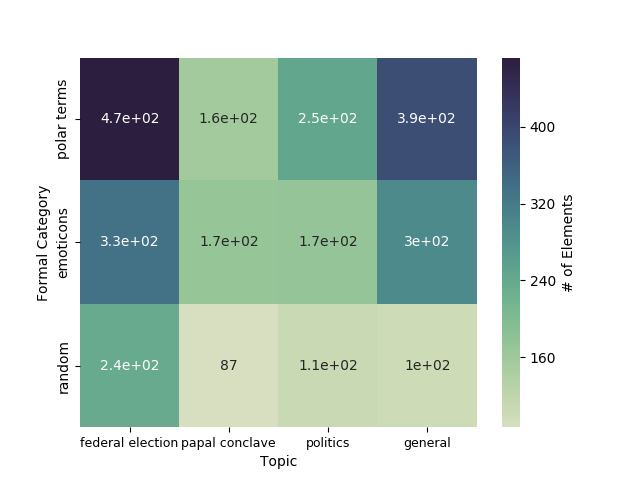
\includegraphics[width=\linewidth]{img/sentiment_stat.png}
  \caption{\texttt{Sentiments}}
\end{subfigure}%
\begin{subfigure}{.5\textwidth}
  \centering
  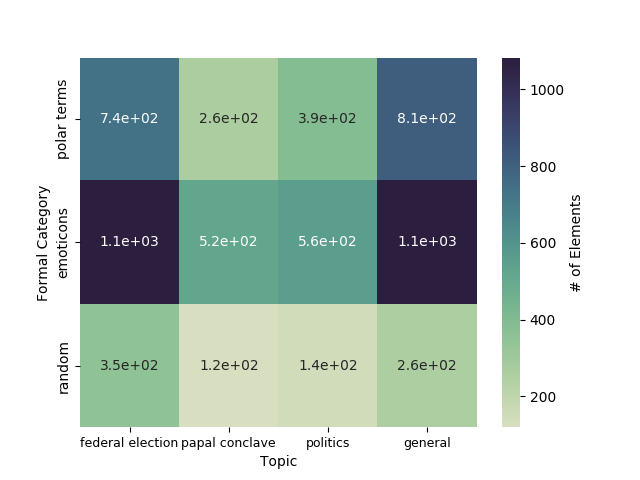
\includegraphics[width=\linewidth]{img/emo-expression_stat.png}
  \caption{\texttt{Emotional expressions}}
\end{subfigure}
}
\caption{Distribution of sentiments and emotional expressions across
  topics and formal categories.}\label{fig:distr}
\end{figure*}

\begin{figure*}[htbp!]
{
\centering
\begin{subfigure}{.5\textwidth}
  \centering
  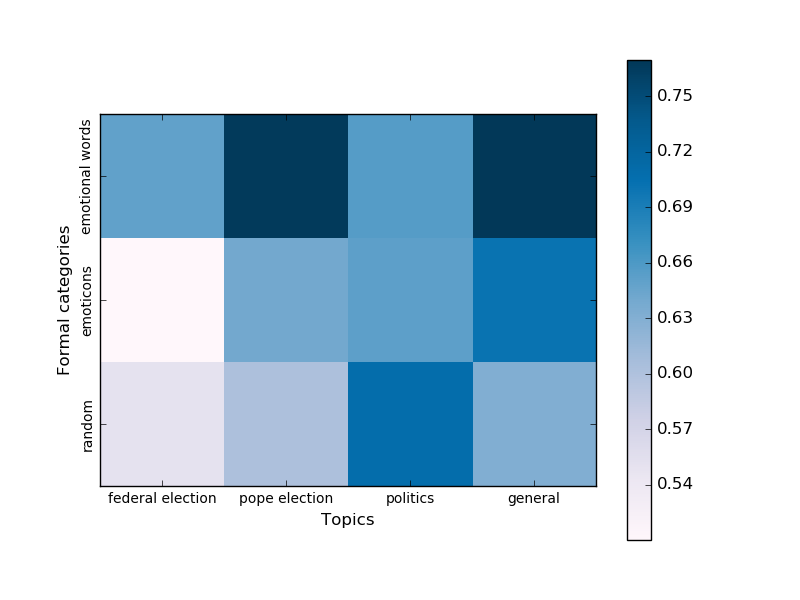
\includegraphics[width=\linewidth]{img/sentiment_agreement.png}
  \caption{\texttt{Sentiments}}
\end{subfigure}%
\begin{subfigure}{.5\textwidth}
  \centering
  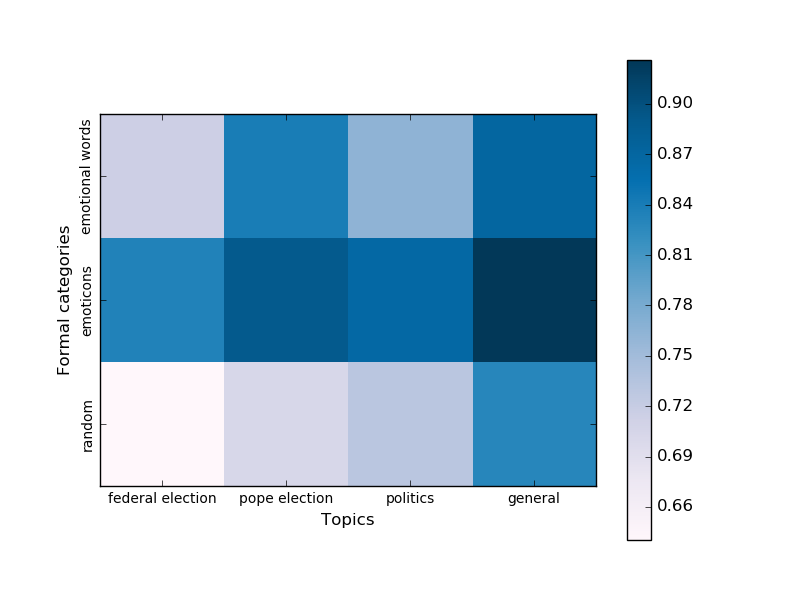
\includegraphics[width=\linewidth]{img/emo-expression_agreement.png}
  \caption{\texttt{Emotional expressions}}
\end{subfigure}
}
\caption{Inter-annotators agreement on sentiments and emotional
  expressions across topics and formal categories.}\label{fig:distr}
\end{figure*}

As can be seen from the scores, reaching a consensus about the
polarities of emotional terms was much easier than agreeing on the
value of this attribute for complete opinions.  Similar to
Example~\ref{example:sent-disagr}, one of the main reasons for these
disagreements were subjective opinions containing smileys, especially
in the cases when the polarity of the emoticon contradicted the
polarity of its preceding sentence, e.g., ``Ich hasse die
Piratenpartei \smiley{}'' (\emph{I hate the Pirate Party {\upshape
    \smiley{}}}).

Finally, to check how the selection criteria that we applied initially
for sampling our corpus affected the final distribution of sentiments
and polar expressions, we generated statistics plots on the
frequencies and agreement level of these elements in the annotated
dataset.  As can be seen from the figures, the stratification
according to topics and formal features has notably influenced both
the number of these elements and the difficulty of their
interpretation.

According to Figure \ref{fig:distr}, federal elections and topically
unfiltered tweets are the ones that contain the major part of the
opinions.  A similar tendency is also observed for emotional
expressions, though, in this case, the formal grouping appears to play
a more important role than topics.  Interestingly enough, the higher
number of polar terms does not necessarily imply a higher number of
targeted sentiments.  We can recognize that from the fact that, even
though most of the polar terms show up in the second row of the plot
(i.e., in microblogs with smileys), the biggest number of opinions
appear in row one (i.e., in tweets containing terms from the SentiWS
lexicon).

Regarding the inter-annotator agreement, we can see that the highest
reliability of annotated opinions is achieved on general tweets taken
from casual everyday conversations.  This group is also the one with
the highest IAA scores for emotional expressions.  A different
situation, however, is observed for these two element types as to the
formal groups of the tweets.  In this case, the first formal category
(i.e., tweets with lexicon terms) appears to comprise messages with
the most reliably annotated sentiments.  For emotional expressions,
however, the emoticons category, again, is the one with the highest
achieved result, whereas, for opinions, the agreement scores in this
row are among the lowest.  This finding suggests that, even though,
smileys are typically recognized as polar entities, the question
whether they relate to something particular in the tweet or rather
express the general mood of the author might often be difficult to
answer.

%% \subsection{Corpus Statistics}\label{subsec:snt:stat}

%% \begin{table}[h]
%%   \centering\small
%%   \caption[Sentiment corpus statistics]{Statistics on the annotated
%%     sentiment corpus.\\ POL = corpus part with discussions about
%%     general politic topics; FE = corpus part describing the federal
%%     election 2013; PE = corpus part with discussions about the Pope
%%     election 2013; GEN = part of the corpus containing tweets with no
%%     particular topic}
%%   \begin{tabular}{|>{\centering}p{0.15\textwidth}|*{4}{>{\centering}p{\oosixthClmnWidth}|}
%%       >{\centering\bfseries}p{\oosixthClmnWidth}|*{4}{>{\centering}p{\oosixthClmnWidth}|}
%%       >{\centering\bfseries}p{\oosixthClmnWidth}|}
%%     \hline

%%     \multirow{2}{*}{\parbox{0.13\textwidth}{\centering Markable Type}}
%%     & \multicolumn{5}{>{\centering}p{7\oosixthClmnWidth}|}{Annotator
%%       1} &
%%     \multicolumn{5}{>{\centering}p{7\oosixthClmnWidth}|}{Annotator
%%       2}\tabularnewline\cline{2-11}

%%     & POL & FE & PE & GEN & Total & POL & FE & PE & GEN &
%%     Total\tabularnewline\hline

%%     Sentiment & 212 & 222 & 163 & 131 & 728 & 317 & 335 & 314 & 305 & 1271
%%     \tabularnewline\hline

%%     Source & 101 & 119 & 68 & 73 & 361 & 114 & 109 & 94 & 85 & 402
%%     \tabularnewline\hline

%%     Target & 229 & 279 & 184 & 151 & 843 & 342 & 369 & 328 & 324 & 1363
%%     \tabularnewline\hline

%%     Emotional Expression & 727 & 689 & 581 & 811 & 2808 & 662 & 669 & 671 & 768 & 2770
%%     \tabularnewline\hline

%%     Intensifier & 16 & 32 & 14 & 44 & 106 & 31 & 35 & 31 & 58 & 155
%%     \tabularnewline\hline

%%     Diminisher & 2 & 4 & 3 & 2 & 11 & 2 & 9 & 4 & 2 & 17
%%     \tabularnewline\hline

%%     Negation & 18 & 15 & 23 & 14 & 70 & 33 & 33 & 31 & 23 & 120
%%     \tabularnewline\hline
%%   \end{tabular}
%%   \label{table:sentiment-agreement-topics}
%% \end{table}


\subsection{Related Work}
\newpage


% FILE: sentiment_lexica.tex  Version 0.01
% AUTHOR: Uladzimir Sidarenka

% This is a modified version of the file main.tex developed by the
% University Duisburg-Essen, Duisburg, AG Prof. Dr. Günter Törner
% Verena Gondek, Andy Braune, Henning Kerstan Fachbereich Mathematik
% Lotharstr. 65., 47057 Duisburg entstanden im Rahmen des
% DFG-Projektes DissOnlineTutor in Zusammenarbeit mit der
% Humboldt-Universitaet zu Berlin AG Elektronisches Publizieren Joanna
% Rycko und der DNB - Deutsche Nationalbibliothek

\chapter{Sentiment Lexicons}\label{sec:snt:lex}

The first avenue that we are going to explore using the obtained data
is an automatic prediction of polar terms.
% To this end, we will first present an updated version of our dataset
% in Subsection~\ref{subsec:snt-lex:data} in which our experts revised
% the annotations of words and idioms that were present in the existing
% German sentiment lexicons (GSL), but were not marked as emo-expressions
% in our data and, vice versa, were annotated as polar terms in the
% corpus, but absent in the analyzed polarity lists.
For this purpose, we are going to evaluate the existing German
sentiment lexicons on our corpus.  Since almost all of these resources
were created semi-automatically by first translating English polarity
lists and then manually post-editing the translated entries, we will
also look whether the original English sentiment lexicon generation
(SLG) methods would produce comparable results when applied to German
data directly.  Finally, we should analyze whether one of most popular
areas of research in contemporary computational
linguistics---distributed vector representations of words
\cite{Mikolov:13}---could be a more perspective way for deriving new
domain-specific sentiment lexicons in an unsupervised way.  In the
concluding step, we will investigate the effects of different
hyper-parameters and seed sets on these automatic approaches,
summarizing and concluding our findings in the last part of this
section.

\section{Data}\label{subsec:snt-lex:data}

In our experiments, we are going to use the complete data set labeled
by one of the experts as a test corpus in order to model a situation
where no annotated data are available during training (thus looking
for the most efficient unsupervised SLG technique) but make the
evaluation of tested methods as thorough as possible.  This set
comprises a total of 6,040 positive and 3,055 negative terms.
However, since many of these expressions represent emoticons, which,
on the one hand, are a priory absent in common lexical taxonomies such
as \textsc{WordNet} \cite{Miller:95,Miller:07} or \textsc{GermaNet}
\cite{Hamp:97} and therefore not amenable to SLG approaches relying on
these resources but, on the other hand, can be easily captured by
regular expressions, we decided to exclude non-alphabetic smileys
altogether from our study.  This left us with a set of 3,459 positive
and 2,755 negative labeled terms (1,738 and 1,943 unique expressions
respectively), whose $\kappa$-agreement run up to 0.59.  In addition
to that, we also selected a small subset of 400 tweets from the other
annotator as a development set for tuning hyper-parameters of
different approaches.

\section{Evaluation Metrics}\label{subsec:snt-lex:eval-metrics}

An important question which needs to be addressed before we procceed
with our experiments are the evaluation metrics that we should use to
measure the quality of (semi-)automatic sentiment lexicons.  Usually,
this quality is estimated either \textit{intrinsically} (i.e., taking
a lexicon in isolation and immediately assessing its accuracy) or
\textit{extrinsically} (i.e., considering the lexicon within the scope
of a bigger application such as a supervised classifier which utilizes
lexicon's entries as features).

Traditionally, intrinsic evaluation of English polarity lists amounts
to comparing these lists with the General Inquirer lexicon \cite[GI;
][]{Stone:66}---a manually compiled set of 11,895 words annotated with
their semantic categories---by taking the intersection of the two
resources and estimating the percentage of matches in which
automatically induced polar terms have the same polarity as the GI
entries.  This evaluation method, however, is somewhat problematic:
First of all, it is not easily transferable to other languages, since
even a manual translation of GI is not guaranteed to cover all
language- and domain-specific polar expressions.  Secondly, due to the
usage of intersection, this method does not penalize for a low recall
so that a lexicon consisting of just two terms \textit{good}$^+$ and
\textit{bad}$^-$ will have the highest possible score, often
surpassing polarity lists with a greater number of entries.  Finally,
such comparison does not account for polysemy.  As a result, an
ambiguous word only one of whose (possibly rare) senses is subjective
will always be ranked the same as a purely polar expression.

Unfortunately, an extrinsic evaluation does not always provide a
solution in this case, since, depending on the type of the extrinsic
system (e.g., a document classifier), it might still presuppose a
large data set for training other system components and, moreover,
might yield overly high scores, which, however, are mainly due to
these extrinsic components rather than the quality of the lexicon
itself.

Instead of using these approaches, we opt for a direct comparison of
the induced lexicons with an annotated corpus, since this type of
evaluation allows us to solve at least three of the previously
mentioned issues:
\begin{inparaenum}[(i)]
  \item It does account for the recall,
  \item it does accommodate polysemous words,\footnote{The annotators
      of the PotTS corpus were asked to annotate a polar expression
      iff its actual sense in the respective context was polar.} and
  \item it does preclude intermediate modules which might artificially
    boost the results.
\end{inparaenum}

In particular, in order to check a lexicon against the PotTS data set,
we construct a case-insensitive trie \cite[pp. 492--512]{Knuth:98}
from the lexicon entries and match this trie against the corpus text,
simultaneously comparing these entries with the actual word forms and
lemmas of corpus tokens.\footnote{We use the \texttt{TreeTagger}
  \cite{Schmid:95} to obtain lemma forms for corpus tokens.} A match
is considered correct iff the matched lexicon entry absolutely
corresponds to the (possibly lemmatized) expert's annotation and has
the same polarity as the one specified by the human coder.  That way,
we estimate the precision, recall, and \F{}-score for each particular
polarity class (positive, negative, and neutral), considering all
words absent in the lexicon as neutral.

\section{Semi-Automatic Lexicons}

We first use this metric to estimate the quality of the existing
German sentiment lexicons.  The most prominent of these resources are:
\begin{itemize}
\item the \textbf{German Polarity Clues} (GPC) by
  \citet{Waltinger:10}, which comprises 10,141 subjective entries
  automatically translated from the English sentiment lexicons
  Subjectivity Clues \cite{Wilson:05} and SentiSpin \cite{Takamura:05}
  with a subsequent manual correction of these translations and
  several synonyms and negated terms added by the authors;

\item the \textbf{SentiWS} (SWS) lexicon introduced by
  \citet{Remus:10}, which includes 1,818 positively and 1,650
  negatively connoted terms, also providing their part-of-speech tags
  and inflections (resulting in a total of 32,734 word forms).
  Similarly to the GPC, the authors used an English sentiment
  resource---the General Inquirer list by \citet{Stone:66}---to
  bootstrap the entries for their lexicon, manually revising these
  automatic translations afterwards.  In addition to that,
  \citet{Remus:10} also expanded their polarity set with words and
  phrases frequently co-occurring with positive and negative seed
  lexemes using collocation information obtained from a corpus of
  10,200 customer reviews or extracted from the German Collocation
  Dictionary \cite{Quasthoff:10};

\item and, finally, the \textbf{Zurich Polarity List} (ZPL) developed
  by \citet{Clematide:10}, which features 8,000 subjective entries
  taken from GermaNet synsets \cite{Hamp:97}.  These synsets were
  manually annotated with their prior polarities by human experts.
  Since the authors, however, found the number of polar adjectives
  obtained that way insufficient for running further classification
  experiments, they automatically enriched their lexicon with more
  attributive terms by analyzing conjoined collocations from a corpus
  using the method of \citet{Hatzivassi:97}.
\end{itemize}
% Since all of these lexicons were created semi-automatically by either
% automatically translating English polarity lists and then manually
% revising these translations (e.g., GPC and SWS) or by manually
% labeling an existing lexical resource and then automatically expanding
% this set (e.g., ZPL), their results should give us an upper bound on
% the fully automated approaches which we are going to test in the
% remaining parts of this section.

For our evaluation, we tested each of the three lexicons in
isolation\footnote{For the sake of these experiments, we excluded the
  auxiliary words ``aus'' (\emph{from}), ``der'' (\emph{the}),
  ``keine'' (\emph{no}), ``nicht'' (\emph{not}), ``sein'' (\emph{to
    be}), ``was'' (\emph{what}), and ``wer'' (\emph{who}) with their
  inflection forms from the German Polarity Clues lexicon, since these
  entries significantly worsened the evaluation results.} and also
evaluated their union and intersection, in order to check for
``synergy'' effects.  The results of these computations are shown in
Table~\ref{snt-lex:tbl:gsl-res}.

\begin{table}[h]
  \begin{center}
    \bgroup \setlength\tabcolsep{0.1\tabcolsep}\scriptsize
    \begin{tabular}{p{0.162\columnwidth} % first columm
        *{9}{>{\centering\arraybackslash}p{0.074\columnwidth}} % next nine columns
        *{2}{>{\centering\arraybackslash}p{0.068\columnwidth}}} % last two columns
      \toprule
      \multirow{2}*{\bfseries Lexicon} & %
      \multicolumn{3}{c}{\bfseries Positive Expressions} & %
      \multicolumn{3}{c}{\bfseries Negative Expressions} & %
      \multicolumn{3}{c}{\bfseries Neutral Terms} & %
      \multirow{2}{0.068\columnwidth}{\bfseries\centering Macro\newline \F{}} & %
      \multirow{2}{0.068\columnwidth}{\bfseries\centering Micro\newline \F{}}\\
      \cmidrule(lr){2-4}\cmidrule(lr){5-7}\cmidrule(lr){8-10}

      & Precision & Recall & \F{} & %
      Precision & Recall & \F{} & %
      Precision & Recall & \F{} & & \\\midrule
      %% \multicolumn{9}{|c|}{\cellcolor{cellcolor}Existing Lexicons}\\\hline

      % Class                     Precision              Recall                 F-score
      % positive                   0.209155             0.534630                 0.300680
      % negative                   0.194531             0.466468                 0.274561
      % neutral                    0.982806             0.923144                 0.952041
      % Macro-average              0.462164             0.641414                 0.509094
      % Micro-average              0.906173             0.906591                 0.906382

      GPC & 0.209 & 0.535 & 0.301 & %
      0.195 & 0.466 & 0.275 & %
      0.983 & 0.923 & 0.952 & %
      0.509 & 0.906 \\

      % Class                     Precision              Recall                 F-score
      % positive                   0.335225             0.435308                 0.378767
      % negative                   0.484006             0.343890                 0.402091
      % neutral                    0.976617             0.975014                 0.975815
      % Macro-average              0.598616             0.584737                 0.585557
      % Micro-average              0.952082             0.952045                 0.952064

      SWS & 0.335 & 0.435 & 0.379 & %
      0.484 & 0.344 & \textbf{0.402} & %
      0.977 & 0.975 & 0.976 & %
      0.586 & 0.952\\

      % Class                     Precision              Recall                 F-score
      % positive                   0.410806             0.423519                 0.417066
      % negative                   0.380378             0.352459                 0.365887
      % neutral                    0.976709             0.978684                 0.977696
      % Macro-average              0.589298             0.584887                 0.586883
      % Micro-average              0.954178             0.955459                 0.954818

      ZPL & 0.411 & 0.424 & 0.417 & %
      0.38 & 0.352 & 0.366 & %
      0.977 & 0.979 & 0.978 & %
      0.587 & 0.955 \\

      % Intersection
      % Class                     Precision              Recall                 F-score
      % positive                   0.527372             0.371942                 0.436225
      % negative                   0.617702             0.244411                 0.350240
      % neutral                    0.973299             0.990414                 0.981782
      % Macro-average              0.706124             0.535589                 0.589416
      % Micro-average              0.963883             0.963695                 0.963789

      GPC $\cap$ SWS $\cap$ ZPL & \textbf{0.527} & 0.372 & \textbf{0.436} & %
      \textbf{0.618} & 0.244 & 0.35 & %
      0.973 & \textbf{0.99} & \textbf{0.982} & %
      \textbf{0.589} & \textbf{0.964} \\

      % Union
      % Class                     Precision              Recall                 F-score
      % positive                   0.201544             0.561745                 0.296654
      % negative                   0.195185             0.531669                 0.285543
      % neutral                    0.984751             0.916952                 0.949643
      % Macro-average              0.460493             0.670122                 0.510613
      % Micro-average              0.899292             0.902381                 0.900834

      GPC $\cup$ SWS $\cup$ ZPL & 0.202 & \textbf{0.562} & 0.297 & %
      0.195 & \textbf{0.532} & 0.286 & %
      \textbf{0.985} & 0.917 & 0.95 & %
      0.51 & 0.901 \\\bottomrule
    \end{tabular}
    \egroup
    \caption{Evaluation of semi-automatic German sentiment lexicons.\\
      {\small GPC -- German Polarity Clues \cite{Waltinger:10}, SWS --
        SentiWS \cite{Remus:10}, ZPL -- Zurich Polarity Lexicon
        \cite{Clematide:10}}}
    \label{snt-lex:tbl:gsl-res}
  \end{center}
\end{table}

As can be seen from the table, the intersection of all three polarity
lists achieves the best results on both positive and neutral classes,
also yielding the best scores in terms of the macro- and
micro-averaged $F$-measures.  One of the main reasons for this success
is a relatively high precision of this list for all but the neutral
polarity class, where it is outperformed by the union of all three
resources.  Not surpisingly, the union also shows the highest recall
of positive and negative terms among all compared polarity lists.
Regarding the figures attained by the individual lexicons, the best
results here are achieved by the SentiWS resource~\cite{Remus:10},
which shows the highest \F{}-score for negative terms, and the Zurich
Polarity List~\cite{Clematide:10}, which achieves the second best
macro-averaged \F{}-result, coming very close to the scores attained
by the intersection of the three resources.

\section{Automatic Methods}

A natural question which arises upon the evaluation of the existing
semi-automatic lexicons is how well fully automatic methods can
perform in comparison with these lists.  According to
\citet[p. 79]{Liu:12}, most of automatic SLG algorithms can be grouped
into dictionary- and corpus-based ones.  The former systems induce
polarity lists from monolingual thesauri or lexical databases such as
the Macquarie Dictionary \cite{Bernard:86} or \textsc{WordNet}
\cite{Miller:95}.  A clear advantage of these methods is their
relatively high precision as they operate on carefully verified data
enriched with hand-crafted meta information.  At the same time, this
precision might come at the cost of a reduced recall especially for
the domains where the language changes occur very rapidly, and new
terms are being coined in a flash.  In contrast to this, corpus-based
systems can operate directly on unannotated in-domain data, having a
direct access to all neologisms, but they often have to deal with an
extreme noisiness of their input and consequently suffer from a lower
accuracy.  Since it was unclear which of these strengths and
weaknesses would have a stronger influence on the net results, we
decided to reimplement the most commonly used algorithms from both of
these paradigms and evaluate them on our corpus.

\subsection{Dictionary-Based Methods}

The presumably first SLG system which inferred a set of polar terms
form a manually created lexical database was proposed by
\citet{Hu:04}.  In their work on sentiment classification and
summarization of cutomer reviews, the authors determined semantic
orientation of adjectives (which were supposed to be the most relevant
part of speech for mining people's opinions) by taking a list of seed
terms with known semantic orientation and propagating the polarity
values of these words to their synonyms found in \textsc{WordNet}
\cite{Miller:95}.  A similar procedure was applied to the antonymous
relations with the polarity scores being reversed during the
propagation.  The expansion continued until no more adjective could be
reached via the synonymy-antonymy links.
% Unfortunately, no intrinsic evaluation of the resulting lexicon was
% performed in this work---the authors only report their results on
% recognizing subjective sentences and classifying their polarity, where
% they attain average \F-scores of 0.667 and 0.842 respectively.

Later on, this approach was refined by \citet{Blair-Goldensohn:08},
who obtained polarity labels for new words by multiplying a vector
$\vec{v}$ containing polarity scores of known seed terms (-1 for
negative expressions and 1 for positive terms) with an adjacency
matrix $A$ constructed from \textsc{WordNet} synsets.  The value of
the adjacency cell $a_{ij}$ in this matrix was set to $\lambda=0.2$ if
there was a synonymy link between the synsets $i$ and $j$ and to
$-\lambda$ if these synsets were antonymous to each other.  By
performing this multiplication multiple times and setting the vector
$\vec{v}$ to the result of the previous iteration, the authors ensured
that the polarity scores were propagated transitively through the
network, decaying by a constant factor ($\lambda$) with the increasing
path length from the original
seeds.% This method again was evaluated only extrinsically---the
% authors tested their complete sentiment summarization system, which
% used the sentiment scores for individual words as features for a
% maximum-entropy classifier.

With various modifications, the core idea of propagating the polarity
classes through a lexical graph was adopted in almost all of the
following dictionary-based works: \citet{Kim:04,Kim:06}, for instance,
used a similar method to determine the polarity of adjectives and
verbs given a small set of seed terms with known orientation.  In
particular, the likelihood of a new word $w$ belonging to the class $c
\in \{\textrm{positive, negative, neutral}\}$ was computed as:
\begin{equation*}
  P(c|w) = \argmax_{c}P(c)P(w|c) = \argmax_{c}P(c)\frac{\sum\limits_{i=1}^{n}count(syn_i, c)}{count(c)},
\end{equation*}
where $P(c)$ was the prior probability of the polar class (estimated
as the number of words with the given orientation $c$ divided by the
total number of terms considered), $count(syn_i, c)$ meant the number
of times a seed term from class $c$ appeared in a synset of $w$, and
$count(c)$ denoted the total number of synsets containing a seed item.
Starting from a seed set of 34 adjectives and 44 verbs, the authors
successively expanded their lexicon to a list of 18,192 terms. %  and
% evaluated it on a manually labeled collection of 462 adjectives and
% 502 verbs taken from the TOEFL test and analyzed by two human experts.
% The reported average accuracy for this method run up to 68.48\% for
% adjectives and 74.28\% for verbs with their recall being equal to
% 93.07\% and 83.27\% respectively.  It should, however, be noted that
% \citet{Kim:04} used a lenient metric for their computation by
% considering neutral and positive terms as the same class which could
% significantly boost the results.

% An alternative way of bootstrapping polarities for adjectives was
% proposed by \citet{Kamps:04}.  The authors estimated the orientation
% of the given term by computing the difference between the shortest
% path lengths of this word to the prototypic positive and negative
% lexemes---``good'' and ``bad''.  For example, the polarity score of
% the adjective ``honest'' was calculated as
% \begin{equation*}
%   POL(honest) = \frac{d(\textrm{honest}, \textrm{bad}) - d(\textrm{honest}, \textrm{good})}%
%   {d(\textrm{bad}, \textrm{good})} = \frac{6 - 2}{4} = 1,
% \end{equation*}
% where $d(w_1, w_2)$ means the geodesic (shortest-path) distance
% between the words $w_1$ and $w_2$ in the \textsc{WordNet} graph.  The
% respective orientation of this term was then correspondingly set to
% \texttt{positive} according to the sign of the obtained
% $POL$-value. \citet{Kamps:04} evaluated the accuracy of their method
% on the General Inquirer lexicon \cite{Stone:66} by comparing the terms
% with non-zero scores to the entries from this resource, getting
% 68.19\% of correct predictions on a set of 349 adjectives.

One of the most popular dictionary-based approaches to date, however,
was proposed by \citet{Esuli:06c}.  Starting with the positive and
negative seed sets of \citet{Turney:03} and considering the rest of
the terms as objective if these words neither appeared in the
aforemention seed lists nor had a subjective tag in the General
Inquirer lexicon \cite{Stone:66}, the authors successively expanded
these sets for $k \in \{0, 2, 4, 6\}$ iterations by following the
synonymy-antonymy links similarly to the method of \citet{Hu:04}.  In
addition to that, in each of these steps, they trained two types of
ternary classifiers---Rocchio and SVM---using tfidf-vectors of the
training glosses (whose amount was different in each iteration) as
input features.  In the concluding step, \citet{Esuli:06c} united
these classifiers into one ensemble and assigned normalized class
scores returned by this committee to the remaining \textsc{WordNet}
synsets.\footnote{In contrast to other works, the method of
  \citet{Esuli:06c} returns a 3-tuple of scores for each polarity
  class (positive, negative, and neutral) without attempting to
  classify them into these categories.}
% This time, the evaluation was run on both the intersection with the
% GI~lexicon~\cite{Stone:66} and a manually annotated subset of
% \textsc{WordNet} synsets, yielding 66\% accuracy for the former
% metric.\footnote{Note that different publications on
% \textsc{SentiWordNet} report different configuration settings,
% cf. \citet{Esuli:05}, \citet{Esuli:06a}, \citet{Esuli:06b}, and
% \citet{Esuli:06c}.  In our experiments, we will rely on the setup
% described in last paper as the most recent description of this
% approach.}

Another graph-based approach was proposed by \citet{Rao:09}.  In their
work, the authors experimented with three different methods of
assigning polarity scores to synsets:
\begin{inparaenum}[\itshape a\upshape)]
\item deterministic min-cut \cite{Blum:01},
\item randomized min-cut \cite{Blum:04}, and
\item the label propagation algorithm by \citet{Zhu:02}.
\end{inparaenum}
% An evaluation of these systems on the GI lexicon \cite{Stone:66}
% showed significant improvement over the previous baselines of
% \citet{Kamps:04} and \citet{Kim:06}.

Other notable works on dictionary-based lexicon generation include
those by \citet{Mohammad:09}, who generated their seed set using
antonymous morphological patterns (e.g.,
\emph{logical}---\emph{illogical}, \emph{honest}---\emph{dishonest},
\emph{happy}---\emph{unhappy}) and subsequently expanded these seed
sets with the help of the Macquarie Thesaurus \cite{Bernard:86};
\citet{Awadallah:10}, who adopted a random walk approach, estimating
the polarity of an unknown word by taking the difference between an
average number of steps a random walker had to make in order to reach
a term from positive or negative set; and \citet{Dragut:10}, who
deduced the polarities of new words using manually specified inference
rules.

% Since almost all of the presented approaches used \textsc{WordNet}---a
% large lexical database with more than 117,000 synsets---and evaluated
% their results in vitro (using the General Inquirer lexicon
% \cite{Stone:66}), it remains unclear how these methods would work for
% languages with smaller lexical resources and whether they would
% perform equally well in vivo (when tested on a real-life corpus).
% Moreover, because General Inquirer is a generic standard-language
% dictionary, it is also not obvious whether the systems that perform
% best on this list would be also applicable to more colloquial domains.

For our experiments, we reimplemented the approaches by \citet{Hu:04},
\citet{Blair-Goldensohn:08}, \citet{Kim:04,Kim:06}, \citet{Esuli:06c},
\citet{Rao:09}, and \citet{Awadallah:10}, applying these methods to
\textsc{GermaNet}---the German equivalent of the English
\textsc{WordNet} \cite{Hamp:97}\footnote{Throughout our experiments,
  we will use \textsc{WordNet} Version 3.0 and \textsc{GermaNet}
  Version 9.}---and subsequently evaluating their results on our
Twitter corpus.

In order to make this comparison more fair, we used the same set of
the initial seed terms for all tested methods.  For this purpose, we
translated the original list of 14 subjectively connoted English
adjectives suggested by \citet{Turney:03}---\emph{good}$^+$,
\emph{nice}$^+$, \emph{excellent}$^+$, \emph{positive}$^+$,
\emph{fortunate}$^+$, \emph{correct}$^+$, \emph{superior}$^+$,
\emph{bad}$^-$, \emph{nasty}$^-$, \emph{poor}$^-$,
\emph{negative}$^-$, \emph{unfortunate}$^-$, \emph{wrong}$^-$, and
\emph{inferior}$^-$---into German, getting a total of 20 seeds (10
positive and 10 negative adjectives) due to multiple possible
translations of the same words.\footnote{The reimplemented methods and
  translated seed sets used in these experiments are available online
  at \url{https://github.com/WladimirSidorenko/SentiLex}.}
Furthermore, to settle the differences between the binary and ternary
approaches (i.e., those methods that only differentiated between the
positive and negative classes and those ones which also distinguished
neutral terms as a separate category), we additionally enriched the
translated seed set with 10 purely objective
adjectives---\emph{neutral}$^0$, \emph{objective}$^0$,
\emph{technical}$^0$, \emph{chemical}$^0$, \emph{physical}$^0$,
\emph{material}$^0$, \emph{bodily}$^0$, \emph{financial}$^0$,
\emph{theoretical}$^0$, and \emph{practical}$^0$---letting all
evaluated classifiers work in the ternary mode.  Finally, since
different methods relied on various notions of synonymous relations
(e.g., \citet{Hu:04} only considered two words as synonyms if they
appeared together in the same synset, whereas \citet{Esuli:06c},
\citet{Rao:09}, and \citet{Awadallah:10} also considered
hyper-hyponymous connections as valid edges for propagating the
polarity of the seed terms), we decided to unify this aspect too,
letting all systems work with an extended set of links.  In so doing,
we not only established an edge between any two terms appearing in the
same synset but also drew a tie between all words whose synsets were
conected via the inter-synset links \texttt{has\_participle},
\texttt{has\_pertainym}, \texttt{has\_hyponym}, \texttt{entails}, or
\texttt{is\_entailed\_by}.\footnote{For the method of
  \citet{Esuli:06c}, we only used the inter-synset links, dispensing
  with the intra-synset connections, as those were the only relations
  utilized in their original work.} We intentionally skipped the
relations \texttt{has\_hypernym} and \texttt{is\_related\_to} when
constructing the graph, since hypernyms were not guaranteed to
preserve the polarity of their children---e.g.,
``bewertungsspezifisch'' (\emph{appraisal-specific}) is a neutral term
in contrast to its immediate hyponyms ``gut'' (\emph{good}) and
``schlecht'' (\emph{bad})---and the relatedness links
(\texttt{is\_related\_to}) could connect both synonyms and antonyms of
the same term---e.g., this relation type simultaneoulsy holds between
the words ``Form'' (\emph{shape}) and ``unf\"ormig''
(\emph{misshapen}) and ``Dame'' (\emph{lady}) and ``damenhaft''
(\emph{ladylike}).

We fine-tuned the hyper-parameters of the evaluated approaches using
grid search and optimizing the macro-averaged \F{}-score on the
development set.  In particular, instead of waiting for the full
convergence of the eigenvector in the approach of
\citet{Blair-Goldensohn:08}, we set the maximum number of times the
polarity vector was multiplied with the adjacency matrix to five.  Our
experiments showed that this limitation had a crucial impact on the
quality of the resulting polarity list (e.g., after five
multiplications, the average precision of the recognized positive
terms amounted to 0.499, reaching an average \F{}-score of 0.26 for
this class; after ten more iterations, however, this precision
decreased dramatically to 0.043, pulling the class-specific \F{}-score
down to 0.078).  In the same vein, we limited the maximum number of
iterations in the label-propagation method of \citet{Rao:09} to 300,
although the effect of this setting was much weaker than in the
previous case (by comparison, the scores obtained after 30 runs
differed only by a few hundredths from the results observed after 300
iterations).  Finally, in the method of \citet{Awadallah:10}, we
allowed for seven simultaneous walkers with a maximum of 17 steps
each, considering a term as polar if more than a half of these walkers
agreed on the polarity of the analyzed term.

\begin{table}[h]
  \begin{center}
    \bgroup \setlength\tabcolsep{0.1\tabcolsep}\scriptsize
    \begin{tabular}{p{0.142\columnwidth} % first columm
        >{\centering\arraybackslash}p{0.06\columnwidth} % second columm
        *{9}{>{\centering\arraybackslash}p{0.072\columnwidth}} % next nine columns
        *{2}{>{\centering\arraybackslash}p{0.058\columnwidth}}} % last two columns
      \toprule
      \multirow{2}*{\bfseries Lexicon} & %
      \multirow{2}{0.06\columnwidth}{\bfseries\centering \# of\newline{} Terms} & %
      \multicolumn{3}{c}{\bfseries Positive Expressions} & %
      \multicolumn{3}{c}{\bfseries Negative Expressions} & %
      \multicolumn{3}{c}{\bfseries Neutral Terms} & %
      \multirow{2}{0.068\columnwidth}{\bfseries\centering Macro\newline \F{}} & %
      \multirow{2}{0.068\columnwidth}{\bfseries\centering Micro\newline \F{}}\\
      \cmidrule(lr){3-5}\cmidrule(lr){6-8}\cmidrule(lr){9-11}

      & & Precision & Recall & \F{} & %
      Precision & Recall & \F{} & %
      Precision & Recall & \F{} & & \\\midrule
      %% \multicolumn{9}{|c|}{\cellcolor{cellcolor}Existing Lexicons}\\\hline

      % Class                     Precision              Recall                 F-score
      % positive                   0.770601             0.101975                 0.180115
      % negative                   0.567901             0.017139                 0.033273
      % neutral                    0.963176             0.999227                 0.980870
      % Macro-average              0.767226             0.372780                 0.398086
      % Micro-average              0.962404             0.962216                 0.962310

      \textsc{Seed Set} & 20 & \textbf{0.771} & 0.102 & 0.18 & %
      0.568 & 0.017 & 0.033 & %
      0.963 & \textbf{0.999} & \textbf{0.981} & %
      0.398 & \textbf{0.962}\\

      % Class                     Precision              Recall                 F-score
      % positive                   0.160648             0.266136                 0.200355
      % negative                   0.199554             0.133383                 0.159893
      % neutral                    0.969132             0.960190                 0.964640
      % Macro-average              0.443111             0.453236                 0.441629
      % Micro-average              0.930521             0.930387                 0.930454

      HL & 5,745 & 0.161 & 0.266 & 0.2 & %
      0.2 & 0.133 & 0.16 & %
      0.969 & 0.96 & 0.965 & %
      0.442 & 0.93\\

      % Class                     Precision              Recall                 F-score
      % positive                   0.502551             0.232243                 0.317678
      % negative                   0.284571             0.092772                 0.139927
      % neutral                    0.967533             0.991262                 0.979254
      % Macro-average              0.584885             0.438759                 0.478953
      % Micro-average              0.958888             0.958769                 0.958828

      BG & 1,895 & 0.503 & 0.232 & \textbf{0.318} & %
      0.285 & 0.093 & 0.14 & %
      0.968 & 0.991 & 0.979 & %
      \textbf{0.479} & 0.959\\

      % Class                     Precision              Recall                 F-score
      % positive                   0.715608             0.159446                 0.260786
      % negative                   0.269406             0.043964                 0.075593
      % neutral                    0.964973             0.996744                 0.980601
      % Macro-average              0.649996             0.400051                 0.438993
      % Micro-average              0.961759             0.961571                 0.961665

      KH & 356 & 0.716 & 0.159 & 0.261 & %
      0.269 & 0.044 & 0.076 & %
      0.965 & 0.997 & \textbf{0.981} & %
      0.439 & \textbf{0.962}\\

      % Class                     Precision              Recall                 F-score
      % positive                   0.041632             0.564397                 0.077544
      % negative                   0.033042             0.255216                 0.058510
      % neutral                    0.981022             0.689113                 0.809557
      % Macro-average              0.351899             0.502909                 0.315204
      % Micro-average              0.612283             0.678788                 0.643823

      ES & 39,181 & 0.042 & \textbf{0.564} & 0.078 & %
      0.033 & \textbf{0.255} & 0.059 & %
      \textbf{0.981} & 0.689 & 0.81 & %
      0.315 & 0.644\\

      % Class                     Precision              Recall                 F-score
      % positive                   0.070618             0.422045                 0.120992
      % negative                   0.215708             0.072653                 0.108696
      % neutral                    0.972028             0.873448                 0.920105
      % Macro-average              0.419451             0.456049                 0.383264
      % Micro-average              0.848630             0.849470                 0.849050

      RR$_{\textrm{mincut}}$ & 8,060 & 0.07 & 0.422 & 0.12 & %
      0.216 & 0.073 & 0.109 & %
      0.972 & 0.873 & 0.92 & %
      0.383 & 0.849\\

      % Class                     Precision              Recall                 F-score
      % positive                   0.566825             0.176245                 0.268885
      % negative                   0.571429             0.046200                 0.085488
      % neutral                    0.965423             0.996716                 0.980820
      % Macro-average              0.701225             0.406387                 0.445064
      % Micro-average              0.962125             0.961956                 0.962040

      RR$_{\textrm{lbl-prop}}$ & 1,105 & 0.567 & 0.176 & 0.269 & %
      \textbf{0.571} & 0.046 & 0.085 & %
      0.965 & 0.997 & \textbf{0.981} & %
      0.445 & \textbf{0.962}\\

      % Class                     Precision              Recall                 F-score
      % positive                   0.768182             0.099617                 0.176363
      % negative                   0.567901             0.017139                 0.033273
      % neutral                    0.963126             0.999233                 0.980847
      % Macro-average              0.766403             0.371996                 0.396828
      % Micro-average              0.962358             0.962170                 0.962264

      AR & 23 & 0.768 & 0.1 & 0.176 & %
      0.568 & 0.017 & 0.033 & %
      0.963 & \textbf{0.999} & \textbf{0.981} & %
      0.397 & \textbf{0.962}\\

      % Class                     Precision              Recall                 F-score
      % positive                   0.600858             0.165046                 0.258960
      % negative                   0.567442             0.045455                 0.084167
      % neutral                    0.965096             0.997212                 0.980891
      % Macro-average              0.711132             0.402571                 0.441339
      % Micro-average              0.962327             0.962170                 0.962249

      HL $\cap$ BG $\cap$ RR$_{\textrm{lbl}}$ & 752 & 0.601 & 0.165 & 0.259 & %
      0.567 & 0.045 & 0.084 & %
      0.965 & 0.997 & \textbf{0.981} & %
      0.441 & \textbf{0.962}\\

      % Class                     Precision              Recall                 F-score
      % positive                   0.165676             0.287651                 0.210254
      % negative                   0.191198             0.145678                 0.165363
      % neutral                    0.969910             0.957599                 0.963716
      % Macro-average              0.442262             0.463643                 0.446444
      % Micro-average              0.928663             0.928590                 0.928626

      HL $\cup$ BG $\cup$ RR$_{\textrm{lbl}}$ & 6,258 & 0.166 & 0.288 & 0.21 & %
      0.191 & 0.146 & \textbf{0.165} & %
      0.97 & 0.958 & 0.964 & %
      0.446 & 0.929\\\bottomrule
    \end{tabular}
    \egroup
    \caption{Evaluation of dictionary-based approaches.\\ {\small HL
        -- \citet{Hu:04}, BG -- \citet{Blair-Goldensohn:08}, KH --
        \citet{Kim:04}, ES -- \citet{Esuli:06c}, RR -- \citet{Rao:09},
        AR -- \citet{Awadallah:10}}}
    \label{snt-lex:tbl:lex-res}
  \end{center}
\end{table}

The results of our reimplementations are shown in
Table~\ref{snt-lex:tbl:lex-res}.  As can be seen from the table, the
results of the automatic methods are significantly lower than the
figures obtained by the semi-automatic lexicons.  The best
macro-averaged \F{}-score for all three classes (0.479) is attained by
the method of \citet{Blair-Goldensohn:08}, which is still 0.11 points
worse than the peak result achieved by the intersection of the GPC,
SentiWS, and Zurich Polarity lists (0.589).  Apart from this, the
situation for the dictionary-based methods in general is much more
varied than in the case of the existing German lexicons as different
systems can achieve best scores on just some aspects of certain
classes but can hardly attain best overall results in all categories.
This is, for instance, the case for the positive and negative
polarities, where the best precision is reached by the seed set in the
first case and the label propagation algorithm by \citet{Rao:09} in
the second case.  However, with respect to the recall, both of these
polarity lists perform notably worse than the approach by
\citet{Esuli:06c}.  Yet other systems---the matrix-vector method by
\citet{Blair-Goldensohn:08} and the union of the three overall
top-scoring systems respectively---reach the highest \F{}-scores for
these two classes.  Nevertheless, we can still notice three main
tendencies in this evaluation:
\begin{inparaenum}[\itshape a\upshape)]
\item the method by \citet{Esuli:06c} generally gets the highest
  recall of polar terms and, consequently, achieves the best precision
  in recognizing neutral words, but suffers from a low precision for
  the positive and negative polarities,
\item simultaneously five systems attain the same best \F{}-scores on
  recognizing neutral terms, which, in turn, leads to the best
  micro-averaged \F{}-results for all polarity classes, and, finally,
\item the system of \citet{Blair-Goldensohn:08} achieves its high
  macro-averaged performance mainly due to a relatively good balance
  of precision and recall for the main polarity groups, but fails to
  attain best results on any one of these single aspects.
\end{inparaenum}

% Seed Sets:

% Hu-Liu were using 30 adjectives, but they only provided some
% examples: great, fantastic, nice, cool, bad, and dull

% Blair-Goldensohn: do not report (In our experiments, the original
% seed set contained 20 negative and 47 positive words that were
% selected by hand to maximize domain coverage, as well as 293 neutral
% words that largely consist of stop words.)

% Kim-Hovy (2004): To start the seed lists we selected verbs (23
% positive and 21 negative) and adjectives (15 positive and 19
% negative), adding nouns later.  But they, again, do not report
% specific examples.

% Kim-Hovy (2006): We described a word classification system to de-
% tect opinion-bearing words in Section 2.1. To ex- amine its
% effectiveness, we annotated 2011 verbs and 1860 adjectives, which
% served as a gold stan- dard 7 . These words were randomly selected
% from a collection of 8011 English verbs and 19748 English
% adjectives. We use training data as seed words for the WordNet
% expansion part of our algorithm.

% Esuli/Sebastiani: Lp and Ln are two small sets, which we have
% defined by manually selecting the intended synsets4 for 14
% "paradigmatic" Positive and Negative terms (e.g., the Positive term
% nice, the Negative term nasty) which were used as seed terms in
% (Turney and Littman, 2003).  The Lo set is treated differently from
% Lp and Ln, because of the inherently "complementary" nature of the
% Objective category (an Objective term can be defined as a term that
% does not have either Positive or Negative characteristics). We have
% heuristically defined Lo as the set of synsets that (a) do not
% belong to either T rK p or T rK n , and (b) contain terms not marked
% as either Positive or Negative in the General Inquirer lexicon
% (Stone et al., 1966); this lexicon was chosen since it is, to our
% knowledge, the largest manually annotated lexicon in which terms are
% tagged according to the Positive or Negative categories.

% Rao-Ravichandran: All experiments reported in Sections 4.1 to 4.5
% use the data described above with a 50-50 split so that the first half
% is used as seeds and the sec- ond half is used for test.

% Awdallah: After (Turney, 2002), we use our method to predict
% semantic orientation of words in the General Inquirer lexicon (Stone
% et al., 1966) using only 14 seed words.

% seed sets: (Turney and Littman, 2003); SentiWS (Remus, 2010)

\subsection{Corpus-Based Methods}

An alternative way to generate polarity lists is to use corpus-based
approaches.  In contrast to dictionary-based methods, these systems
typically operate immediately on raw texts of the target domain and
are, therefore, virtually independent of any manually annotated
linguistic resources.  This flexibility, however, might come at the
cost of a reduced accuracy due to an inherent noisiness of the
unlabeled data.

A pioneering work on these algorithms was done by
\citet{Hatzivassi:97}.  Based on the assumption that coordinately
conjoined adjectives typically share the same semantic orientation,
the authors trained a supervised logisitic classifier which predicted
the degree of dissimilarity between two co-occurring adjectival terms.
In the next step, they constructed a word graph, drawing a link
between any two adjectives which appeared in the same coordinative
pair and considering the predicted dissimilarity scores between these
words as their respective edge weights.  In the final stage, the
authors partitioned this graph into two parts and ascribed the
positive polarity to the bigger cluster.
% This method achieved an overall accuracy of 82.05\%
% on predicting the polarity of a subset of manually annotated
% adjectives when trained on the rest of these hand-labeled data.

Later on, this approach was further refined by \citet{Takamura:05},
who tried to unite dictionary- and corpus-based methods into a single
probabilistic framework.  To this end, the authors adopted the Ising
spin model from the statistical mechanics, considering terms found in
\textsc{WordNet} \cite{Miller:95}, the Wall Street Journal and Brown
corpora as electrons in a unified ferromagnetic lattice.  They
established a link between any two electrons whose corresponding terms
appeared in synonymous synsets or coordinately conjoined pairs in any
of the two corpora.  Taking into account the a priori known polarities
of the seed terms, they then approximated the most likely polarity
combination in this graph over all possible polarity assignments.
% reaching 91.5\% accuracy at predicting polarity of the manually
% labeled subjective terms from the General Inquirer lexicon
% \cite{Stone:66}.

Another way to induce a sentiment lexicon from a corpus was proposed
by \citet{Turney:03}, who derived a set of polarity terms by computing
the ratio of PMI-associations between potential words and a predefined
set of positive and negative seeds.  In particular, the semantic
orientation score of the given word $w$ was defined as:
\begin{equation*}
  \textrm{SO-A}(w) = \sum_{w_p\in\mathcal{P}}PMI(w, w_p) - \sum_{w_n\in\mathcal{N}}PMI(w, w_n),
\end{equation*}
where $\mathcal{P}$ was the set of positive seed terms, $\mathcal{N}$
denoted the collection of negative words, and the $PMI$ score was
normally computed as the log-ratio $PMI(w, w_x) = \log_2\frac{p(w,
  w_x)}{p(w)p(w_x)}$.  The joint probability $p(w, w_x)$ in the last
equation was calculated with the help of the
AltaVista\footnote{\url{www.altavista.com}} NEAR operator as the
number of hits returned by the ``$w\textrm{ NEAR }w_x$'' query divided
by the total number of documents indexed by this search engine.

This method was also successfully adapted to Twitter by
\citet{Kiritchenko:14}.  Using the distantly supervised corpus of
\citet{Go:09} and a separate collection of 775,000 tweets gathered
solely for the purpose of their experiments, the authors created two
sentiment lexicons---the Sentiment140 and Hashtag Sentiment Base
Lexicon---using the semantic orientation formula described above.
However, instead of querying AltaVista for computing the joint
probability scores, the authors estimated these values as the number
of times a potential candidate appeared in distantly labeled positive
(negative) tweets divided by the total number of tweets in their
collection.  In a similar vein, \citet{Severyn:15a} compiled their
list of polar terms by training an SVM classifier on the distantly
labeled corpus of \citet{Go:09} and using lexical n-grams extracted
from these tweets as features.  In the final step, the authors
included tokens with the highest learned weights into their final
polarity list.

Graphical methods for corpus-based lexicon induction were advocated by
\citet{Velikovich:10} and \citet{Feng:11}.  The former work proposed
an adaptation of the label-propagation algorithm previously suggested
by \citet{Rao:09} with the core difference that, instead of taking a
weighted average of all incident scores for a potential subjective
term, the authors took the maximum value propagated from a seed in
order to prune unreliable, noisy corpus connections.  The latter work
derived a list of subjectively connoted events and their associated
verb predicates using two popular approaches from information
retrieval---the PageRank \cite{Brin:98} and HITS algorithms
\cite{Kleinberg:99}.

For our experiments, we reimplemented the approaches by
\citet{Takamura:05}, \citet{Velikovich:10}, \citet{Kiritchenko:14} and
\citet{Severyn:15}, and applied these methods to the German Twitter
Snapshot \cite{Scheffler:14}---a collection of 24~M German microblogs
which we previously used to sample the data for our sentiment corpus.
We constructed the collocation graph from the lemmatized word forms of
this snapshot, skipping all words which appeared less than four times
in the analyzed data.  We again were using the \texttt{TreeTagger}
\cite{Schmid:95} for lemmatization and \texttt{GermaNet} for deriving
auxiliary semantic links between words for the method of
\citet{Takamura:05}.  Similarly to the previous experiments, we
fine-tuned all hyper-parameters (including the number of the induced
polar terms) by maximizing the macro-averaged \F{}-score on the
development set.  In particular, we set the $\beta$ constant in the
method by \citet{Takamura:05} to 0.8 and the maximum number of
iterations in the method by \citet{Velikovich:10} to 20.

% \cite{Lau:11} \citet{Bross:13} \citet{Tai:13} \citet{Yang:14}
% \citet{Bravo-Marquez:15}

% \begin{figure}[hbtp!]
% {
%   \centering
%   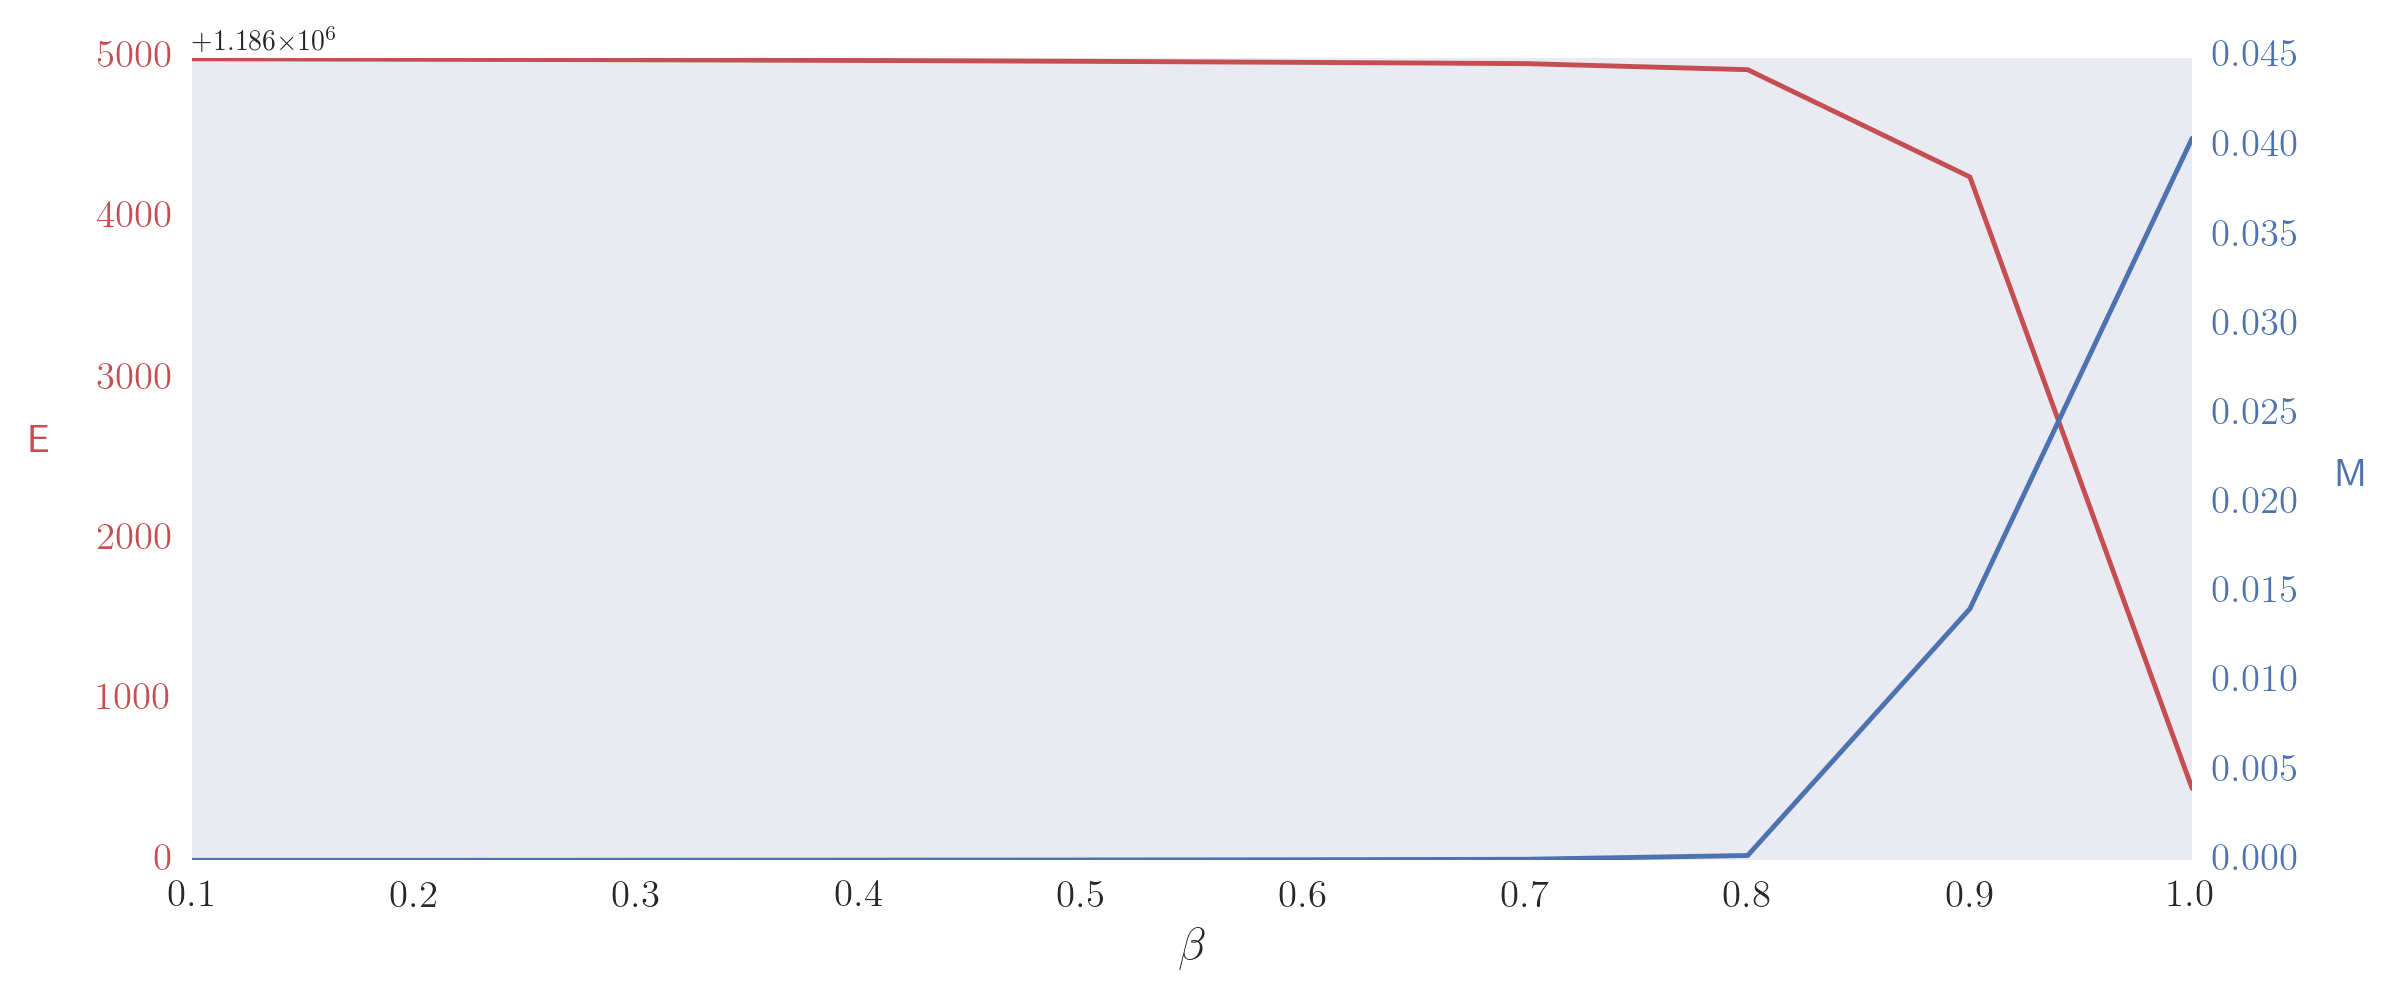
\includegraphics[width=\linewidth]{img/ising-energy-magnetization.png}
% }
% \caption{Energy (E) and magnetization (M) if the Ising spin model with
%   respect to the hyper-parameter $\beta$.}\label{snt:fig:ising-spin-em}
% \end{figure}

\begin{table}[h]
  \begin{center}
    \bgroup \setlength\tabcolsep{0.1\tabcolsep}\scriptsize
    \begin{tabular}{p{0.172\columnwidth} % first columm
        >{\centering\arraybackslash}p{0.06\columnwidth} % second columm
        *{9}{>{\centering\arraybackslash}p{0.07\columnwidth}} % next nine columns
        *{2}{>{\centering\arraybackslash}p{0.053\columnwidth}}} % last two columns
      \toprule
      \multirow{2}*{\bfseries Lexicon} & %
      \multirow{2}{0.06\columnwidth}{\bfseries \# of Terms} & %
      \multicolumn{3}{c}{\bfseries Positive Expressions} & %
      \multicolumn{3}{c}{\bfseries Negative Expressions} & %
      \multicolumn{3}{c}{\bfseries Neutral Terms} & %
      \multirow{2}{0.068\columnwidth}{\bfseries\centering Macro\newline \F{}} & %
      \multirow{2}{0.068\columnwidth}{\bfseries\centering Micro\newline \F{}}\\
      \cmidrule(lr){3-5}\cmidrule(lr){6-8}\cmidrule(lr){9-11}

      & & Precision & Recall & \F{} & %
      Precision & Recall & \F{} & %
      Precision & Recall & \F{} & & \\\midrule
      %% \multicolumn{9}{|c|}{\cellcolor{cellcolor}Existing Lexicons}\\\hline

      % Class                     Precision              Recall                 F-score
      % positive                   0.770601             0.101975                 0.180115
      % negative                   0.567901             0.017139                 0.033273
      % neutral                    0.963176             0.999227                 0.980870
      % Macro-average              0.767226             0.372780                 0.398086
      % Micro-average              0.962404             0.962216                 0.962310

      \textsc{Seed Set} & 20 & \textbf{0.771} & 0.102 & 0.18 & %
      \textbf{0.568} & 0.017 & 0.033 & %
      0.963 & \textbf{0.999} & \textbf{0.981} & %
      0.398 & \textbf{0.962}\\

      % Class                     Precision              Recall                 F-score
      % positive                   0.646220             0.133510                 0.221299
      % negative                   0.565217             0.029061                 0.055280
      % neutral                    0.964071             0.998134                 0.980807
      % Macro-average              0.725169             0.386902                 0.419129
      % Micro-average              0.962261             0.962072                 0.962167

      TKM & 920 & 0.646 & \textbf{0.134} & \textbf{0.221} & %
      0.565 & \textbf{0.029} & \textbf{0.055} & %
      \textbf{0.964} & 0.998 & \textbf{0.981} & %
      \textbf{0.419} & \textbf{0.962}\\

      % Class                     Precision              Recall                 F-score
      % positive                   0.764317             0.102269                 0.180400
      % negative                   0.567901             0.017139                 0.033273
      % neutral                    0.963181             0.999199                 0.980860
      % Macro-average              0.765133             0.372869                 0.398178
      % Micro-average              0.962384             0.962196                 0.962290

      VEL & 60 & 0.764 & 0.102 & 0.18 & %
      \textbf{0.568} & 0.017 & 0.033 & %
      0.963 & 0.999 & 0.98 & %
      0.398 & \textbf{0.962}\\

      % Class                     Precision              Recall                 F-score
      % positive                   0.386437             0.105806                 0.166127
      % negative                   0.567901             0.017139                 0.033273
      % neutral                    0.963178             0.996092                 0.979359
      % Macro-average              0.639172             0.373012                 0.392920
      % Micro-average              0.959478             0.959290                 0.959384

      KIR & 320 & 0.386 & 0.106 & 0.166 & %
      \textbf{0.568} & 0.017 & 0.033 & %
      0.963 & 0.996 & 0.979 & %
      0.393 & 0.959\\

      % Class                     Precision              Recall                 F-score
      % positive                   0.679764             0.101975                 0.177345
      % negative                   0.567901             0.017139                 0.033273
      % neutral                    0.963162             0.998820                 0.980667
      % Macro-average              0.736942             0.372644                 0.397095
      % Micro-average              0.962013             0.961825                 0.961919

      SEV & 60 & 0.68 & 0.102 & 0.177 & %
      \textbf{0.568} & 0.017 & 0.033 & %
      0.963 & \textbf{0.999} & \textbf{0.981} & %
      0.397 & \textbf{0.962}\\

      TKM $\cap$ VEL $\cap$ SEV & 20 & \textbf{0.771} & 0.102 & 0.18 & %
      \textbf{0.568} & 0.017 & 0.033 & %
      0.963 & \textbf{0.999} & \textbf{0.981} & %
      0.398 & \textbf{0.962}\\

      % Class                     Precision              Recall                 F-score
      % positive                   0.592689             0.133805                 0.218322
      % negative                   0.565217             0.029061                 0.055280
      % neutral                    0.964063             0.997700                 0.980593
      % Macro-average              0.707323             0.386855                 0.418065
      % Micro-average              0.961850             0.961662                 0.961756

      TKM $\cup$ VEL $\cup$ SEV & 1,020 & 0.593 & \textbf{0.134} & 0.218  & %
      0.565 & \textbf{0.029} & \textbf{0.055} & %
      \textbf{0.964} & 0.998 & 0.98 & %
      0.418 & \textbf{0.962}\\\bottomrule
    \end{tabular}
    \egroup
    \caption{Evaluation of corpus-based approaches.\\ {\small TKM --
        \citet{Takamura:05}, VEL -- \citet{Velikovich:10}, KIR --
        \citet{Kiritchenko:14}, SEV -- \citet{Severyn:15}}}
    \label{snt-lex:tbl:corp-meth}
  \end{center}
\end{table}

The results of this evaluation are shown in
Table~\ref{snt-lex:tbl:corp-meth}.  This time, we can observe a clear
superiority of Takamura et al.'s method, which not only achieves the
best recall and \F{}-value in recognizing positive and negative items
but also attains the highest micro- and macro-averaged results for all
three polarity classes.
% As expected, the best precision in recognizing polar terms is achieved
% by the manually compiled seed set, whose micro-averaged \F{}-result,
% however, is still identical to the one shown by the method of
% \citet{Takamura:05}.
The size and scores of the other lexicons, however, are much smaller
than the cardinalities and results shown by Takamura et al.'s and
dictionary-based approaches.  Moreover, those polarity lists also show
absolutely identical scores for the negative expressions as the
original seed set.  Since these results were somewhat unexpected, we
decided to investigate the reasons for possible problems.  As it
turned out, the macro-averaged \F{}-values of the other methods were
rapidly going down on the held-out development set as the number of
their induced polar terms increased.  Since we considered the lexicon
size as one of the hyper-parameters of the tested approaches, we
rapidly stopped populating these lexicons when we noticed a decrease
in their results.  As a consequence, only the terms with the highest
ranks (all of which had the positive polarity) were included in the
final lists.

A closer look at the data revealed that the positive bias of the
learned lexicons was mainly due to the ambiguity of the seed set:
While converting the original seed list of \citet{Turney:03} to
German, we translated the English word ``correct'' as ``richtig''.
This German word, however, also has another reading which means
\emph{real}---as in ``ein richtiges Spiel'' (\emph{a real game}) or
``ein richtiger Rennwagen'' (\emph{a real sports car})---and which was
much more frequent in the analyzed snapshot, often appearing in a
negative context---e.g., ``ein richtiger Bombenanschlag'' (\emph{a
  real bomb attack}) or ``ein richtiger Terrorist'' (\emph{a real
  terrorist}).  As a consequence of this, methods relying on distant
supervision had to deal with an extremely unbalanced training
set\footnote{The automatically labeled corpus that we obtained for the
  approach by \citet{Kiritchenko:14} using these seeds, for instance,
  had 716,210 positive versus 92,592 negative training instances.} and
fell victim to this unjustified skewness, getting stuck in a local
optimum from the very beginning of their training.  We will
investigate later in Section~\ref{subsec:snt-lex:eoss} whether the
seed sets proposed by other authors could provide a remedy to this
problem.

\subsection{NWE-Based Methods}

Another group of SLG methods that we are going to explore in this
section are algorithms which operate on distributed vector
representations of words---neural word embeddings (NWEs).  Introduced
by~\citet{Bengio:03}, \citet{Collobert:11}, and \citet{Mikolov:13},
NWEs had a great ``tsunami''-like effect on many downstream NLP
applications~\cite{Manning:15} including part-of-speech
tagging~\cite{Collobert:11}, syntactic
parsing~\cite{Kiperwasser:16b,Kiperwasser:16a}, named entity
recognition~\cite{dosSantos:15} etc.  Unfortunately, to this day, the
SLG task remained largely untouched from these advances, up to a few
works introduced by~\citet{Tang:14a} and \citet{Vo:16}.  In the former
method, the authors used a $k$-NN classifier in order to predict the
polarity of hybrid word embeddings (\citeauthor{Tang:14a} considered
the occurrence of positive and negative smileys as noisy sentiment
labels for tweets and incorporated the polarity prediction as an
additional training objective for computing the word vectors).  In the
latter approach, \citet{Vo:16} trained task-specific two-dimensional
embeddings, also utilizing smileys as distantly supervised labels, and
regarded the two elements of each obtained representation as the
positive and negative scores for the respective word.

In order to estimate the potential of these approaches for an
automatic generation of sentiment lexicons for German Twitter, we
reimplemented these methods, extending them to three-way
classification (positive, negative, and neutral), and also came up
with three alternative solutions for obtaining polarity lists from
distributed vector representations of words:
\begin{enumerate}
  \item the method of the nearest centroids,
  \item the principal component analysis,
  \item and the linear projection algorithm.
\end{enumerate}

With the first approach, we used the embeddings of the seed terms to
compute the centroids of the positive, negative, and objective
clusters.  Afterwards, we assigned a new word $w$ to the polarity
group whose centroid was the nearest to the $w$'s vector.  We
considered the distance to the nearest centroid as the polarity score
for the word $w$ and sorted the resulting sentiment lexicon in the
ascending order of these distances.

%% Similarly, with the KNN method, we allocated each new word $w$ to the
%% polarity class $c$ if the seed embeddings of this class appeared more
%% frequently among the neighbors of the $w$'s vector than the seed
%% representations of any other polarity group.

A slightly different technique was used with the approach of the
principal component analysis.  After normally decomposing the
embedding matrix $E$ into its components using SVD:
\begin{align*}
  E = U \Sigma V^T,
\end{align*}
where the matrices $U$ and $V$ represent orthogonal bases of the row
and column spaces of $E$ respectively, we looked for the row axis
$v$,\footnote{Due to implementation specifics, the initial embedding
  vectors had to be represented as columns.} such that the projections
of the embeddings for the seed terms with opposite polarities on this
axis were maximally far apart from each other.

Since PCA, however, was not guaranteed to find the optimum polarity
scale (the orthognal bases of SVD are computed using the covariance
matrix of $E$ and might therefore not capture semantic orientation if
terms with opposite polarities occur in the same contexts), we
additionally introduced our own \emph{linear projection method}, in
which we explicitly adopted this objective: Namely, given two sets of
vectors for the positive and negative seed terms respectively (let us
denote them as $\mathcal{P} = \{\vec{p}_{+_1},\ldots,\vec{p}_{+_m}\}$
and $\mathcal{N} = \{\vec{p}_{-_1},\ldots,\vec{p}_{-_n}\}$), find a
projection line $\vec{b}$ which would maximize the distance between
the projections of terms from these disjoint sets, i.e.: {\small%
\begin{align}
  \small
  \vec{b} &=\argmax\frac{1}{2}\sum_{\vec{p}_+}\sum_{\vec{p}_-}%
  \left\lVert\frac{\vec{b}\cdot\vec{p}_+}{\vec{b}^2}\vec{b}%
  - \frac{\vec{b}\cdot\vec{p}_-}{\vec{b}^2}\vec{b}\right\rVert^2\\
  &=\argmax\frac{1}{2}\sum_{\vec{p}_+}\sum_{\vec{p}_-}\left\lVert\frac{\vec{b}%
    \cdot\left(\vec{p}_{+}-\vec{p}_{-}\right)}{\vec{b}^2}\vec{b}\right\rVert^2,\label{eq:f}%
\end{align}\normalsize}%
where $\frac{\vec{b}\cdot\vec{p}_+}{\vec{b}^2}\vec{b}$ is the
projection of a word embedding with the positive polarity on the line
$\vec{b}$, and $\frac{\vec{b}\cdot\vec{p}_-}{\vec{b}^2}\vec{b}$ is the
respective projection of a negative seed term.\footnote{Since we are
  only interested in finding the slope of the projection line, we
  assume an intercept of zero.}

Considering the $\argmax$ argument in Expression~\ref{eq:f} as our
objective function $f$ to be optimized, we computed the gradient of
this function w.r.t. the projection line $\vec{b}$:

{\small%
  \begin{align}
    \nabla f &= \sum_{\vec{p}_+}\sum_{\vec{p}_-}%
    \gamma\left(\Delta - \gamma\vec{b^{i}}\right),\label{eq:prj-line-grad}%
\end{align}\normalsize}%
where $\Delta$ is the difference between the positive and negative
vectors $\vec{p}_{+}$ and $\vec{p}_{-}$: $\Delta =
\vec{p}_{+}-\vec{p}_{-}$; and $\gamma$ stands for the dot product of
this difference with the projection vector $\vec{b}$ at the $i$-th
iteration step: $\gamma = \Delta \cdot \vec{b}^i$;\footnote{A detailed
  explanation of the gradient computation is given in Appendix~A of
  this paper.} and optimized the line $\vec{b}$ using gradient ascent
until we reached the global maximum of the function $f$.

Afterwards, we projected all known word embeddings on the computed
slope vector and determined the origin $O_{\vec{b}}$ of this vector,
which not necessarily had to be identical with the global origin point
$\vec{0}$ of the initial coordinate system:

{\small%
  \begin{align}
    O_{\vec{b}} &= \mu_- + \frac{\mu_+ - \mu_-}{2},
\end{align}\normalsize}%
where $\mu_-$ is the mean of the projected embeddings of negative seed
terms: $\mu_- = \frac{\sum\vec{p'_-}}{|\mathcal{N}|}$; and $\mu_+$ is
the respective mean for the projections of positive seed words.
Eventually, we created the final list of polar terms, sorting them by
the distance of their projections to the computed origin point in
descending order (so that words whose projections were furthest away
from the central point appeared at the very beginning of the list) and
assigning negative polarity to those terms whose projections were on
the same side from the origin as the negative mean $\mu_-$.

The results of these methods are shown in
Table~\ref{snt-lex:tbl:nwe-meth}:

\begin{table}[h]
  \begin{center}
    \bgroup \setlength\tabcolsep{0.1\tabcolsep}\scriptsize
    \begin{tabular}{p{0.172\columnwidth} % first columm
        >{\centering\arraybackslash}p{0.06\columnwidth} % second columm
        *{9}{>{\centering\arraybackslash}p{0.07\columnwidth}} % next nine columns
        *{2}{>{\centering\arraybackslash}p{0.053\columnwidth}}} % last two columns
      \toprule
      \multirow{2}*{\bfseries Lexicon} & %
      \multirow{2}{0.06\columnwidth}{\bfseries \# of Terms} & %
      \multicolumn{3}{c}{\bfseries Positive Expressions} & %
      \multicolumn{3}{c}{\bfseries Negative Expressions} & %
      \multicolumn{3}{c}{\bfseries Neutral Terms} & %
      \multirow{2}{0.068\columnwidth}{\bfseries\centering Macro\newline \F{}} & %
      \multirow{2}{0.068\columnwidth}{\bfseries\centering Micro\newline \F{}}\\
      \cmidrule(lr){3-5}\cmidrule(lr){6-8}\cmidrule(lr){9-11}

      & & Precision & Recall & \F{} & %
      Precision & Recall & \F{} & %
      Precision & Recall & \F{} & & \\\midrule
      %% \multicolumn{9}{|c|}{\cellcolor{cellcolor}Existing Lexicons}\\\hline

      % Class                     Precision              Recall                 F-score
      % positive                   0.770601             0.101975                 0.180115
      % negative                   0.567901             0.017139                 0.033273
      % neutral                    0.963176             0.999227                 0.980870
      % Macro-average              0.767226             0.372780                 0.398086
      % Micro-average              0.962404             0.962216                 0.962310

      \textsc{Seed Set} & 20 & 0.771 & 0.102 & 0.18 & %
      0.568 & 0.017 & 0.033 & %
      0.963 & 0.999 & 0.981 & %
      0.398 & 0.962\\

      % Class                     Precision              Recall                 F-score
      TNG &  &  &  &  & %
      &  &  & %
      &  &  & %
      & \\

      % Class                     Precision              Recall                 F-score
      VO &  &  &  &  & %
      &  &  & %
      &  &  & %
      & \\

      %% file: 'data/results/ncentroids/ncentroids.word2vec.L.M.turney-littman-seedset.60'

      NC & 60 & 0.771 & 0.102 & 0.18 & %
      0.568 & 0.017 & 0.033 & %
      0.963 & 0.999 & 0.981 & %
      0.398 & 0.962\\

      %% file: 'data/results/knn/knn.word2vec.L.M.turney-littman-seedset.5120'
      %% positive                   0.770601             0.101975                 0.180115
      %% negative                   0.005488             0.017139                 0.008314
      %% neutral                    0.961111             0.942958                 0.951948
      %% Macro-average              0.579067             0.354024                 0.380125
      KNN & 5,120 & 0.771 & 0.102 & 0.18 & %
       0.005 & 0.017 & 0.008 & %
       0.961 & 0.943 & 0.952 & %
       0.38 & 0.908\\

      %% file: ''

      PCA &  &  &  &  & %
       &  &  & %
       &  &  & %
       & \\

      %% file: ''

      LP &  &  &  &  & %
       &  &  & %
       &  &  & %
       & \\\bottomrule
    \end{tabular}
    \egroup
    \caption{Evaluation of NWE-based approaches.\\ {\small
        TNG -- \citet{Tang:14a}, %
        VO -- \citet{Vo:16}, %
        NC --- nearest centroids, %
        KNN --- $k$-nearest neighbors, %
        LP --- linear projection}}%
    \label{snt-lex:tbl:nwe-meth}
  \end{center}
\end{table}

% A new family of lexicon induction methods builds on learned vector
% representations of words -- the neural word embeddings
% \cite{Mikolov:13}.

% Vector command:
% \begin{verbatim}
% Adjusted Potts' Tokenizer

% Sidarenka's Preprocessing (Smiley Replacement)

% word2vec -train tokens.tok -output vectors.txt -size 400 -window 5 -min-count 4

% Possible Improvements:

% * use task specific vectors;

% * decide what to do with smileys during evaluation;

% * explore different cardinalities (not just 40-s bins);
% \end{verbatim}

% % k-NN: k^2 / \sum d_{ij}

% The results of these methods are shown in Table~\ref{snt-lex:tbl:nwe-methods}.

% \begin{table}[h]
%   \begin{center}
%     \bgroup \setlength\tabcolsep{0.1\tabcolsep}\scriptsize
%     \begin{tabular}{p{0.1\columnwidth} % first columm
%         *{9}{>{\centering\arraybackslash}p{0.078\columnwidth}} % next nine columns
%         *{2}{>{\centering\arraybackslash}p{0.078\columnwidth}}} % last two columns
%       \toprule
%           \multirow{2}*{\bfseries Lexicon} & %
%           \multicolumn{3}{c}{\bfseries Positive Expressions} & %
%           \multicolumn{3}{c}{\bfseries Negative Expressions} & %
%           \multicolumn{3}{c}{\bfseries Neutral Terms} & %
%           \multirow{2}{0.068\columnwidth}{\bfseries\centering Macro\newline \F{}} & %
%           \multirow{2}{0.068\columnwidth}{\bfseries\centering Micro\newline \F{}}\\
%           \cmidrule(lr){2-4}\cmidrule(lr){5-7}\cmidrule(lr){8-10}

%           & Precision & Recall & \F{} & %
%           Precision & Recall & \F{} & %
%           Precision & Recall & \F{} & & \\\midrule

%           % cardinality 160
%           NC & 75.7\stddev{23.8} & 9.1\stddev{5.7} & 15.8\stddev{8.8} & %
%           24.4\stddev{41.8} & 1\stddev{1.8} & 1.9\stddev{3.4} & %
%           96.3\stddev{0.8} & \textbf{99.9}\stddev{0.1} & \textbf{98.1}\stddev{0.4} & %
%           38.6\stddev{3.2} & \textbf{96.2}\stddev{0.8}\\

%           % cardinality 40
%           KNN & \textbf{75.8}\stddev{23.8} & 9.1\stddev{5.7} & 15.8\stddev{8.8} & %
%           23.4\stddev{40.6} & 1\stddev{1.8} & 1.8\stddev{3.4} & %
%           96.3\stddev{0.8} & \textbf{99.9}\stddev{0.1} & \textbf{98.1}\stddev{0.4} & %
%           38.6\stddev{3.2} & \textbf{96.2}\stddev{0.8}\\

%           % cardinality 160
%           PCA & 40.4\stddev{14.6} & \textbf{13.4}\stddev{5.8} & \textbf{19.5}\stddev{7.3} & %
%           24.4\stddev{41.8} & 1\stddev{1.8} & 1.9\stddev{3.4} & %
%           \textbf{96.4}\stddev{0.8} & 99.6\stddev{0.2} & 97.9\stddev{0.4} & %
%           39.8\stddev{2.7} & 95.9\stddev{0.8}\\

%           % cardinality 160
%           LP & \textbf{75.8}\stddev{23.8} & 9.1\stddev{5.7} & 15.8\stddev{8.8} & %
%           \textbf{29.4}\stddev{20.3} & \textbf{5.6}\stddev{4.5} & \textbf{9.2}\stddev{6.9} & %
%           \textbf{96.4}\stddev{0.8} & 99.8\stddev{0.1} & 98\stddev{0.4} & %
%           \textbf{41}\stddev{3.9} & 96.1\stddev{0.8}\\
%           \bottomrule
%     \end{tabular}
%     \egroup
%     \caption{Evaluation of embedding-based approaches.\\ {\small (NC
%         -- nearest centroids, KNN -- k-nearest neighbors, PCA --
%         principal component analysis, LP -- linear projection)}}
%     \label{snt-lex:tbl:nwe-methods}
%   \end{center}
% \end{table}

\section{Effect of Seed Sets}\label{subsec:snt-lex:eoss}

An important factor which could significantly affect the quality of
the resulting sentiment lexicons was the set of the seed terms that we
used to initialize the polarity scores of the tested methods.  In
order to estimate the impact of this setting on the final scores, we
re-run our experiments using the seed lists proposed by \citet{Hu:04},
\citet{Kim:04}, \citet{Esuli:06c}, and \citet{Remus:10}.  Since
\citet{Hu:04}, however, only partially specified their seed set in the
original paper, and \citet{Kim:04} did not provide any examples of
their seeds at all, we filled the missing entries in these resources
with common polar German words that we came up with in order to match
the reported size of these lists.  Furthermore, in the cases where the
above seed sets were missing the neutral category, we explicitly added
a number of objective terms proportional to the size of the polar
classes in these lists.  Finally, as the set of neutral terms in the
polarity list of \citet{Esuli:06c} comprised 4,122 words---the authors
considered as neutral all terms from the General Inquirer lexicon
\cite{Stone:66} which were not marked there as either positive or
negative and did not appear in the seed list of
\citet{Turney:03}---and was therefore tedious to translate manually,
we automatically obtained translations for these terms by using the
publicly available online dictionary
\texttt{dict.cc}\footnote{\url{http://www.dict.cc}} and taking the
first suggested German translation for each of the neutral
entries.\footnote{We also tried to use all possible translations of
  the original terms, but it lead to a considerable boost in the
  number of neutral items (45,252 words) and resulted in a substantial
  decrease of the final system scores.} A short statistics on the
cardinality and composition of the resulting seed lists is presented
in Table~\ref{snt-lex:tbl:alt-seed-sets}.

\begin{table}[h]
  \begin{center}
    \bgroup \setlength\tabcolsep{0.1\tabcolsep}\scriptsize
    \begin{tabular}{ %
        >{\centering\arraybackslash}p{0.2\columnwidth} % first columm
        *{4}{>{\centering\arraybackslash}p{0.2\columnwidth}}} % next four columns
      \toprule
      {\bfseries Seed Set} & %
      {\bfseries Cardinality} & %
      {\bfseries Parts of Speech} & %
      {\bfseries Examples} & %
      {\bfseries Comments}\\
      \midrule
      \citet{Hu:04} & 14 positive, 15 negative, and 10 neutral terms & adjectives %
      & {{\itshape fantastisch, lieb, sympathisch, %
          b\"ose, dumm, schwierig}} & polar terms translated from the original paper %
      \cite{Hu:04}; neutral terms added by us;\\
      \citet{Kim:04} & 60 positive, 60 negative, and 60 neutral terms & any & %
      {\itshape fabelhaft, Hoffnung, lieben, h\"asslich, Missbrauch, t\"oten} %
      & devised by us so as to match the cardinality of the original set with %
      neutral terms added extra;\\
      \citet{Esuli:06c} & 16 positive, 35 negative, and 4,122 neutral terms & %
      any & {\itshape angenehm, ausgezeichnet, freundlich, %
        arm, bedauernswert, d\"urftig} & polar terms translated from the seed %
      set of \citet{Turney:03}; neutral terms automatically translated from %
      objective entries in the General Inquirer lexicon \cite{Stone:66};\\
      \citet{Remus:10} & 12 positive, 12 negative, and 10 neutral terms & %
      adjectives & {\itshape gut, sch\"on, richtig, %
        schlecht, unsch\"on, falsch} & %
      polar terms translated from the seed set of \citet{Turney:03}; %
      neutral terms added by us.\\
      \\\bottomrule
    \end{tabular}
    \egroup
    \caption{Cardinality and composition of the alternative polarity lists.\\
      (all cardinalities are given with respect to the resulting
      German translations)}
    \label{snt-lex:tbl:alt-seed-sets}
  \end{center}
\end{table}

The updated results of the dictionary-based approaches with these
alternative seed sets are shown in
Figure~\ref{snt:fig:sent-dict-lex-alt-seeds}.  This time, we again can
notice superior scores achieved by the method of
\citet{Blair-Goldensohn:08}, which not only outperforms other systems
on average but also seems to be less susceptible to the varying
quality and size of different seeds.  The remaining methods typically
achieve their best macro-averaged \F{}-results with either of the two
top-performing initial polarity lists: the seed set of \citet{Kim:04}
or the seed set of \citet{Esuli:06c}.  The former option works best
for the label-propagation approach of \citet{Rao:09} and the random
walk algorithm of \citet{Awadallah:10}.  Moreover, the results shown
by the min-cut system \cite{Rao:09} and the original method of
\citet{Kim:04} when used with this seed set are only slightly lower
than their respective scores achieved with the best possible
configuration---the seed list of \citet{Turney:02}.  The latter
option---the seed set of \citet{Esuli:06c}---shows best results for
the approaches of \citet{Hu:04} and the \textsc{SentiWordNet} method
of \citet{Esuli:06c}.

\begin{figure}[hbtp!]
  \centering
  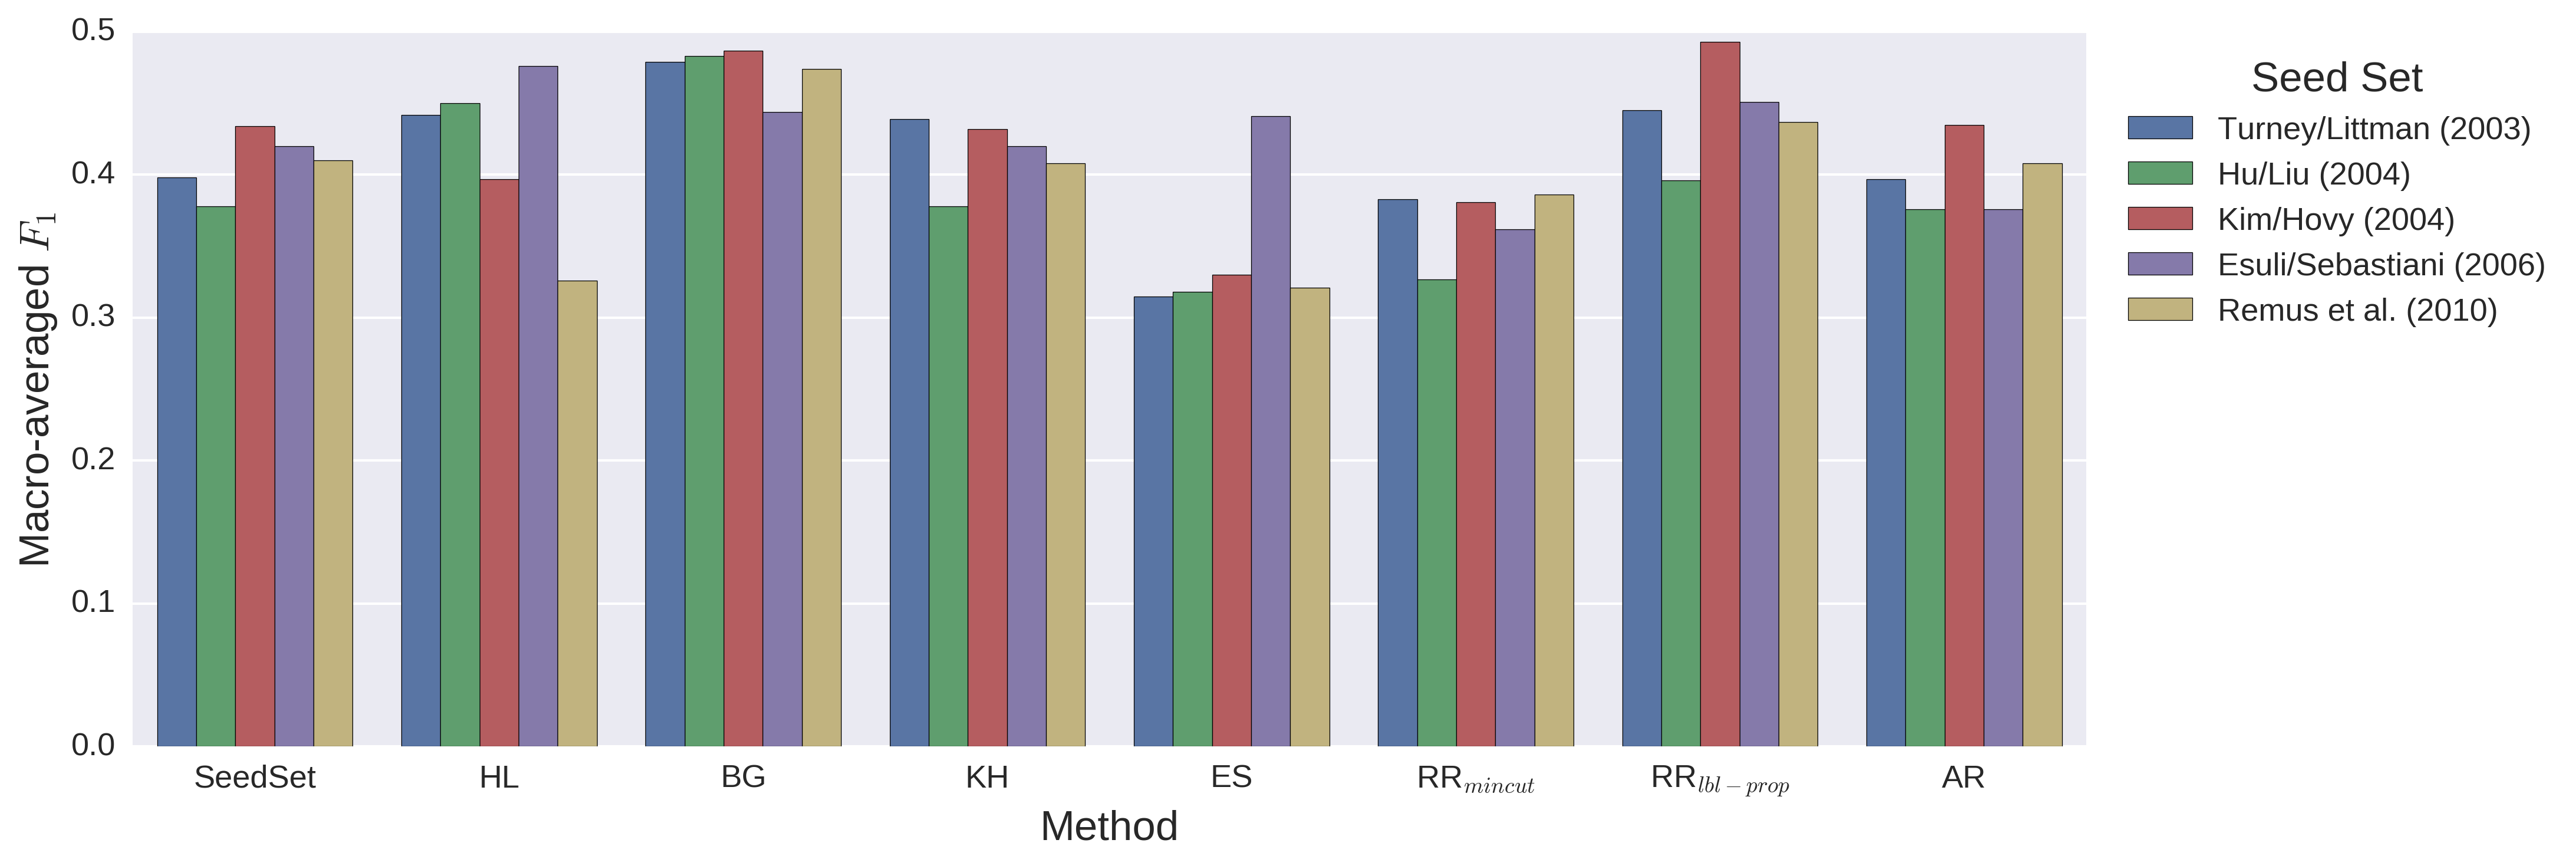
\includegraphics[height=12em,width=\linewidth]{%
    img/sentilex-dict-alt-seed-sets.png}
  \caption{Macro-averaged \F{}-scores of the dictionary-based approaches
    with different seed sets.}\label{snt:fig:sent-dict-lex-alt-seeds}
\end{figure}

A slightly different situation is observed for the corpus-based
approaches as shown in Figure~\ref{snt:fig:sent-crp-lex-alt-seeds}.
Except for the method of \citet{Takamura:05}, which achieves its best
result with the seed set of \citet{Hu:04}, all three remaining
methods---\citet{Velikovich:10}, \citet{Kiritchenko:14}, and
\citet{Severyn:15}---show very similar (though not identical) scores
to the ones reached by the non-expanded seed sets.  The primary reason
for this is again the ambiguity of the translated seeds, which causes
a rapid decrease of the lexicon quality and, consequently, an early
stopping of the expansion.

\begin{figure}[hbtp!]
  \centering
  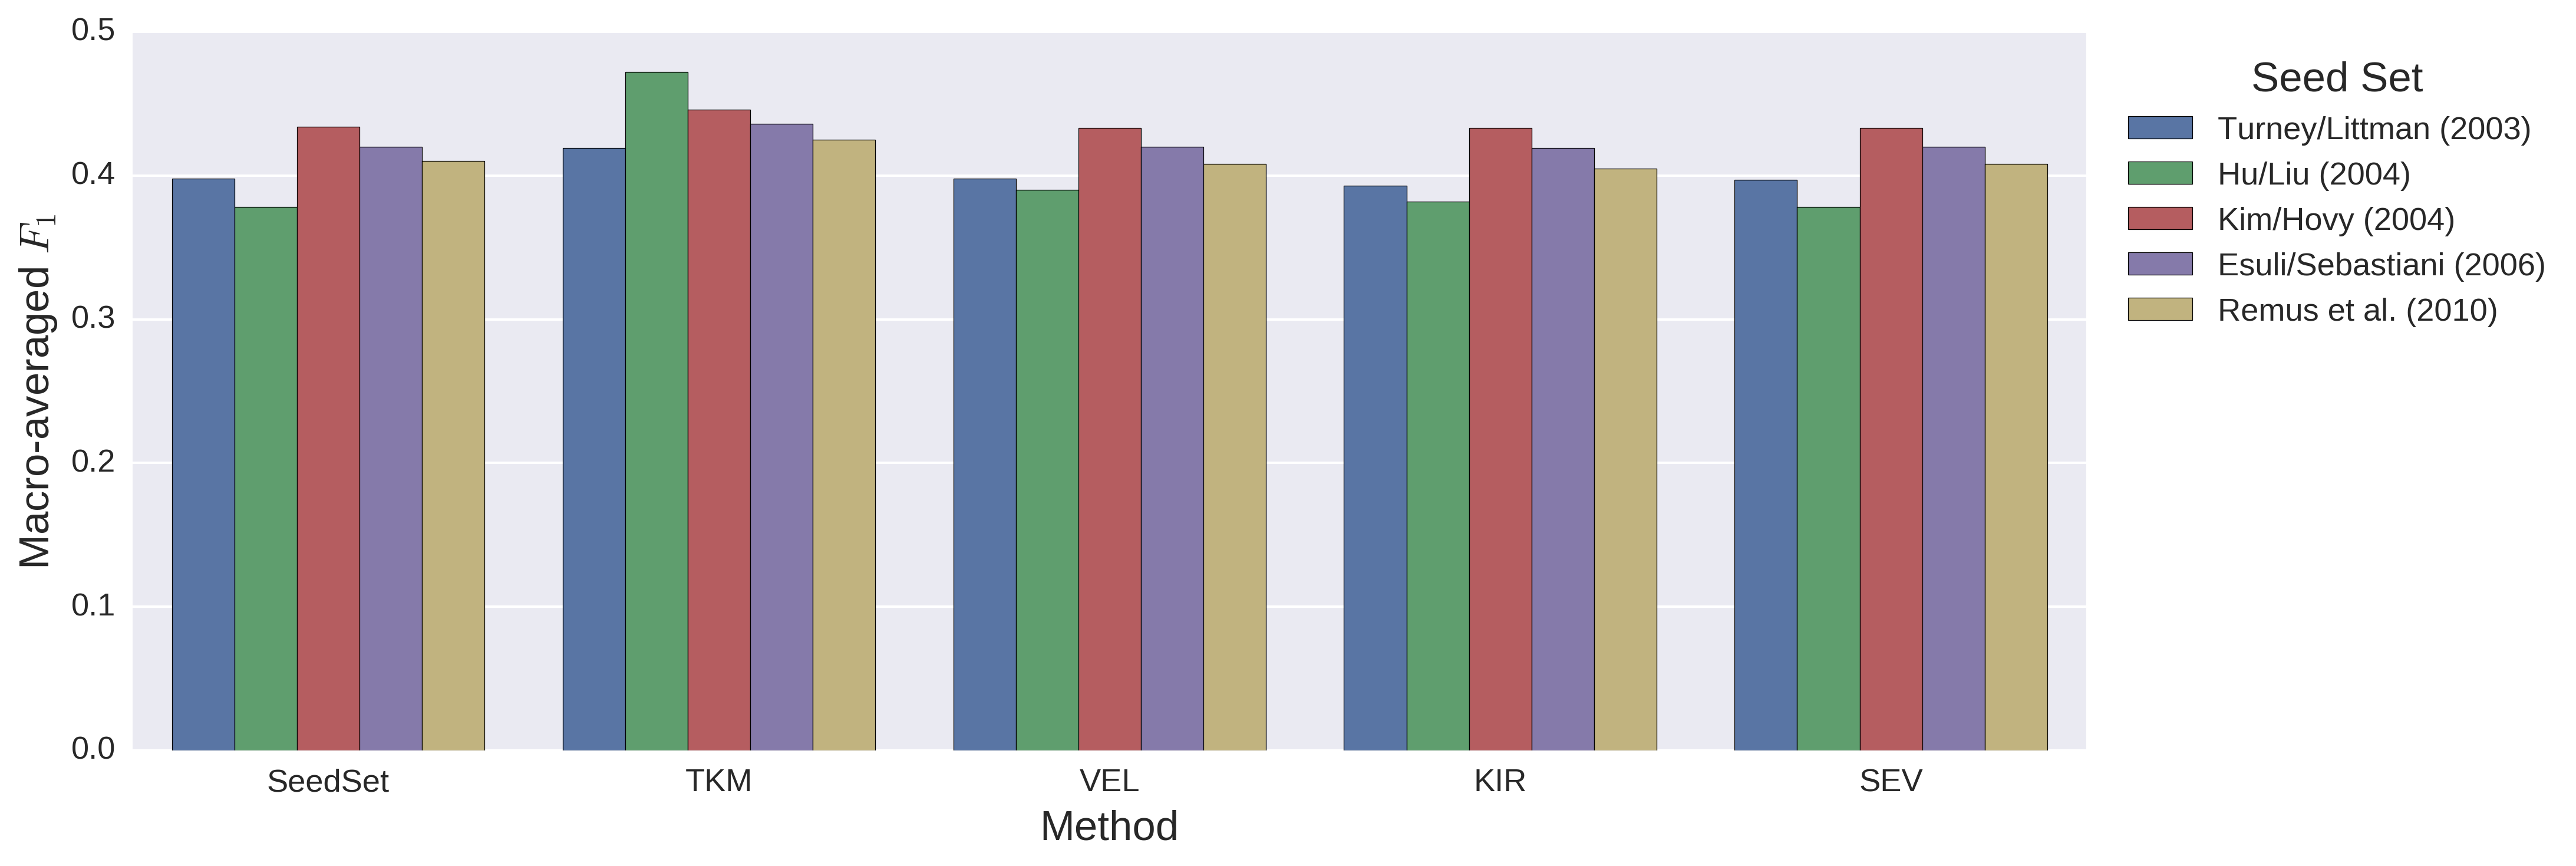
\includegraphics[height=12em,width=\linewidth]{%
    img/sentilex-crp-alt-seed-sets.png}
  \caption{Macro-averaged \F{}-scores of the corpus-based approaches
  with different seed sets.}\label{snt:fig:sent-crp-lex-alt-seeds}
\end{figure}

% For convenience, we will summarize the results of three top-performing
% configurations---the methods of \citet{Blair-Goldensohn:08},
% \citet{Kim:04,Kim:06}, and the label-propagation approach of
% \citet{Rao:09} used in combination with the initial seed sed of
% \citet{Kim:04}---in Table~\ref{snt-lex:tbl:lex-kh-seedset} and use
% these results as baselines in our later experiments.

% \begin{table}[h]
%   \begin{center}
%     \bgroup \setlength\tabcolsep{0.1\tabcolsep}\scriptsize
%     \begin{tabular}{p{0.1\columnwidth} % first columm
%         *{9}{>{\centering\arraybackslash}p{0.078\columnwidth}} % next nine columns
%         *{2}{>{\centering\arraybackslash}p{0.078\columnwidth}}} % last two columns
%       \toprule
%           \multirow{2}*{\bfseries Lexicon} & %
%           \multicolumn{3}{c}{\bfseries Positive Expressions} & %
%           \multicolumn{3}{c}{\bfseries Negative Expressions} & %
%           \multicolumn{3}{c}{\bfseries Neutral Terms} & %
%           \multirow{2}{0.068\columnwidth}{\bfseries\centering Macro\newline \F{}} & %
%           \multirow{2}{0.068\columnwidth}{\bfseries\centering Micro\newline \F{}}\\
%           \cmidrule(lr){2-4}\cmidrule(lr){5-7}\cmidrule(lr){8-10}

%           & Precision & Recall & \F{} & %
%           Precision & Recall & \F{} & %
%           Precision & Recall & \F{} & & \\\midrule

%           BG & 22.7\stddev{6.5} & \textbf{29.9}\stddev{8.4} & 25.4\stddev{6.7} & %
%           17.1\stddev{7.4} & \textbf{16.9}\stddev{7.2} & \textbf{16.6}\stddev{6.7} & %
%           \textbf{97}\stddev{0.6} & 96.4\stddev{0.6} & 96.7\stddev{0.5} & %
%           46.3\stddev{3.5} & 93.5\stddev{0.9}\\

%           KH & 51.6\stddev{12.4} & 21.7\stddev{7.2} & \textbf{29.9}\stddev{8.1} & %
%           38.9\stddev{24.7} & 7.5\stddev{4.9} & 12.2\stddev{7.8} & %
%           96.7\stddev{0.7} & \textbf{99.4}\stddev{0.2} & \textbf{98}\stddev{0.4} & %
%           \textbf{46.7}\stddev{3.9} & \textbf{96}\stddev{0.7}\\

%           RR$_{\textrm{lbl-prop}}$ & \textbf{52.9}\stddev{15.2} & 18.4\stddev{6.5} & 26.7\stddev{8.2} & %
%           \textbf{42.8}\stddev{29.7} & 8.9\stddev{5.8} & 14.1\stddev{8.8} & %
%           96.6\stddev{0.7} & \textbf{99.4}\stddev{0.3} & \textbf{98}\stddev{0.4} & %
%           46.3\stddev{4.3} & \textbf{96}\stddev{0.8}\\
%           \bottomrule
%     \end{tabular}
%     \egroup
%     \caption{Results of the top-scoring dictionary-based approaches
%       with the best observed seed set configuration. {\small (BG --
%         \citet{Blair-Goldensohn:08}, KH -- \citet{Kim:04,Kim:06}, RR
%         -- \citet{Rao:09})}}
%     \label{snt-lex:tbl:lex-kh-seedset}
%   \end{center}
% \end{table}

\section{Effect of Word Embeddings}\label{subsec:snt-lex:eowet}

\begin{table}[thb!]
  \begin{center}
    \bgroup\setlength\tabcolsep{0.1\tabcolsep}%
    \setlength{\belowrulesep}{0pt}\scriptsize
    \begin{tabular}{p{0.15\columnwidth} % first columm
        *{4}{>{\centering\arraybackslash}p{0.2\columnwidth}}} % next four columns
      \toprule
      \multirow{2}*{\bfseries Lexicon} & \multicolumn{4}{c}{\bfseries Embedding Type}\\
      & word2vec & task-specific + word2vec & task-specific + least squares & task-specific\\\midrule
      NC &  &  &  & \\
      KNN &  &  &  & \\
      PCA &  &  &  & \\
      LP &  &  &  & \\\bottomrule

    \end{tabular}\egroup%
    {
      \captionsetup{justification=centering}
      \caption{Macro-averaged
        \F-scores of NWE-based methods depending on the embedding type.\\%
                  {\small\itshape%
                    NC --- nearest centroids, %
                    KNN --- $k$-nearest neighbors, %
                    PCA --- principal component analysis, %
                    LP --- linear projection%
                  }%
      }\label{snt-lex:tbl:emb-eff}
    }
  \end{center}
\end{table}

\section{Analysis of Entries}\label{subsec:snt-lex:aoe}

Besides investigating the effects of different hyper-parameters and
seed sets, we also decided to have a closer look at the actual results
produced by the tested methods.  For this purpose, we extracted ten
highest scored entries (not counting the seed terms) from each
dictionary-based automatic lexicon and summarized them in
Table~\ref{tbl:snt-lex:dict:top-10}.

\begin{table}[h]
  \begin{center}
    \bgroup \setlength\tabcolsep{0.03\tabcolsep}\scriptsize
    \begin{tabular}{%
        >{\centering\arraybackslash}p{0.07\columnwidth} % first columm
        *{6}{>{\centering\arraybackslash}p{0.155\columnwidth}}} % last two columns
      \toprule
      \textbf{Rank} & %
      \textbf{HL} & \textbf{BG} & \textbf{KH} & %
      \textbf{ES} & \textbf{RR}$^{**}_{\textrm{mincut}}$ & %
      \textbf{RR}$_{\textrm{lbl-prop}}$\\\midrule
      1 & \ttranslate{perfekt}{perfect} & %
      \ttranslate{flei\ss{}ig}{diligent} &%
      \ttranslate{anr\"uchig}{indecent} &%
      \ttranslate{namenlos}{nameless} &%
      \ttranslate{planieren}{to plane} &%
      \ttranslate{prunkvoll}{splendid}\\

      2 & \ttranslate{musterg\"ultig}{immaculate} & %
      \ttranslate{b\"ose}{evil} &%
      \ttranslate{unecht}{artificial} &%
      \ttranslate{ruhelos}{restless} &%
      \ttranslate{Erdschicht}{stratum} &%
      \ttranslate{sinnlich}{sensual}\\


      3 & \ttranslate{vorbildlich}{commendable} & %
      \ttranslate{beispielhaft}{exemplary} &%
      \ttranslate{irregul\"ar}{irregular} &%
      \ttranslate{unbewaffnet}{unarmed} &%
      \ttranslate{gefallen}{please} &%
      \ttranslate{pomp\"os}{ostentatious}\\

      4 & \ttranslate{beispielhaft}{exemplary} & %
      \ttranslate{edel}{noble} &%
      \ttranslate{drittklassig}{third-class} &%
      \ttranslate{interesselos}{indifferent} &%
      \ttranslate{Zeiteinheit}{time unit} &%
      \ttranslate{unappetitlich}{unsavory}\\

      5 & \ttranslate{exzellent}{excellent} & %
      \ttranslate{t\"uchtig}{proficient} &%
      \ttranslate{sinnlich}{sensual} &%
      \ttranslate{reizlos}{unattractive} &%
      \ttranslate{Derivat}{derivate} &%
      \ttranslate{befehlsgem\"a\ss{}}{as ordered}\\

      6 & \ttranslate{exzeptionell}{exceptional} & %
      \ttranslate{emsig}{busy} &%
      \ttranslate{unprofessionell}{unprofessional} &%
      \ttranslate{w\"urdelos}{undignified} &%
      \ttranslate{Oberfl\"ache}{surface} &%
      \ttranslate{vierschr\"otig}{beefy}\\

      7 & \ttranslate{au\ss{}ergew\"ohnlich}{extraordinary} & %
      \ttranslate{eifrig}{eager} &%
      \ttranslate{abgeschlagen}{exhausted} &%
      \ttranslate{absichtslos}{unintentional} &%
      \ttranslate{Essbesteck}{cutlery} &%
      \ttranslate{regelgem\"a\ss}{regularly}\\

      8 & \ttranslate{au\ss{}erordentlich}{exceptionally} & %
      \ttranslate{arbeitsam}{hardworking} &%
      \ttranslate{gef\"allig}{pleasing} &%
      \ttranslate{ereignislos}{uneventful} &%
      \ttranslate{abl\"osen}{to displace} &%
      \ttranslate{wahrheitsgem\"a\ss}{true}\\

      9 & \ttranslate{viertklassig}{fourth-class} & %
      \ttranslate{musterg\"ultig}{exemplary} &%
      \ttranslate{musterg\"ultig}{exemplary} &%
      \ttranslate{regellos}{irregular} &%
      \ttranslate{Musikveranstaltung}{music event} &%
      \ttranslate{fettig}{greasy}\\

      10 & \ttranslate{sinnreich}{ingenious} & %
      \ttranslate{vorbildlich}{commendable} &%
      \ttranslate{unrecht}{wrong} &%
      \ttranslate{fehlerfrei}{accurate} &%
      \ttranslate{Gebrechen}{afflictions} &%
      \ttranslate{lumpig}{shabby}\\\bottomrule
    \end{tabular}
    \egroup
    \caption{Top ten polar terms produced by the dictionary-based methods.\\
      {\small ** -- the min-cut method of \citet{Rao:09} returns an
        unsorted set}}
    \label{tbl:snt-lex:dict:top-10}
  \end{center}
\end{table}

As can be seen from the table, the approaches of \citet{Hu:04},
\citet{Blair-Goldensohn:08}, \citet{Kim:04}, as well as the
label-propagation algorithm of \citet{Rao:09} produce almost perfect
polarity lists.  The \textsc{SentiWordNet} approach of
\citet{Esuli:06c}, however, already features some spurious terms among
its top-scored entries (e.g., ``absichtslos'' \emph{unintentional}).
Finally, the min-cut approach of \citet{Rao:09} returns a set of
mainly objective terms, which, however, is rather due to the fact that
this method performs a cluster-like partitioning of the lexical graph
without actually ranking the words assigned to a cluster.

A different situation is observed for the corpus-based systems as
shown in Table~\ref{tbl:snt-lex:crp:top-10}: The top-scoring polarity
lists returned by all of these approaches not only include many
apparently objective terms but are also difficult to interpret in
general, as they contain a substantial number of slang and advertising
terms (e.g., ``BMKS65'', ``\#gameinsight'', ``\#androidgames'' etc.).
This again supports the hypothesis that an extreme noisiness of the
input domain might pose considerable difficulties to corpus-based
methods.

\begin{table}[h]
  \begin{center}
    \bgroup \setlength\tabcolsep{0.03\tabcolsep}\scriptsize
    \begin{tabular}{%
        >{\centering\arraybackslash}p{0.07\columnwidth} % first columm
        *{4}{>{\centering\arraybackslash}p{0.232\columnwidth}}} % last two columns
      \toprule
      \textbf{Rank} & %
      \textbf{TKM} & \textbf{VEL} & \textbf{KIR} & %
      \textbf{SEV} \\\midrule
      1 & \ttranslate{Stockfotos}{stock photos} &%
      \ttranslate{Wahl\-kampf\-ge\-schenk}{election gift} &%
      \ttranslate{Suchmaschinen}{search engines} &%
      \ttranslate{Scherwey}{Scherwey}\\

      2 & \ttranslate{BMKS65}{BMKS65} &%
      \ttranslate{Or\-dens\-ge\-schich\-te}{order history} &%
      \ttranslate{\#gameinsight}{\#gameinsight} &%
      \ttranslate{krebsen}{to crawl}\\

      3 & \ttranslate{Ziya}{Ziya} &%
      \ttranslate{Indologica}{Indologica} &%
      \ttranslate{\#androidgames}{\#androidgames} &%
      \ttranslate{kaschieren}{to conceal}\\

      4 & \ttranslate{Shoafoundation}{shoah found.} &%
      \ttranslate{Indologie}{Indology} &%
      \ttranslate{Selamat}{selamat} &%
      \ttranslate{Davis}{Davis}\\

      5 & \ttranslate{T1199}{T1199} &%
      \ttranslate{Energieverbrauch}{energy consumption} &%
      \ttranslate{Pagi}{Pagi} &%
      \ttranslate{\#Klassiker}{\#classics}\\

      6 & \ttranslate{Emilay55}{Emilay55} &%
      \ttranslate{Schimmelbildung}{mold formation} &%
      \ttranslate{\#Sparwelt}{\#savingsworld} &%
      \ttranslate{Nationalismus}{nationalism}\\

      7 & \ttranslate{Eneramo}{Eneramo} &%
      \ttranslate{Hygiene}{hygiene} &%
      \ttranslate{\#Seittest}{\#Seittest} &%
      \ttranslate{Kraftstoff}{fuel}\\

      8 & \ttranslate{GotzeID}{GotzeID} &%
      \ttranslate{wasserd}{waterp} &%
      \ttranslate{Gameinsight}{Gameinsight} &%
      \ttranslate{inaktiv}{idle}\\

      9 & \ttranslate{BSH65}{BSH65} &%
      \ttranslate{heizkostensparen}{saving heating costs} &%
      \ttranslate{\#ipadgames}{\#ipadgames} &%
      \ttranslate{8DD}{8DD}\\

      10 & \ttranslate{Saymak.}{Saymak.} &%
      \ttranslate{Re\-fe\-renz\-ar\-chi\-tek\-tu\-ren}{reference architectures} &%
      \ttranslate{Fitnesstraining}{fitness training} &%
      \ttranslate{Mailadresse}{mail address}\\\bottomrule
    \end{tabular}
    \egroup
    \caption{Top ten polar terms produced by the corpus-based methods.}
    \label{tbl:snt-lex:crp:top-10}
  \end{center}
\end{table}

\section{Discussion}

In general, as we can see from the results, all systems tested in this
section performed notably worse than reported in their original
papers.  We can explain this divergence by the following four reasons:
\begin{enumerate}[1\upshape)]
\item the evaluation metrics that we applied in our experiments were
  considerably different from the testing methods used in the previous
  works (we estimated the results on a real-life corpus, counting
  every false positive and false negative match separately, whereas
  the English approaches typically evaluated their results on the
  intersection with the General Inquirer Lexicon \cite{Stone:66},
  omitting false positive matches and therefore artifically boosting
  their scores);
\item both the domain and the language that we addressed in this
  section were apparently more challenging than the standard English
  form for which most of these methods had been developed;
\item the notion of the synonymous relations used for the
  dictionary-based approaches and the set of the initial seed terms
  used by all methods could differ from the original settings of the
  evaluated algorithms;
\item finally, the underlying lexical taxonomy (\textsc{GermaNet}) and
  the snapshot corpus were different from the resources that were
  originally used for training the presented methods.
\end{enumerate}


% Since \textsc{GermaNet}, however, is significantly different from its
% English counterpart, both quantitatively and qualitatively, we should
% first present some key statistics (shown in
% Table~\ref{snt-lex:tbl:germanet-wordnet}) and visualize the synset
% graphs (demonstrated in Figures~\ref{snt-lex:fig:germanet}
% and~\ref{snt-lex:fig:wordnet}) of these lexical databases.

% \begin{table}[h]
%   \begin{center}
%     \bgroup \setlength\tabcolsep{0.1\tabcolsep}\scriptsize \small
%     \begin{tabular}{p{0.15\textwidth} % first columm
%         *{8}{>{\centering\arraybackslash}m{0.085\textwidth}}} % next nine columns
%       \toprule
%       & \multicolumn{2}{c}{\bfseries Noun} & %
%       \multicolumn{2}{c}{\bfseries Verb} & %
%       \multicolumn{2}{c}{\bfseries Adjective} & & \\
%       \multirow{-2}{0.12\columnwidth}{\centering\bfseries Resource} & %
%       Words & Synsets & Words & Synsets & Words & Synsets & %
%       \multirow{-2}{0.085\columnwidth}{\centering\scriptsize\bfseries{}Hy\-pon.\newline{}Rels} & %
%       \multirow{-2}{0.085\columnwidth}{\centering\scriptsize\bfseries{}Anto\-n.\newline{}Rels}\\
%       \midrule

%       \textsc{GermaNet} & 85,662 & 71,575 & 9,340 & 11,026 & 12,890 & 10,645 & %
%       97,712 & 1,741\\
%       \textsc{WordNet}  & 117,798 & 82,115 & 11,529 & 13,767 & 21,479 & 18,156 & %
%       95,322 & 7,394\\
%       \bottomrule
%     \end{tabular}
%     \egroup
%     \caption{Key statistics on \textsc{GermaNet} and
%       \textsc{WordNet}.}
%     \label{snt-lex:tbl:germanet-wordnet}
%   \end{center}
% \end{table}

% \begin{figure*}[htbp!]
% {
% \centering
% \begin{subfigure}{.5\textwidth}
%   \centering
%   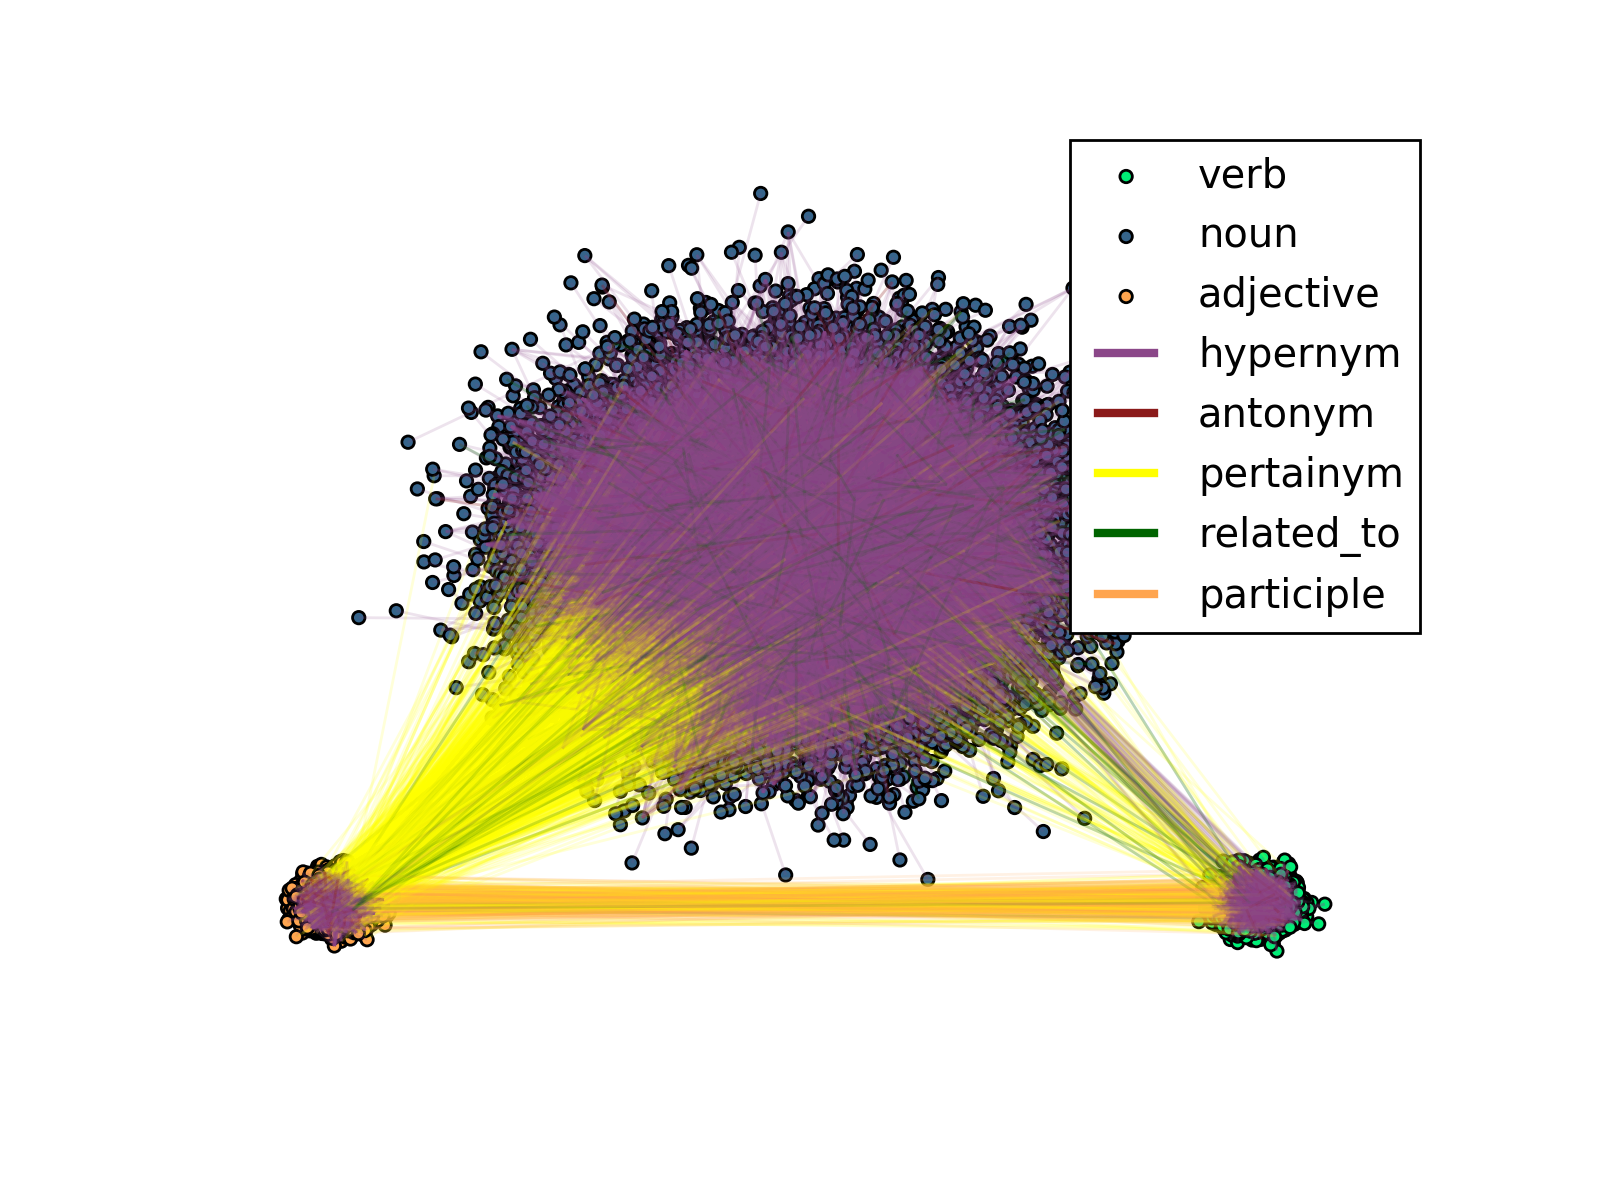
\includegraphics[width=\linewidth]{img/germanet.png}
%   \caption{\textsc{GermaNet}}\label{snt-lex:fig:germanet}
% \end{subfigure}%
% \begin{subfigure}{.5\textwidth}
%   \centering
%   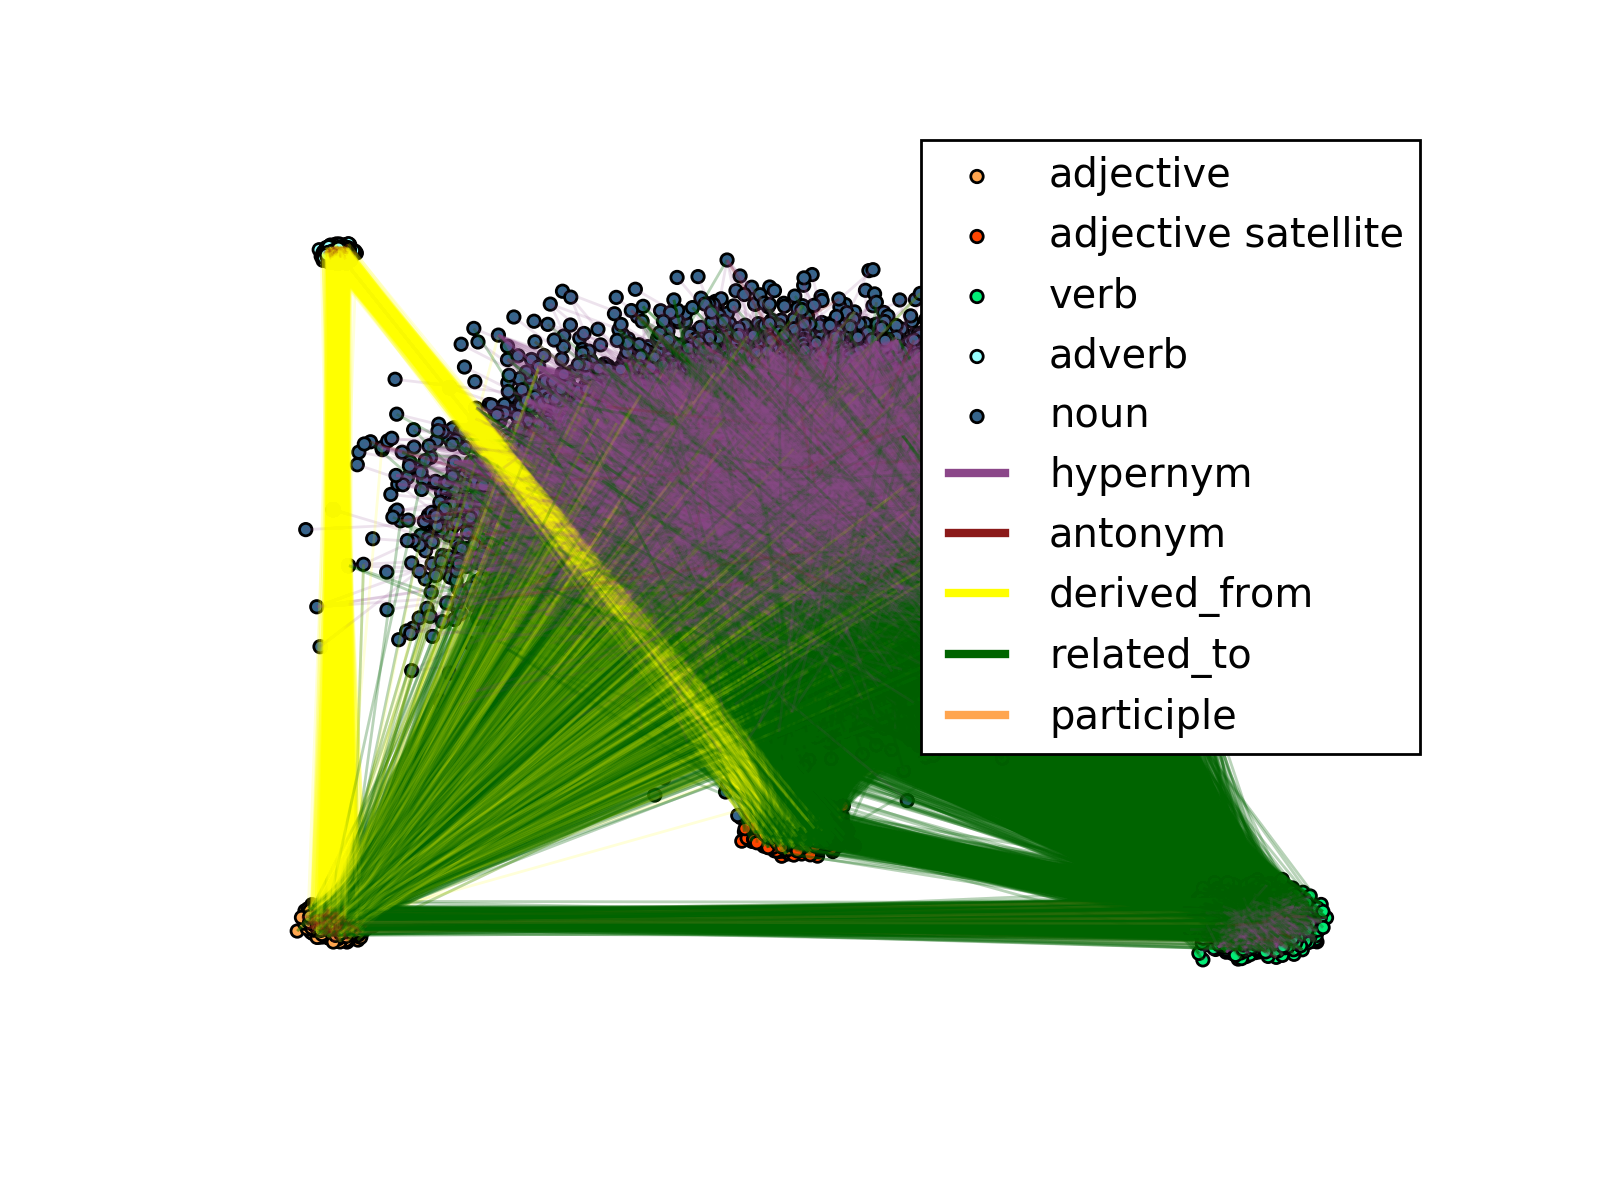
\includegraphics[width=\linewidth]{img/wordnet.png}
%   \caption{\textsc{WordNet}}\label{snt-lex:fig:wordnet}
% \end{subfigure}
% }
% \caption{Graphical visualization of \textsc{GermaNet} and
%       \textsc{WordNet}.}\label{snt:fig:crp-sent-emo-distr}
% \end{figure*}

% As can be seen from the table, \textsc{GermaNet} has significantly
% fewer words and synsets for all common parts of speech with the
% largest gaps observed for nouns and adjectives.  Moreover, as shown in
% Figures~\ref{snt-lex:fig:germanet} and~\ref{snt-lex:fig:wordnet}, such
% PoS-classes as adverbs and adjective satellites are completely missing
% in the German resource.  The reason for this is that the form (and
% meaning) of most German adverbs typically coincides with that of the
% adjectives; therefore, both categories are treated in the same way,
% being represented through the adjectival synsets.

% A slightly different situation can be observed for the semantic links
% (relations) between the synsets: here, \textsc{GermaNet} features
% almost 2,500 more hypernym-hyponym pairs than the English resource,
% whereas the number of antonyms is more than four times less than in
% \textsc{WordNet}.

% An especially interesting pattern, however, appears with the relations
% connecting different parts of speech: As can be seen from the figures,
% the strongest inter-PoS connections in \textsc{GermaNet} are the
% pertainym links between the adjectives and nouns and the participle
% edges between the adjectives and verbs.  The interlinks between the
% nouns and verbs, however, are both much fewer in number and more
% diverse in their nature.  This situation is different in
% \textsc{WordNet} where the prevailing majority of the
% inter-part-of-speech connections are represented through the
% \texttt{related\_to} (especially between the nouns, adjective
% satellites, verbs, and verbs and adjectives) and
% \texttt{derived\_from} links (especially between adverbs and
% adjectives with their satellites).  The relations between the
% adjectives and nouns are mixed though, featuring both
% \texttt{related\_to} and \texttt{derived\_from} connections.  As we
% should see later, these links are crucial for breaking part-of-speech
% dependencies of seed sets in the cases when all seeds belong to the
% same PoS class.

% Another lexical sentiment resource (\textsc{WordNet-Affect}) was
% proposed by \citet{Strapparava:04} who manually compiled a list of
% 1,903 subjective terms and projected these polarities to the
% respective synononyms set in \textsc{WordNet}.  The resulting database
% included 2,874 synsets with a total of 4,787 words.

% \subsection{Domain-Specific Sentiment Lexicons}

% \citet{Chetviorkin:14} obtained a set of possible subjective terms
% from English and Russian microblogs by using an ensemble of supervised
% machine learning classifiers that had previously been trained on a
% manually annotated corpus of movie reviews.  In order to determine the
% prior polarity of the extracted terms, the authors first calculated
% approximate polarity scores of the processed messages using general
% polarity lexicons and then took these rough estimates as prior
% polarity expectations of the candidate expressions.  The posterior
% scores of these expressions were computed using the Ising spin model
% in a similar way to the approach proposed by \citet{Takamura:05}.  The
% resulting lexicon comprised 2,772 words for Russian and 2,786 lexical
% items for English.

\section{Summary and Conclusions}

In this section, we presented a thorough evaluation of the most
popular methods for an automatic generation of sentiment lexicons.
For this purpose, we compared the results achieved by the common
English polarity lists, which were semi-automatically translated into
German, with the scores attained by the original English approaches,
which were applied directly to German data.  In the latter case, we
also juxtaposed automatic dictionary- and corpus-based systems in
order to find out which of these paradigms was better suited for the
inherently noisy Twitter domain.  As many of the corpus-based
algorithms showed an extreme susceptibility to the unbalancedness of
the training sets, we also proposed several novel SLG approaches,
which derived polarity lists by using neural word embeddings trained
on a big unlabeled tweet corpus.  In the concluding step, we analyzed
the effect of different seed sets and hyper-parameters on the net
results of the tested approaches, also explaining possible reasons for
the success and failures of various systems.

Based on our observations and experiments, we can formulate the main
conclusions of this section as follows:
\begin{itemize}
\item semi-automatic translations of common English polarity lists
  notably outperform automatic SLG methods which are applied to German
  data;
\item despite their allegedly worse ability to accommodate new
  domains, dictionary-based approaches are still superior to
  corpus-based systems (at least in terms of an intrinsic evaluation);
\item a potential weakness of the dictionary-based algorithms,
  however, is their dependence on different hyper-parameters and the
  size and composition of the initial seed sets;
\item nevertheless, the effect of the seed sets might be even stronger
  for the corpus-based approaches that rely on distant supervision if
  the resulting noisy labeled training set becomes highly unbalanced;
\item in this regard, NWE-based algorithms might be a much better
  alternative to these methods for capturing domain-specific polar
  words and expressions.
\end{itemize}

\newpage


% FILE: sentiment_fgsa.tex  Version 0.0.1
% AUTHOR: Uladzimir Sidarenka

% This is a modified version of the file main.tex developed by the
% University Duisburg-Essen, Duisburg, AG Prof. Dr. G�nter T�rner
% Verena Gondek, Andy Braune, Henning Kerstan Fachbereich Mathematik
% Lotharstr. 65., 47057 Duisburg entstanden im Rahmen des
% DFG-Projektes DissOnlineTutor in Zusammenarbeit mit der
% Humboldt-Universitaet zu Berlin AG Elektronisches Publizieren Joanna
% Rycko und der DNB - Deutsche Nationalbibliothek

\chapter{Fine-Grained Sentiment Analysis}\label{sec:snt:fgsa}

Even though polar lexicons play a crucial role in opinion-mining
research, they still only serve as a building block for achieving more
challenging and more sophisticated objectives.  One of the most
prominent such objectives is that of fine-grained sentiment analysis
(FGSA), which deals with the identification of subjective evaluative
opinions (\emph{sentiments}), the holders of these opinions
(\emph{sources}), and their respectively evaluated objects
(\emph{targets}) in text.  Since an accurate automatic prediction of
these elements would enable people to track public attitude to
literally any object (e.g., a product, service, or political
decision), FGSA is commonly regarded to be one of the most attractive,
necessary, but, unfortunately, also challenging goals in computational
linguistics.

Researchers usually consider this objective as a sequence labeling
(SL) task, and address it with either of the two popular SL
techniques: conditional random fields (CRFs) or recurrent neural
networks (RNNs).  The former approach represents a discriminative
probabilistic graphical framework, which relies on an extensive set of
hand-crafted features; the latter model utilizes a recursive
computational loop, which can learn feature representations completely
automatically.  In this section, we are going to evaluate each of
these methods in detail in order to find out which of these algorithms
is better suited for the domain of German Twitter.  However, before we
proceed with our evaluation, we should first make a short linguistic
digression and briefly discuss the definition of textual spans, to
which these approaches should assign their labels, and the evaluation
metrics, with which we will estimate the quality of this assignment.

\section{Definition of Sentiment, Target, and Source Spans}
Despite some notable advances and an ongoing active research on
fine-grained opinion extraction, the crucial task of defining the
exact boundaries of sentiment spans and the spans of their respective
targets and sources has not been addressed in the literature with the
due attention yet.  Researchers typically overlook this problem,
leaving its solution to the discretion of their annotators
\cite[cf.][]{Wiebe:05,Klinger:13}.

In contrast to these works, instead of relying on rather intuitive
decisions of our coders, we explicitly provided a rule for determining
opinions' boundaries by telling the experts to assign the
\textsc{sentiment} label to ``\emph{minimal complete syntactic or
  discourse-level units that include both the target of an opinion and
  its actual evaluation}''.

% According to this instruction, during the annotation, linguists first
% had to identify evaluated objects (targets) in text, then find the
% respective evaluative expressions of these objects (usually but not
% necessarily polar terms), and, finally, determine the smallest
% syntactic components (typically noun or verb phrases) or discourse
% units (clauses or sentences) where both of these entities appeared
% together.

A sample annotation analyzed in compliance with this rule is shown in
Example~\ref{snt:fgsa:exmp:sent-anno1}:
\begin{example}[Annotation of a Sentiment Span]\label{snt:fgsa:exmp:sent-anno1}
  \upshape\sentiment{Der neue Papst gilt als
    bescheidener, zur\"uckgenommener Typ.}\\[0.8em]
  \noindent\sentiment{The new Pope is believed to be a sober, modest
    man.}
\end{example}
\noindent In this sentence, an expert had to label the complete clause
as a sentiment, since this unit was the minimal syntactic constituent
which included both the object of the evaluation---``der neue Papst''
(\textit{the new pope})---and the evaluation itself---``bescheidener,
zur\"uckgenommener Typ'' (\textit{a sober, modest man}).

We applied the same principles of minimality and completeness to the
annotation of targets and sources, requiring the main components of
these elements (typically nouns or verbs) to be labeled along with all
their syntactic dependents.  Accordingly, the correct annotation of
the target in the previous example had to look as follows:
\begin{example}[Annotation of a Target Span]\label{snt:fgsa:exmp:sent-anno2}
  \upshape\sentiment{\target{Der neue Papst} gilt als
    bescheidener, zur\"uckgenommener Typ.}\\[0.8em]
  \noindent\sentiment{\target{The new Pope} is believed to be a sober,
    modest man.}
\end{example}
\noindent with the \textsc{target} span assigned to the whole noun
phrase---``der neue Papst'' (\textit{the new pope})---and not only its
main word.

Similarly, source elements had to cover complete syntactic structures
as shown in Example~\ref{snt:fgsa:exmp:src-anno1}:
\begin{example}[Annotation of a Source Span]\label{snt:fgsa:exmp:src-anno1}
  \upshape\sentiment{Die Homosexuellenehe war f\"ur \source{den Kardinal, der jetzt Papst ist,} eine Zerst\"orung von Gottes Plan}\\[0.8em]
  \noindent\sentiment{For \source{the cardinal, who is the Pope now,}
    the same-sex marriage was a destruction of God's plan.}
\end{example}
\noindent This time, again, the whole noun phrase including the
dependent attributive clause---``den Kardinal, der jetzt Papst ist,''
(\textit{the cardinal, who is the Pope now,})---had to be labeled with
the \textsc{source} tag because this constituent was the only
\emph{minimal complete} syntactic node which encompassed both the
immediate holder of the opinion---``Kardinal'' \textit{cardinal}---and
its grammatical dependents, without including any of its parental
elements.

\section{Evaluation Metrics}
The next question which naturally arose after defining the span
boundaries for human coders was that of the best way to compare these
spans with automatically assigned labels.  One possibility to estimate
the quality of such automatic assignment was to compute the precision,
recall, and \F{}-scores using either the binary overlap or exact match
metrics \cite[cf.][]{Choi:06,Breck:07} .  The former method considers
an automatically labeled span as correct if it has at least one token
in common with a labeled entity from the gold annotation.  The latter
metric only regards as true positives those automatic spans which have
absolutely identical boundaries with the expert's assignment.
Unfortunately, both of these approaches are problematic to some
extent: While the binary overlap might be overly optimistic, always
assigning perfect scores to automatic spans which cover the whole
sentence; the exact match metric might, vice versa, be too drastic,
considering the whole assignment as false if only one (possibly
irrelevant) token is missing.

Instead of relying on these measures, we opted for the ``golden mean''
solution to this problem that was proposed by \citet{Johansson:10a}.
In their work, the authors introduced another way of estimating the
quality of automatic label assignments, in which they penalized the
predicted spans proportionally to the number of tokens whose labels
were different from the gold annotation.  More precisely, given a set
of manually annotated entities $\mathcal{S}$ and automatically tagged
spans $\widehat{\mathcal{S}}$, they estimated the precision of an
automatic assignment as:
\begin{equation}\label{eq:fgsa:jmmetric}
  P(\mathcal{S}, \widehat{\mathcal{S}}) = \frac{C(\mathcal{S},
    \widehat{\mathcal{S}})}{|\widehat{\mathcal{S}}|},
\end{equation}
where $C(\mathcal{S},\widehat{\mathcal{S}})$ stands for the \emph{span
  coverage} metric, which is computed as the proportion of overlapping
tokens across all pairs of manually ($s_i$) and automatically ($s_j$)
annotated entities:
\begin{equation*}
  C(\mathcal{S}, \widehat{\mathcal{S}}) = \sum_{s_i \in
    \mathcal{S}}\sum_{s_j \in \widehat{\mathcal{S}}}c(s_i, s_j),
\end{equation*}
and the $|\widehat{\mathcal{S}}|$ term denotes the total number of
spans automatically labeled with the given tag.  Similarly to that,
the recall of the assignment is estimated as:
\begin{equation*}
  R(\mathcal{S}, \widehat{\mathcal{S}}) = \frac{C(\mathcal{S},
    \widehat{\mathcal{S}})}{|\mathcal{S}|},
\end{equation*}
and the \F{}-measure is normally computed as the harmonic mean of the
precision and recall scores:
\begin{equation*}
  F_1 = 2\times\frac{P \times R}{P + R}.
\end{equation*}

Since this proportional estimation could adequately accommodate both
extrema of an automatic annotation---too long and too short
spans---and also penalized for erroneous labels, we decided to use
this measure throughout our subsequent experiments.

\section{Data Preparation}\label{snt:fgsa:subsec:data}

In order to evaluate the CRF and RNN approaches on our data set, we
split the whole corpus into three parts, using 70\% of it as training
data, 10\% as a development set, and the remaining 20\% as a test
corpus.  We tokenized all tweets with an adjusted version of the
Christopher Potts'
tokenizer,\footnote{\url{http://sentiment.christopherpotts.net/code-data/happyfuntokenizing.py}}
and preprocessed them using the rule-based normalization technique of
\citet{Sidarenka:13}.
%% During the normalization, Twitter-specific phenomena like @-mentions,
%% retweets, and URIs that were not syntactically integrated in any
%% sentence of the message were removed from the tweets and those
%% elements which played an integral syntactic role were replaced with
%% the special artificial tokens \%User, \%Link etc.  Emoticons like :-),
%% \smiley{}, \frownie{} etc. were also replaced with the placeholders
%% \%PosSmiley, \%NegSmiley, or simply \%Smiley depending on their prior
%% polarity.  Furthemore, out-of-vocabulary words which could be
%% converted to in-vocabulary terms with a pre-defined set of
%% transformations were also normalized.
Afterwards, we labeled the preprocessed data with their part-of-speech
tags using \texttt{TreeTagger}\footnote{We used \texttt{TreeTagger}
  Version 3.2 with the German parameter file UTF-8.} \cite{Schmid:95},
and parsed the resulting sentences with the \texttt{Mate} dependency
parser\footnote{We used \texttt{Mate} Version \texttt{3.61} with the
  German parameter model 3.6.}  \cite{Bohnet:13}.  Finally, since
\texttt{MMAX2} did not provide a straightforward support for the
character offsets of the annotated tokens, and the automatically
tokenized data could disagree with the original corpus tokenization,
we aligned manual annotation with the automatically split words using
the Needleman-Wunsch alignment algorithm~\cite{Needleman:70}.

\section{Fine-Grained Sentiment Analysis with Conditional Random
  Fields}

The first method that we evaluated on the obtained data was that of
the conditional random fields.  First introduced by
\citet{Lafferty:01}, CRFs had rapidly grown in popularity, turning
into one of the most commonly used probabilistic frameworks, which had
been dominating the NLP field for more than a decade.

The main reasons for the huge success of this model are:
\begin{enumerate}[1)]
\item the \emph{structural nature} of CRFs, which, in contrast to
  single-entity classifiers such as logistic regression or SVM, make
  their predictions over a sequence of covariates, trying to find the
  most likely label assignment for the whole input chain and not only
  its individual elements;
\item the \emph{discriminative power} of this framework, which, in
  contrast to generative probabilistic models such as HMM
  \cite{Rabiner:86}, optimizes the conditional probability
  $P(\boldsymbol{Y}|\boldsymbol{X})$ instead of maximizing the joint
  distribution $P(\boldsymbol{X},\boldsymbol{Y})$ and consequently can
  efficiently deal with overlapping and correlated features;
\begin{example}[Overlapping and Correlated Features]
  In order to demonstrate the different effects of correlated and
  overlapping features on generative and discriminative models, let us
  go through an example where we need to predict whether a tweet
  mentioning ``Merkel'' and ``Steinmeier'' is about the Christian
  Democratic Union (\texttt{CDU}) or Social Democratic Party of
  Germany (\texttt{SPD}).

  As features for this task, we will use lexical unigrams appearing in
  the training data.  Assuming that our training set consists of three
  messages mentioning ``Merkel'' and one microblog mentioning
  ``Steinmeier'' which are labeled as \texttt{CDU}, plus one tweet
  mentioning ``Merkel'' and three posts mentioning ``Steinmeier''
  which are annotated as \texttt{SPD}, the generative Na\"{i}ve Bayes
  model would estimate the probability of the two competing classes
  as:
  \begin{align*}
    P(\mathbf{x}, CDU) =& P(\textrm{Merkel},\textrm{Steinmeier}|CDU)\times P(CDU)\\
    =& P(\textrm{Merkel}|CDU)\times P(\textrm{Steinmeier}|CDU) \times P(CDU)\\
    =&\frac{3}{4}\times\frac{1}{4}\times\frac{4}{8}\approx 0.0938\\
    P(\mathbf{x}, SPD) =& P(\textrm{Merkel},\textrm{Steinmeier}|SPD)\times P(SPD)\\
    =& P(\textrm{Merkel}|SPD)\times P(\textrm{Steinmeier}|SPD) \times P(SPD)\\
    =&\frac{1}{4}\times\frac{3}{4}\times\frac{4}{8}\approx 0.0938.\\
  \end{align*}
  After normalizing these probabilities, we would get equal 50\%
  chances for each of the parties, which is fair regarding the token
  distribution in our corpus.  However, if we replace ``Merkel'' with
  ``von der Leyen'' both in the training data and test example and
  rerun this experiment once again, the probability would get
  significantly skewed towards the CDU class:
  \begin{align*}
    P(\mathbf{x}, CDU) =& P(\textrm{von},\textrm{der},\textrm{Leyen},\textrm{Steinmeier}|CDU)\times P(CDU)\\
    =& P(\textrm{von}|CDU)\times P(\textrm{der}|CDU)\times P(\textrm{Leyen}|CDU)\\
    &\times P(\textrm{Steinmeier}|CDU) \times P(CDU)\\
    =&\frac{3}{4}\times\frac{3}{4}\times\frac{3}{4}\times\frac{1}{4}\times\frac{4}{8}\approx 0.0527\\
    P(\mathbf{x}, SPD) =& P(\textrm{von},\textrm{der},\textrm{Leyen},\textrm{Steinmeier}|SPD)\times P(SPD)\\
    =& P(\textrm{von}|SPD)\times P(\textrm{der}|SPD)\times P(\textrm{Leyen}|SPD)\\
    &\times P(\textrm{Steinmeier}|SPD) \times P(SPD)\\
    =&\frac{1}{4}\times\frac{1}{4}\times\frac{1}{4}\times\frac{3}{4}\times\frac{4}{8}\approx 0.0059,\\
  \end{align*}
  which, after normalization, would result in 90\% chances for
  \texttt{CDU}, and a 10\% score for \texttt{SPD}, even though we only
  changed the name of the politician.

  A different situation can be observed for discriminative models such
  as maximum entropy classifier: Instead of optimizing the joint
  distribution $P(\mathbf{x}, y)$ as it is done by generative
  frameworks, discriminative systems seek to optimize the conditional
  likelihood $P(y|\mathbf{x})$ by maximizing the total probability of
  the training set $\sum_{i=1}^N\log P(y_i|\mathbf{x}_i, \mathbf{w})$.
  This probability is usually estimated using the sigmoid function
  $\frac{1}{1 + e^{-(\mathbf{x}_i, \mathbf{w})}}$, where
  $\mathbf{x}_i$ denotes the input features of the $i$-th training
  instance, and the vector $\mathbf{w}$ stands for the respective
  weights of these features.  By optimizing this function using
  gradient descent, we will arrive at the optimal solution
  $w_1 \approx 0.5$ for the feature ``Merkel'' and $w_2 \approx -0.5$
  for the feature ``Steinmeier'' for the first example, which would
  again result in equal 50\% chances for both classes.  In the second
  example, however, all three features ``von'', ``der'', and ``Leyen''
  would get an equal weight of $\approx 0.3$, and the ``Steinmeier''
  feature would receive a coefficient of $\approx -0.4$, which would
  result in 60\% probability for the test message being about the CDU,
  and 40\% that the tweet is about the SPD.  Even though this still
  means a slight skewness towards \texttt{CDU}; this time, the effect
  of correlated features is much less dramatic than in the generative
  case.
\end{example}
\item and, finally, the \emph{avoidance of the label bias problem},
  which other discriminative classifiers, such as maximum entropy
  Markov networks \cite{McCallum:00}, are known to be susceptible to.
  \begin{example}[Label Bias Problem]
    The label bias problem arises in the cases where a locally optimal
    decision outweighs globally superior solutions.  Consider, for
    example, the sentence ``Aber gerade Erwachsene haben damit
    Schwierigkeiten.'' (\textit{But especially adults have
      difficulties with it.}), for which we need to compute the most
    probable sequence of part-of-speech tags.

    \begin{center}
      \begin{tikzpicture}[node distance=5cm]
        \tikzstyle{tag}=[circle split,draw=gray!50,%
          minimum size=2.5em,inner ysep=2,inner xsep=0,%
          circle split part fill={yellow!20,blue!30}]
      \tikzstyle{word}=[draw=none,inner sep=10pt]

      \node[word] (A) at (1, 1) {Aber};
      \node[tag] (B) at (1, 3) {\footnotesize KON \nodepart{lower} 1.};
      \node[word] (D) at (3, 1) {gerade};
      \node[tag] (E) at (3, 2) {\footnotesize ADJA \nodepart{lower} .5};
      \node[tag] (F) at (3, 4) {\footnotesize ADV \nodepart{lower} .5} ;
      \node[word] (G) at (7, 1) {Erwachsene};
      \node[tag] (I) at (7,2) {\footnotesize ADJA \nodepart{lower} .5} ;
      \node[tag] (H) at (7,4) {\footnotesize NN \nodepart{lower} .5};
      \node[word] (J) at (9,1) {haben};
      \node[tag] (K) at (9,3) {\footnotesize VA \nodepart{lower}\small 1.};
      \node[word] (J) at (11,1) {\ldots};

      \path [-] (B) edge node[below] {$.5$} (E);
      \path [-] (B) edge node[above] {$.5$} (F);

      \path [-] (E) edge node[below] {$.3$} (I);
      \path [-] (E) edge node[below left=0.4] {$.7$} (H);
      \path [-] (F) edge node[above left=0.4] {$.8$} (I);
      \path [-] (F) edge node[above] {$.2$} (H);

      \path [-] (I) edge node[below] {$.1$} (K);
      \path [-] (H) edge node[above] {$.9$} (K);
    \end{tikzpicture}
    \captionof{figure}{\emph{Feature weights for states and
        transitions of the part-of-speech example.}\label{fig:snt:memm-crf}}
    \end{center}
    Assuming that feature weights are distributed as shown in
    Figure~\ref{fig:snt:memm-crf}, we will first estimate the
    probability of the correct label sequence for the initial part of
    this sentence using the Maximum Entropy Markov Model (MEMM)---the
    predecessor of the conditional random fields.  According to the
    MEMM's definition, the probability of the correct labeling
    ($KON-ADV-NN-VA$) is equal to:
    \begin{align*}
      P(KON, ADV, NN, VA) &= P(KON)\times P(ADV|KON)\\
      &\times P(NN|ADV)\times P(VA|NN)\\
      &=\frac{\exp(1)}{\exp(1)}\times\frac{\exp(0.5 + 0.5)}{\exp(0.5 + 0.5) + \exp(0.5 + 0.5)}\\%
      &\times\frac{\exp(0.2 + 0.5)}{\exp(0.2 + 0.5) + \exp(0.8 + 0.5)}\times\frac{\exp(0.9 + 1.)}{\exp(0.9 + 1.)} \approx 0.177
    \end{align*}
    At the same time, the probability of the incorrect variant
    ($KON-ADV-ADJA-VA$) amounts to $\approx$ 0.323 and will therefore
    be preferred during automatic tagging.

    A different situation is observed with the CRFs, where the
    normalizing factor in the denominator is computed over the whole
    input sequence without factorizing into individual terms for each
    transition as it is done in the MEMM case.  That way, the
    probability of the correct labels would run up to:
    \begin{align*}
      P(KON, ADV, NN, VA) =& P(KON)\times
      P(ADV|KON)\times P(NN|ADV)\\
      &\times P(VA|NN)\\ =&\frac{\exp(1 + 0.5
        \times 3 + 0.2 + 0.9 + 1)}{Z} \approx 0.252,
    \end{align*}
    where
    $Z = \exp(1 + 0.5 \times 3 + 0.2 + 0.9 + 1) + \exp(1 + 0.5 \times
    3 + 0.8 + 0.1 + 1) + \exp(1 + 0.5 \times 3 + 0.7 + 0.9 + 1) +
    \exp(1 + 0.5 \times 3 + 0.3 + 0.1 + 1)$ is the total score of all
    possible label assignments.  The incorrect alternative
    ($KON-ADV-ADJA-VA$), however, would get a probability score of
    $\approx$ 0.207, which is less than the likelihood of the correct
    labeling.
  \end{example}
\end{enumerate}
\textbf{Training} CRFs get these useful properties thanks to a neatly
formulated objective function in which they seek to optimize the
global log-likelihood of the gold labels $\mathbf{Y}$ conditioned on
the training data $\mathbf{X}$.  In particular, given a set of
training instances
$\mathcal{D} = \{(\mathbf{x}^{(n)}, \mathbf{y}^{(n)})\}_{n=1}^N$,
where $\mathbf{x}^{(n)}$ stands for the input variables of the $n$-th
instance, and $\mathbf{y}^{(n)}$ denotes its respective gold labels,
CRF's training adds up to finding feature coefficients $\mathbf{w}$
which maximize the log-probabilities $\ell$ of $\mathbf{y}^{(i)}$
given their covariates $\mathbf{x}^{(i)}$ over the whole corpus:
\begin{equation}\label{snt:fgsa:eq:crf-w}
  \mathbf{w} = \argmax_{\mathbf{w}}\sum_{n=1}^N\ell
  \left(\mathbf{y}^{(n)}|\mathbf{x}^{(n)}\right).
\end{equation}
The likelihood term $\ell(\mathbf{y}^{(n)}|\mathbf{x}^{(n)})$ in this
equation is commonly estimated using a globally normalized softmax
function:
\begin{equation}\label{snt:fgsa:eq:crf-ell}
  \ell\left(\mathbf{y}^{(n)}|\mathbf{x}^{(n)}\right) =
  \ln\left(P(\mathbf{y}^{(n)}|\mathbf{x}^{(n)})\right) =
  \ln\left(\frac{ \exp\left(\sum_{m=1}^{M}\sum_jw_{j} \cdot f_j(x_{m},
    y_{m-1}, y_{m})\right)}{Z}\right),
\end{equation}
where $M$ stands for the length of the $n$-th training instance,
$f_j(x_{m}, y_{m-1}, y_{m})$ denotes the value of the $j$-th feature
function $f$ at the sequence position $m$, $w_j$ represents the
corresponding weight of this feature, and $Z$ is a normalization
factor calculated over all possible label assignments:
\begin{equation}
  Z =
  \sum_{y'\in\mathcal{Y},y''\in\mathcal{Y}}\exp\left(\sum_{m=1}^{M}\sum_jw_{j}
  \times f_j(x_{m}, y'_{m-1}, y''_{m})\right).
\end{equation}
Since this normalizing term appears in the denominator, and couples
together all feature weights that need to be optimized, it becomes
prohibitively expensive to find the best solution to
Equation~\ref{snt:fgsa:eq:crf-w} analytically with a single shot.  A
possible remedy to this problem is to resort to other optimization
techniques such as gradient descent, in which the weights of features
are successively changed towards the direction of the gradient until
the global minimum of the loss function is reached.

From Equation~\ref{snt:fgsa:eq:crf-ell}, we can see that the partial
derivative of the log-likelihood function $\ell$ w.r.t. a single
feature weight $w_j$ amounts to the following solution:
\begin{equation}
  \frac{\partial}{\partial w_j}\ell =%
  \sum_{n=1}^N\sum_{m=1}^Mf_j(x_{m}, y_{m-1}, y_{m}) -%
  \sum_{n=1}^N\sum_{m=1}^{M}\sum_{y'\in\mathcal{Y},y''\in\mathcal{Y}}f_j(x_{m},%
  y'_{m-1}, y''_{m})P(y',y''|\mathbf{x}^{(n)}),
\end{equation}
which, after dividing both parts of the equation with the constant
term $N$---the size of the corpus---can in turn be transformed into:
\begin{equation}
  \frac{1}{N}\frac{\partial}{\partial w_j}\ell = \E[f_j(\mathbf{x},
  \mathbf{y})] - \E_{\mathbf{w}}[f_j(\mathbf{x}, \mathbf{y})],
\end{equation}
where the first term ($\E[f_j(\mathbf{x}, \mathbf{y})]$) is the
expectation of the feature $f_j$ under the empirical distribution, and
the second term ($\E_{\mathbf{w}}[f_j(\mathbf{x}, \mathbf{y})]$) is
the same expectation under the model's parameters $\mathbf{w}$.  That
way, the optimal solution to the log-likelihood objective in
Equation~\ref{snt:fgsa:eq:crf-ell} is the one, where the model's
expectation of the features matches their (true) empirical expectation
in the corpus.

The marginal probabilities of the features, which are required for
computing their expectation, can be estimated dynamically using the
forward-backward (FB) algorithm \cite{Rabiner:90}, which is a
particular case of the more general belief propagation method
\cite[cf.][p.~81]{Barber:12}.

\noindent\textbf{Inference} Once the optimal feature weights are
learned, one can unproblematically compute the most likely label
assignment for a new instance by using the Viterbi algorithm
\cite{Viterbi:67}, which effectively corresponds to the forward pass
of the FB method with the summation over the alternative preceding
states replaced by the maximum operator (hence the other name for this
algorithm---``max-product'').

\noindent\textbf{Features} A crucial component which accounts for a
huge part of the success (or failure) of a CRF system are feature
attributes which are defined by its developer.

Traditionally, feature functions used in CRFs are divided into
transition- and state-based ones.  The former attributes represent
real- or binary-valued functions
$f(\mathbf{x}, y'', y')\rightarrow\mathbb{R}$ associated with some
data predicate $\phi(\mathbf{x})\rightarrow\mathbb{R}$ and the labels
$y''$ and $y'$.  The value of such attribute at position $m$ in
sequence $\mathbf{x}$ is usually defined as follows:
\begin{equation}
  f(\mathbf{x}_m, y'', y') = \begin{cases} \phi(\mathbf{x}_m), &
    \mbox{if } \mathbf{y}_{m-1} = y''\mbox{ and }\mathbf{y}_{m} =
    y'\\ 0, & \mbox{otherwise;}
  \end{cases}
\end{equation}
where the predicate~$\phi$ typically represents a simple unit
function: $\phi(\mathbf{x}_m)\mapsto 1$, $\forall\mathbf{x}_m$.

In contrast to the ternary transition features, state attributes are
associated with binary predicates, whose output depends on the input
data at the given position and the label $y'$ at the respective state:
\begin{equation}
  f(\mathbf{x}_m, y') = \begin{cases} \phi(\mathbf{x}_m), & \mbox{if }
    \mathbf{y}_{m} = y'\\ 0, & \mbox{otherwise.}
  \end{cases}
\end{equation}
This time, the predicate~$\phi$ is usually much more sophisticated, as
it reflects various properties of the input sequence at the respective
position, such as whether the current token is capitalized or whether
it begins with a specific prefix or ends with a specific suffix.  This
type of features commonly accounts for the overwhelming majority of
all attributes used in a CRF system.

As state attributes in our experiments, we used the following types of
predicates (which, for simplicity, are listed here in groups):
\begin{itemize}
\item\emph{formal}, which included the initial three characters of
  each token (e.g., $\phi_{abc}(\mathbf{x}_m) = 1\mbox{ if
  }\mathbf{x}_m\sim\mbox{ /\textasciicircum abc/ else } 0$), its last
  three characters, and the general spelling class of the token (e.g.,
  alphanumeric, digit, or punctuation);

\item\emph{morphological}, which encompassed the part-of-speech tags
  of the analyzed tokens as well as case and gender values for
  inflectable PoS types, the degree of comparison for adjectives, and
  mood, tense, and person forms for verbs;

\item\emph{lexical}, which comprised the actual lemma and form of the
  tokens (using one-hot encoding), their polarity classes (positive,
  negative, or neutral), which we obtained from the Zurich Polarity
  Lexicon~\cite{Clematide:10};

\item and, finally, \emph{syntactic}, which included the dependency
  relation via which token $x_m$ was connected to its parent; two
  binary features reflecting whether the previous token in the sentence
  was the parent or child of the current word; as well as two other
  features, one of which encoded the dependency relation of the
  previous token in the sentence to its parent + dependency relation
  of the current token to its ancestor, and the other reflected the
  dependency link of the next token + dependency relation of the
  current token to its parent.
\end{itemize}

In addition to the above attributes, we also used a set of complex
lexico-syntactic features, which simultaneously combined several
semantic and syntactic traits.  These included:
\begin{itemize}
\item the lemma of the syntactic parent;
\item the part-of-speech tag and the polarity class of the
  grandparent;
\item the lemma of the child node + dependency relation connecting the
  parent with this child;
\item the PoS tag of the child node + its dependency relation + PoS
  tag of the current token;
\item the lemma of the child node + its dependency relation + lemma of
  the current token;
\item the overall polarity of the children, which was computed by
  summing up the polarity scores of all immediate syntactic
  descendants, and checking whether the resulting value was greater,
  less than or equal to zero.\footnote{We again used the Zurich
    Polarity Lexicon of~\citet{Clematide:10} for computing these
    scores.}
\end{itemize}

\textbf{Results} The results of our experiments are shown in
Table~\ref{snt-fgsa:tbl:crf-res}.  As we can see from the table, with
the given set of features, the model can perfectly well fit the
training data, achieving a macro-averaged \F-score of~0.904.  The
learned parameters, however, only partially generalize to unseen
tweets, leading to notably lower \F-results on the test corpus
(0.287).  This disbalance indicates a strong ``overfitting'' of the
model to the training data (i.e., the assignment of unreasonably high
weights to rather sporadic, noisy features, which only accidentally
co-occurred with the target classes in the corpus).

Another notable tendency, which can be observed both on the training
and test splits, is that the recall of the CRF system is generally
lower than its precision.  This again can be attributed to the
overfitting effect, due to which, less indicative features become more
important than attributes which actually give rise to subjective
evaluations.  Since the former features might not to appear in the
test data or, even if they do, are unlikely to correlate with the
sentiment entities, the model often fails to recognize sentiments in
new contexts which do have important but underweight traits.

\begin{table*}
  \begin{center}
    \bgroup \setlength\tabcolsep{0.1\tabcolsep}\scriptsize
    \begin{tabular}{p{0.162\columnwidth} % first columm
        *{9}{>{\centering\arraybackslash}p{0.074\columnwidth}} % next nine columns
        *{1}{>{\centering\arraybackslash}p{0.136\columnwidth}}} % last two columns
      \toprule
      \multirow{2}*{\bfseries Data Set} & \multicolumn{3}{c}{\bfseries Sentiment} & %
      \multicolumn{3}{c}{\bfseries Source} & %
      \multicolumn{3}{c}{\bfseries Target} & %
      \multirow{2}{0.136\columnwidth}{\bfseries\centering Macro\newline \F{}}\\\cline{2-10}

      & Precision & Recall & \F{} & %
      Precision & Recall & \F{} & %
      Precision & Recall & \F{} &\\\midrule

      Training Set & 0.949 & 0.908 & 0.928 & 0.903 & 0.87 & 0.886 & %
      0.933 & 0.865 & 0.898 & 0.904\\
      Test Set & 0.37 & 0.28 & 0.319 & 0.305 & 0.244 & 0.271 & 0.304 & %
      0.244 & 0.271 & 0.287\\\bottomrule
    \end{tabular}
    \egroup
    \caption{Results of fine-grained sentiment analysis with the
      first-order linear-chain CRFs.}
    \label{snt-fgsa:tbl:crf-res}
  \end{center}
\end{table*}

\section{Fine-grained Sentiment Analysis with Recurrent Neural
  Networks}

A competitive alternative to the conditional random fields are deep
recurrent neural networks (RNNs).  Introduced in the
mid-nineties~\cite{Hochreiter:97}, RNNs have become one of the most
popular trends in the recent surge of deep learning research, showing
superior performance on many important NLP tasks including
part-of-speech tagging~\cite{Wang:15:pos}, dependency
parsing~\cite{Kiperwasser:16a}, machine
translation~\cite{Kalchbrenner:13,Bahdanau:14,Sutskever:14} etc.  The
key factors which account for this success are
\begin{enumerate}[1)]
\item \emph{the ability of these systems to learn optimal feature
    representations automatically}, which favorably sets them apart
  from traditional supervised machine learning frameworks such as SVMs
  or CRFs where all features need to be defined by user; and
\item \emph{the ability to deal with arbitrary sequence lengths},
  which advantageously distinguishes these approaches from other NN
  architectures such as convolutional or standard feed-forward
  networks where the size of all layers has to be constant.
\end{enumerate}

The main component which underlies any modern RNN system is a
fixed-size hidden vector $\vec{h}$, which gets recurrently updated
over the input sequence $\mathbf{x}$, and is supposed to encode the
meaning of the sequence seen so far.  The general form of this vector
at input position $t$ is usually defined as:
\begin{align}
  \vec{h}^{(t)} = f(\vec{h}^{(t-1)}, \mathbf{x}^{(t)});
\end{align}
where $f$ represents some pointwise non-linear transformation
function, $\vec{h}^{(t-1)}$ denotes the state of the hidden vector at
the previous time step, and $\mathbf{x}^{(t)}$ is the input vector at
position $t$.

\textbf{LSTM} A fundamental problem which arises from the above
formula is that the gradients of the trained parameters (the ones
involved in computing the $\vec{h}$ vector), rapidly vanish to zero or
explode to infinity (depending on whether the absolute values of
$\vec{h}$ are less or greater than one) as the length of the input
sequence increases.  In order to solve this issue,
\citet{Hochreiter:97} proposed the long short-term memory mechanism
(LSTM), in which they explicitly incorporated the goal of dropping
parts of the input which appeared to be irrelevant for the final
outcome.  In particular, given an input sequence $\mathbf{x}$, they
introduced a special \emph{activation unit} $\vec{i}^{(t)}$:
\begin{align*}
  \vec{i}^{(t)} &= \sigma\left(W_i\cdot \mathbf{x}^{(t)} + U_i \cdot \vec{h}^{(t-1)} + \vec{b}_i\right);
\end{align*}
where $\sigma$ denotes the sigmoid function; $W_i$, $U_i$, and
$\vec{b_i}$ represent the optimized model's matrices and vector; and
$\mathbf{x}^{(t)}$ and $\vec{h}^{(t-1)}$ stand for the input and
previous hidden states respectively.  In addition to that, the authors
also estimated a dedicated \emph{forget gate}~$\vec{f}^{(t)}$:
\begin{align*}
  \vec{f}^{(t)} &= \sigma\left(W_f\cdot \mathbf{x}^{(t)} + U_f
  \cdot \vec{h}^{(t-1)} + \vec{b}_f\right),
\end{align*}
which was then used to erase parts of the previous input.

After computing an \emph{intermediate update value}
$\widetilde{c}^{(t)}$ for the current time step~$t$:
\begin{align*}
  \widetilde{c}^{(t)} &= tanh\left(W_c\cdot \mathbf{x}^{(t)} + U_c
  \cdot \vec{h}^{(t-1)} + \vec{b}_c\right),
\end{align*}
they estimated the \emph{final update} state~$\vec{c}^{(t)}$ by taking a
weighted sum of the candidate update vector~$\widetilde{c}^{(t)}$ and
the previous update value~$\vec{c}^{(t-1)}$:
\begin{align*}
  \vec{c}^{(t)} &= \vec{i}^{(t)} \odot \widetilde{c}^{(t)} + \vec{f}^{(t)} \odot \vec{c}^{(t-1)};
\end{align*}
from which, they finally computed the output vector
$\vec{o}^{(t)}$ and the new value of the hidden state $\vec{h}^{(t)}$:
\begin{align*}
  \vec{o}^{(t)} &= \sigma\left(W_o\cdot \mathbf{x}^{(t)} + U_o \cdot \vec{h}^{(t-1)} + V_o \cdot \vec{c}^{(t)} + \vec{b}_o\right),\\
  \vec{h}^{(t)} &= \vec{o}^{(t)} \odot tanh(\vec{c}^{(t)}).
\end{align*}

\textbf{GRU} Despite their enormous popularity and many successful
practical applications~\cite[cf.][]{Filippova:15,Ghosh:16,Rao:16},
LSTMs have often been criticized for the high complexity of the
recurrent unit.  In order to overcome this problem while still keeping
the gradients within an appropriate range, \citet{Cho:14a} introduced
an alternative architecture called Gated Recurrent Units (GRU).  In
this framework, the authors also used activation and forget
gates---$\vec{i}^{(t)}$ and $\vec{f}^{(t)}$---similar to the ones
defined by~\citet{Hochreiter:97}:
\begin{align*}
  \vec{i}^{(t)} &= \sigma\left(W_i\cdot \mathbf{x}^{(t)} + U_i \cdot \vec{h}^{(t-1)} + \vec{b}_i\right),\\
  \vec{f}^{(t)} &= \sigma\left(W_f\cdot \mathbf{x}^{(t)} + U_f \cdot \vec{h}^{(t-1)} + \vec{b}_f\right).
\end{align*}
The candidate activation $\widetilde{c}^{(t)}$ was then estimated as:
\begin{align*}
  \widetilde{c}^{(t)} &= tanh\left(W_c\cdot \mathbf{x}^{(t)} + U_c
  \cdot \left(\vec{f}^{(t)} \odot \vec{h}^{(t-1)}\right)  + \vec{b}_c\right),
\end{align*}
and the final hidden state $\vec{h}^{(t)}$ was computed as follows:
\begin{align*}
  \vec{h}^{(t)} &= \vec{i}^{(t)} \odot \vec{h}^{(t-1)} + \left(\vec{1} -
  \vec{i}^{(t)}\right) \odot \widetilde{c}^{(t)}.
\end{align*}
After obtaining the output of the recurrence ($\vec{o}^{(t)}$ in the
case of LSTM, and $\vec{h}^{(t)}$ in the case of GRU), we calculated
the final probability of the labels $\vec{p}^{(t)}$ by computing the
dot product of the output vector with the matrix $O$, and estimating
the softmax of this product:
\begin{align*}
  \vec{p}^{(t)} &= softmax\left(O\cdot\vec{o}^{(t)}\right).
\end{align*}

\textbf{Training} A neat property of both of these approaches is that
the final equation, which is obtained after unrolling the loop, is
differentiable with respect to all of its parameters, and can
therefore be optimized using the standard gradient update techniques.
Since most of these parameters, however, represent high-dimensional
matrices or vectors, finding an optimal learning rate (i.e., the size
of the update step taken in the direction of the gradient) might pose
considerable difficulties, leading either to prohibitively large
training times (if the steps are too small) or a complete divergence
of the trained model (if the steps are too big).

Several algorithms have been proposed for solving this problem
including the method of momentum~\cite{Rumelhart:88},
AdaGrad~\cite{Duchi:11}, AdaDelta~\cite{Zeiler:12},
RmsProp~\cite{Tieleman:12} etc.  In our RNN experiments, we chose the
last of these options---the RmsProp technique
of~\citet{Tieleman:12}---as this algorithm showed both a faster
convergence and superior classification results.

Another important factor, which could significantly affect the
training results, were the initial values of the model's parameters.
As shown by~\citet{He:15}, an inappropriate initialization of neural
network might lead to a complete stalling of the whole learning
process.  Following the recommended practices~\cite{Saxe:13}, we used
an orthogonal initialization for all linear transformation matrices,
and applied the uniform He sampling~\cite{He:15} for setting the
initial values of the bias vectors.

Finally, due to a high imbalance of the target classes in the training
set (where most of the instances represented objective statements
without any sentiment tags), we ``over-sampled'' opinionated tweets
(i.e., we randomly repeated some of the training microblogs containing
sentiments until we reached an equal proportion of subjective and
objective messages), and chose \emph{hinge-loss} as the optimized
objective function $L$:\footnote{Since most of the tokens in the
  over-sampled training set still had the \textsc{NONE} tag, the
  easiest way for a classifier to minimize the training error would be
  to always predict this tag with a very high confidence.  We hoped to
  mitigate this effect by using hinge-loss, since this objective
  function only penalizes incorrectly predicted labels or correct tags
  whose probability is insufficiently high (less than $c$), but does
  not reward any over-confident decisions.}
\begin{align}
  L &= \sum_{i}^{N}\sum_{t=0}^{\lvert\mathbf{x}_i\rvert}\max\left(0, %
  c + \max\limits_{y'\neq y}\vec{p}_{t,y'} - \vec{p}_{t,y}\right) + \alpha \norm{O}^2_2,
\end{align}
where $\vec{p}_{t,y'}$ stands for the probability of the most likely
wrong tag $y'$ at position $t$ in the training instance
$\mathbf{x}_i$, $\vec{p}_{t,y}$ represents the probability of the gold
label, and $\norm{O}^2_2$ stands for the $L2$-norm of the $O$ matrix.

We optimized the scalar hyper-parameters $c$ and $\alpha$ on the
development set, and trained the final model for 256 epochs, choosing
parameter values which maximized the macro-averaged \F-score on the
development data.

\textbf{Inference} Since each of the above approaches (LSTM and GRU)
explicitly defines an output unit, the inference of the most likely
label assignment for an input instance $\mathbf{x}$ is straightforward
and amounts to finding the $\argmax$ value of the output vector at
each time step of the recurrence:
\begin{equation}
  \mathbf{\hat{y}} =
  \argmax{\vec{p}^{(1)}},\argmax{\vec{p}^{(2)}},\ldots,\argmax{\vec{p}^{(|\mathbf{x}|)}}.
\end{equation}

\textbf{Results} To account for the random factors in the
initialization, we repeated each training experiment three times, and
show the mean and standard deviation of these results in
Table~\ref{snt-fgsa:tbl:rnn-res}.

\begin{table*}
  \begin{center}
    \bgroup \setlength\tabcolsep{0.1\tabcolsep}\scriptsize
    \begin{tabular}{p{0.162\columnwidth} % first columm
        *{9}{>{\centering\arraybackslash}p{0.074\columnwidth}} % next nine columns
        *{1}{>{\centering\arraybackslash}p{0.136\columnwidth}}} % last two columns
      \toprule
      \multirow{2}*{\bfseries Data Set} & \multicolumn{3}{c}{\bfseries Sentiment} & %
      \multicolumn{3}{c}{\bfseries Source} & %
      \multicolumn{3}{c}{\bfseries Target} & %
      \multirow{2}{0.136\columnwidth}{\bfseries\centering Macro\newline \F{}}\\\cline{2-10}
      & Precision & Recall & \F{} & %
      Precision & Recall & \F{} & %
      Precision & Recall & \F{} &\\\midrule

      \multicolumn{11}{c}{\cellcolor{cellcolor}LSTM}\\
      %%  Tag        Precision    Recall F-Measure
      %% O             86.60%    86.63%    86.62%
      %% SENTIMENT     55.50%    74.72%    63.69%
      %% SOURCE        46.27%    68.82%    55.33%
      %% TARGET        43.12%    77.99%    55.53%

      %% Tag        Precision    Recall F-Measure
      %% O             88.76%    67.71%    76.82%
      %% SENTIMENT     30.76%    76.51%    43.88%
      %% SOURCE        38.84%    49.82%    43.65%
      %% TARGET        29.45%    67.18%    40.95%

      %% Tag        Precision    Recall F-Measure
      %% O             86.38%    89.91%    88.11%
      %% SENTIMENT     60.90%    74.87%    67.16%
      %% SOURCE        48.96%    71.18%    58.02%
      %% TARGET        50.61%    74.58%    60.30%

      Training Set & 0.49\stddev{0.16} & 0.75\stddev{0.01} & 0.58\stddev{0.13} & %
      0.45\stddev{0.05} & 0.63\stddev{0.12} & 0.52\stddev{0.08} %
      & 0.41\stddev{0.11} & 0.73\stddev{0.06} & 0.52\stddev{0.11} %
      & 0.54\stddev{0.11}\\

      %% Tag        Precision    Recall F-Measure
      %% O             77.77%    82.91%    80.26%
      %% SENTIMENT     31.69%    28.00%    29.73%
      %% SOURCE        23.05%    31.25%    26.53%
      %% TARGET        21.77%    23.57%    22.63%

      %% Tag        Precision    Recall F-Measure
      %% O             79.83%    71.62%    75.50%
      %% SENTIMENT     26.23%    43.07%    32.60%
      %% SOURCE        26.07%    30.68%    28.19%
      %% TARGET        21.53%    30.16%    25.13%

      %% Tag        Precision    Recall F-Measure
      %% O             77.58%    86.08%    81.61%
      %% SENTIMENT     30.16%    22.60%    25.84%
      %% SOURCE        24.42%    30.60%    27.16%
      %% TARGET        24.99%    21.20%    22.94%

      Test Set & 0.29\stddev{0.03} & \textbf{0.31}\stddev{0.11} & \textbf{0.29}\stddev{0.03} &%
      \textbf{0.25}\stddev{0.02} & \textbf{0.31}\stddev{0.0} & \textbf{0.27}\stddev{0.01} & %
      \textbf{0.23}\stddev{0.02} & \textbf{0.25}\stddev{0.05} & \textbf{0.24}\stddev{0.01} & %
      \textbf{0.27}\stddev{0.02}\\

      \multicolumn{11}{c}{\cellcolor{cellcolor}GRU}\\

      %% Tag        Precision    Recall F-Measure
      %% O             82.40%    89.44%    85.77%
      %% SENTIMENT     60.16%    60.25%    60.21%
      %% SOURCE        44.77%    66.74%    53.59%
      %% TARGET        46.36%    63.22%    53.49%

      %% Tag        Precision    Recall F-Measure
      %% O             87.39%    80.32%    83.71%
      %% SENTIMENT     44.88%    70.75%    54.92%
      %% SOURCE        39.69%    63.31%    48.79%
      %% TARGET        35.37%    73.96%    47.86%

      %% Tag        Precision    Recall F-Measure
      %% O             81.03%    87.80%    84.28%
      %% SENTIMENT     47.95%    66.84%    55.84%
      %% SOURCE        42.49%    56.86%    48.64%
      %% TARGET        58.22%    51.08%    54.42%

      Training Set & 0.51\stddev{0.08} & 0.66\stddev{0.05} & 0.57\stddev{0.03} & %
      0.42\stddev{0.03} & 0.62\stddev{0.05} & 0.5\stddev{0.03} & %
      0.47\stddev{0.11} & 0.63\stddev{0.11} & 0.52\stddev{0.04} & 0.53\stddev{0.03}\\

      %% Tag        Precision    Recall F-Measure
      %% O             76.78%    86.47%    81.34%
      %% SENTIMENT     30.77%    19.68%    24.01%
      %% SOURCE        20.71%    26.44%    23.22%
      %% TARGET        24.20%    20.93%    22.45%

      %% Tag        Precision    Recall F-Measure
      %% O             78.15%    79.14%    78.64%
      %% SENTIMENT     28.61%    30.25%    29.41%
      %% SOURCE        19.71%    29.45%    23.62%
      %% TARGET        21.54%    27.49%    24.15%

      %% Tag        Precision    Recall F-Measure
      %% O             77.52%    86.03%    81.56%
      %% SENTIMENT     30.66%    28.43%    29.50%
      %% SOURCE        24.46%    29.09%    26.58%
      %% TARGET        27.17%    14.15%    18.61%

      Test Set & \textbf{0.3}\stddev{0.01} & 0.26\stddev{0.06} & 0.28\stddev{0.03} & %
      0.22\stddev{0.03} & 0.28\stddev{0.02} & 0.24\stddev{0.02} & %
      0.24\stddev{0.03} & 0.21\stddev{0.07} & 0.22\stddev{0.03} & 0.25\stddev{0.01}\\\bottomrule
    \end{tabular}
    \egroup
    \caption{Results of fine-grained sentiment analysis with recurrent
      neural networks.}
    \label{snt-fgsa:tbl:rnn-res}
  \end{center}
\end{table*}

As we can see from the table, the LSTM model shows generally better
scores than the GRU system on both training and test data.  The only
aspect at which it yields slightly worse results than the latter
approach is the precision of sentiment spans, which, however, is more
than compensated for by a much higher recall.  Moreover, the
overfitting effect is significantly less pronounced than in the CRF
case (where the \F scores on the training and test data differed by a
factor of three).  Nonetheless, both RNN systems achieve lower results
than the linear-chain CRFs, which indicates the fact that deeply
learned features still cannot capture the full extent of information
which a human expert can encode with manually defined attributes.

\section{Evaluation}

After estimating the results of the most popular FGSA approaches with
the (mostly) standard settings, we decided to investigate the impact
of different external factors on the net scores of these methods.  For
this purpose, we reran the evaluation, changing one aspect of the
training procedure at a time, and re-estimated the scores on the
development set (in order to keep the test corpus undisclosed).  The
results of these experiments are presented below.

\subsection{Effect of the Annotation Scheme}

As the first factor which could significantly affect the quality of
the automatic approaches, we considered the annotation scheme that we
used to create the corpus.  As described in
Section~\ref{subsec:snt:ascheme}, we initially asked our experts to
assign the \textsc{sentiment} label to complete syntactic or
discourse-level units which encompassed both the target of an opinion
and its immediate evaluation.  Even though this decision was
linguistically plausible and extremely helpful for determining the
boundaries of opinions, it also posed considerable difficulties for
sequence labeling approaches, since the same tag got assigned not only
to immediately subjective words, but also to objective terms which
resided within the same syntactic constituent as the polar term and
its target.  Since none of the tested methods could explicitly
incorporate this logic, we decided to check whether an alternative
interpretation of the annotation scheme could alleviate their
inference.

In particular, instead of unconditionally labeling all words belonging
to a sentiment span in the original annotation with the \textsc{SNT}
tag as we did previously (which we call a \emph{broad} interpretation
of the annotation scheme), we only assigned this label to the
emotional expressions found in the corpus (which we term a
\emph{narrow} interpretation of the scheme).  The difference between
these two ways of interpreting the annotation scheme is shown in
Examples~\ref{snt:fgsa:exmp:wide} and~\ref{snt:fgsa:exmp:narrow}.
\begin{example}[Broad Sentiment
  Interpretation]\label{snt:fgsa:exmp:wide}
  \noindent\sentiment{\target{Francis} makes a \intensifier{very}
    \emoexpression{good} impression on\\ \source{me}!
    \emoexpression{:)}}

  $\rightarrow$

  \noindent Francis/TRG makes/SNT a/SNT very/SNT good/SNT
  impression/SNT on/SNT\\ me/SRC !/SNT :)/SNT
\end{example}

\begin{example}[Narrow Sentiment Interpretation]\label{snt:fgsa:exmp:narrow}
  \noindent\sentiment{\target{Francis} makes a \intensifier{very}
    \emoexpression{good} impression on\\ \source{me}!
    \emoexpression{:)}}

  $\rightarrow$

  \noindent Francis/TRG makes/NON a/NON very/NON good/SNT
  impression/NON on/NON\\ me/SRC !/NON :)/SNT
\end{example}
\noindent In the former (broad) case, we labeled the whole opinionated
sentence with the \textsc{SNT} tag except for the words which denoted
the target and source of the opinion.  In the latter (narrow) case, we
only assigned the \textsc{SNT} tag to the emotional expression
``good'' and the emoticon ``:)'', which, however, were expressive
enough to convey the main evaluative sense of the whole subjective
statement.

The results of the automatic systems for these two interpretations are
given in Table~\ref{snt-fgsa:tbl:broad-narrow}.
\begin{table*}[hbt!]
  \begin{center}
    \bgroup \setlength\tabcolsep{0.1\tabcolsep}\scriptsize
    \begin{tabular}{p{0.162\columnwidth} % first columm
        *{9}{>{\centering\arraybackslash}p{0.074\columnwidth}} % next nine columns
        *{1}{>{\centering\arraybackslash}p{0.136\columnwidth}}} % last two columns
      \toprule
      \multirow{2}*{\bfseries Data Set} & \multicolumn{3}{c}{\bfseries Sentiment} & %
      \multicolumn{3}{c}{\bfseries Source} & %
      \multicolumn{3}{c}{\bfseries Target} & %
      \multirow{2}{0.136\columnwidth}{\bfseries\centering Macro\newline \F{}}\\\cline{2-10}
      & Precision & Recall & \F{} & %
      Precision & Recall & \F{} & %
      Precision & Recall & \F{} &\\\midrule

      \multicolumn{11}{c}{\cellcolor{cellcolor}Broad Interpretation}\\

      %% SENTIMENT     37.62%    31.85%    34.49%
      %% SOURCE        29.75%    33.00%    31.29%
      %% TARGET        29.25%    23.06%    25.79%

      CRF & 0.38 & 0.32 & 0.34 & %
      \textbf{0.3} & 0.33 & 0.31 & %
      \textbf{0.29} & 0.23 & \textbf{0.26} & 0.31\\

      % Tag        Precision    Recall F-Measure
      % O             77.89%    70.02%    73.75%
      % SENTIMENT     24.03%    37.51%    29.29%
      % SOURCE        28.52%    37.43%    32.37%
      % TARGET        22.73%    30.54%    26.06%

      % Tag        Precision    Recall F-Measure
      % O             76.44%    86.10%    80.98%
      % SENTIMENT     30.53%    23.22%    26.38%
      % SOURCE        27.74%    36.33%    31.46%
      % TARGET        28.76%    23.59%    25.92%

      % Tag        Precision    Recall F-Measure
      % O             76.87%    83.75%    80.16%
      % SENTIMENT     30.39%    25.69%    27.84%
      % SOURCE        31.59%    37.88%    34.45%
      % TARGET        24.59%    26.94%    25.71%

      % Summary:
      % Tag             Precision    Recall        F1
      % SENTIMENT           28.32     28.81     27.84
      % SOURCE              29.28     37.21     32.76
      % TARGET              25.36     27.02     25.90
      % Macro-F1  28.8311

      LSTM & 0.28 & 0.29 & 0.28 & %
      0.29 & \textbf{0.37} & \textbf{0.33} & %
      0.25 & \textbf{0.27} & \textbf{0.26} & 0.29\\

      % Tag        Precision    Recall F-Measure
      % O             76.64%    86.78%    81.39%
      % SENTIMENT     30.31%    19.73%    23.90%
      % SOURCE        27.54%    39.00%    32.28%
      % TARGET        23.10%    19.12%    20.93%

      % Tag        Precision    Recall F-Measure
      % O             77.05%    78.92%    77.97%
      % SENTIMENT     28.27%    28.35%    28.31%
      % SOURCE        27.30%    43.05%    33.41%
      % TARGET        22.68%    29.29%    25.56%

      % Tag        Precision    Recall F-Measure
      % O             76.82%    85.63%    80.98%
      % SENTIMENT     27.49%    25.78%    26.60%
      % SOURCE        31.34%    39.30%    34.87%
      % TARGET        29.86%    13.15%    18.26%

      % Summary
      % Tag             Precision    Recall        F1
      % SOURCE              28.73     40.45     33.52
      % SENTIMENT           28.69     24.62     26.27
      % TARGET              25.21     20.52     21.58
      % Macro-F1  27.1244

      GRU & 0.29 & 0.25 & 0.26 & %
       0.29 & 0.4 & 0.34 & %
       0.25 & 0.21 & 0.22 & 0.27\\

      \multicolumn{11}{c}{\cellcolor{cellcolor}Narrow Interpretation}\\

      %% Tag        Precision    Recall F-Measure
      %% O             85.93%    85.69%    85.81%
      %% SENTIMENT     58.84%    64.49%    61.54%
      %% SOURCE        26.13%    23.00%    24.47%
      %% TARGET        22.14%    20.14%    21.09%

      CRF & 0.59 & 0.64 & 0.62 & %
      0.26 & 0.23 & 0.24 & %
      0.22 & 0.20 & 0.21 & 0.36\\

      % Tag        Precision    Recall F-Measure
      % O             85.08%    90.61%    87.76%
      % SENTIMENT     57.18%    66.52%    61.50%
      % SOURCE        27.22%    40.25%    32.48%
      % TARGET        25.54%    12.56%    16.84%

      % Tag        Precision    Recall F-Measure
      % O             84.57%    91.93%    88.10%
      % SENTIMENT     69.83%    60.92%    65.07%
      % SOURCE        32.28%    35.55%    33.84%
      % TARGET        26.04%    16.18%    19.96%

      % Tag        Precision    Recall F-Measure
      % O             84.05%    91.82%    87.77%
      % SENTIMENT     58.79%    67.52%    62.85%
      % SOURCE        30.90%    27.85%    29.30%
      % TARGET        27.07%    13.31%    17.85%

      LSTM & \textbf{0.62} & \textbf{0.65} & \textbf{0.63} & %
      \textbf{0.3} & 0.35 & 0.32 & %
      0.26 & 0.14 & 0.18 & \textbf{0.38}\\

      %% Tag        Precision    Recall F-Measure
      %% O             84.78%    87.61%    86.17%
      %% SENTIMENT     59.02%    61.71%    60.34%
      %% SOURCE        27.35%    37.83%    31.75%
      %% TARGET        22.37%    21.18%    21.76%

      %% Tag        Precision    Recall F-Measure
      %% O             84.38%    90.46%    87.31%
      %% SENTIMENT     60.14%    64.76%    62.36%
      %% SOURCE        27.93%    29.53%    28.71%
      %% TARGET        27.40%    20.07%    23.17%

      % Tag        Precision    Recall F-Measure
      % O             84.98%    85.60%    85.29%
      % SENTIMENT     65.71%    61.64%    63.61%
      % SOURCE        29.91%    31.20%    30.54%
      % TARGET        19.18%    31.63%    23.88%

      GRU & \textbf{0.62} & 0.63 & 0.62 & %
      0.28 & 0.33 & 0.3 & %
      0.23 & 0.24 & 0.23 & \textbf{0.38}\\\bottomrule

    \end{tabular}
    \egroup
    \caption{Results of fine-grained analysis with the broad and
      narrow sentiment interpretations.}
    \label{snt-fgsa:tbl:broad-narrow}
  \end{center}
\end{table*}

As we can see from the table, the broad approach generally leads to
notably lower scores for sentiment spans, but yields much better
results for sources and targets of the opinions.  An opposite
situation is observed with the narrow interpretation: even though the
\F-values for sentiments are twice as high as in the broad case, the
scores for the remaining opinion elements are up to seven percent
lower~(consider, for instance, 0.31~\F{} attained by the linear-chain
CRFs with the broad interpretation versus 0.24~\F{} achieved by this
model with the narrow mapping).

An obvious explanation for these results is the expectedly better
amenability of the narrow scheme to the prediction of sentiment
labels: since \textsc{sentiment} tags only get assigned to
unequivocally polar terms, it becomes easier for the models to infer
this class using their state features---especially morphological or
lexical ones---or the learned word embeddings.  However, on the other
hand, such short spans lead to disrupted label chains for other
opinion-related elements, making sentiment tags be far apart from the
spans of the respective sources and targets.  Consequently, these
latter classes suffer from the lack of context and become heavily
dependent on the state attributes too.  Although, this time, the
effect of these attributes is rather negative, since, in contrast to
polar terms, being a holder or target of an opinion is not an inherent
property of a lexical term, but arises solely from the context which
this term appears in.

Consider, for instance, the name ``Silvio Berlusconi'' in
Example~\ref{snt:fgsa:trg-ctxt}, where it appears as a target of an
evaluation in the first sentence, but serves as a normal subject of an
objective clause in the second case.  The decision about the role of
this name depends primarily on the sense of the whole statement rather
than the name itself.  Consequently, state attributes might only
increase our prior belief that certain words would rather appear in a
subjective context, but cannot tell for sure whether they actually do
so or not.  Therefore, the recognition of sources and targets of
opinions becomes much harder, once the context information is deprived
(as in the narrow case).\footnote{The negative effect of state
  features on the prediction of sources and targets was actually
  observed in our corpus, where one of the most frequently made
  mistakes was the uncoditional assignment of the TRG tag to the word
  ``Nordkorea'' (\emph{North Korea}) regardless of whether its
  surrounding context was polar or not.}

\begin{example}[Contextual Dependence of Target
  Elements]\label{snt:fgsa:trg-ctxt}
  Hoffentlich ist es nicht \target{Silvio Berlusconi}. \#Papst\\[0.5em]
  \noindent Hopefully, this won't be \target{Silvio Berlusconi}. \#Pope\\[1em]
  Silvio Berlusconi ist ein italienischer Medienmagnat und Politiker.\\[0.5em]
  \noindent Silvio Berlusconi is an Italian media tycoon and politician.\\
\end{example}

\subsection{Effect of Graph Topologies}

Since the lack of contextual links appeared to have a strong negative
effect on the prediction of sources and targets, we decided to
investigate whether redefining the way these links were established in
the model would improve the results.  For this purpose, we implemented
three possible extensions to the traditional first-order linear-chain
CRF model, which are shown in Figure~\ref{fig:snt:ho-crf}:
\begin{itemize}
  \item higher-order linear-chain CRFs,
  \item first- and higher-order semi-Markov models, and
  \item tree-structured CRFs.
\end{itemize}

\begin{figure*}[thb]
  \centering
  \begin{subfigure}[t]{0.4\textwidth}
    \centering
      {\scriptsize
  \begin{tikzpicture}
    \tikzstyle{xnode}=[circle,draw,fill=gray76,minimum size=2.3em] %
    \tikzstyle{ynode}=[circle,draw,inner sep=1pt] %
    \tikzstyle{factor}=[rectangle,fill=black,midway,inner sep=0pt,%
    minimum size=0.4em] %
    \tikzstyle{ctxt}=[red] %

    \node[ynode] (SNT1) at (2, 2) {SNT};

    \node[ynode] (TRG1) [above=0.4em of SNT1] {TRG};
    \node[ynode] (SRC1) [above=0.4em of TRG1] {SRC};
    \node[ynode] (NON1) [above=0.4em of SRC1] {NON};

    \node[ynode] (SNT0) [left=2.5em of SNT1] {SNT};

    \node[ynode] (TRG0) [above=0.4em of SNT0] {TRG};
    \node[ynode] (SRC0) [above=0.4em of TRG0] {SRC};
    \node[ynode] (NON0) [above=0.4em of SRC0] {NON};

    \node[xnode] (FEAT1) [below left=2em and 1.7em of SNT1] {};
    \node[xnode] (FEAT2) [below=1.2em of SNT1] {};
    \node[xnode] (FEAT3) [below right=2em and 1.7em of SNT1] {};

    \path [-] (FEAT1) edge node [factor] {} (SNT1);
    \path [-] (FEAT2) edge node [factor] {} (SNT1);
    \path [-] (FEAT3) edge node [factor] {} (SNT1);

    \path [-] (SNT0) edge[ctxt] node [factor,ctxt] {} (SNT1);
    \path [-] (TRG0) edge[ctxt] node [factor,ctxt] {} (SNT1);
    \path [-] (SRC0) edge[ctxt] node [factor,ctxt] {} (SNT1);
    \path [-] (NON0) edge[ctxt] node [factor,ctxt] {} (SNT1);
\end{tikzpicture}
}

    \caption{First-order linear-chain CRFs}
  \end{subfigure}
  ~
  \begin{subfigure}[t]{0.4\textwidth}
    \centering
      {\scriptsize
  \begin{tikzpicture}
    \tikzstyle{xnode}=[rectangle,draw,fill=gray76,minimum size=2em] %
    \tikzstyle{ynode}=[rounded rectangle,draw,fill=gray76,inner sep=1pt,%
    minimum size=2.3em,minimum width=width("MMM|MMM")] %
    \tikzstyle{znode}=[rounded rectangle,fill=none,inner sep=1pt] %
    \tikzstyle{factor}=[rectangle,fill=black,midway,inner sep=0pt,%
    minimum size=0.4em] %

    \node[ynode] (NON0) at (1, 5) {NON|NON};
    \node[ynode] (DOTS0) at (1, 4) {$\ldots$};
    \node[ynode] (SRC0) at (1, 3) {SRC|SNT};
    \node[ynode] (TRG0) at (1, 2) {TRG|SNT};
    \node[ynode] (SNT0) at (1, 1) {SNT|SNT};
    \hyperNodeXX{NON0}{DOTS0}{SRC0}{TRG0}{SNT0}{w$_1$};

    \node[ynode] (NON1) at (3, 5) {NON|NON};
    \node[ynode] (DOTS1) at (3, 4) {$\ldots$};
    \node[ynode] (SRC1) at (3, 3) {SRC|SNT};
    \node[ynode] (TRG1) at (3, 2) {TRG|SNT};
    \node[ynode] (SNT1) at (3, 1) {SNT|SNT};
    \hyperNodeXX{NON1}{DOTS1}{SRC1}{TRG1}{SNT1}{w$_2$};

    \crfFeaturesXX{0/2, 1/3, 2/4}{1}{0};
    %% \node[xnode] (FEAT1) at (2, 0) {};
    %% \node[xnode] (FEAT2) at (3, 0) {};
    %% \node[xnode] (FEAT3) at (4, 0) {};

    %% \path [-] (FEAT1) edge node [factor] {} (SNT1);
    %% \path [-] (FEAT2) edge node [factor] {} (SNT1);
    %% \path [-] (FEAT3) edge node [factor] {} (SNT1);

    \begin{scope}[on background layer]
      \path [-] (NON0.10) edge[] node [factor] {} (NON1.177);
      \path [-] (NON0.350) edge[] node [factor] {} (NON1.185);
      \path [-] (SRC0.340) edge[] node [factor] {} (SNT1.155);
      \path [-] (SRC0.320) edge[] node [factor] {} (SNT1.160);
      \path [-] (TRG0.350) edge[] node [factor] {} (SNT1.165);
      \path [-] (TRG0.335) edge[] node [factor] {} (SNT1.170);
      \path [-] (SNT0.10) edge[] node [factor] {} (SNT1.177);
      \path [-] (SNT0.350) edge[] node [factor] {} (SNT1.185);
    \end{scope}
  \end{tikzpicture}
}

    \caption{Second-order linear-chain CRFs}
  \end{subfigure}\\[1em]
  \begin{subfigure}[t]{0.4\textwidth}
    \centering
      {\scriptsize
  \begin{tikzpicture}
    \tikzstyle{xnode}=[rectangle,draw,fill=gray76,minimum size=2em] %
    \tikzstyle{ynode-el}=[rounded rectangle,draw,fill=gray76,inner sep=1pt,%
        minimum size=2.3em,minimum width={13em}] %
    \tikzstyle{ynode}=[rounded rectangle,draw,fill=gray76,inner sep=1pt,%
    minimum size=2.3em,minimum width=width("MMM")] %
    \tikzstyle{znode}=[rounded rectangle,draw=none,inner sep=1pt,minimum size=2.3em] %
    \tikzstyle{factor}=[rectangle,fill=black,midway,inner sep=0pt,%
    minimum size=0.4em] %

    \node[ynode] (NON0) at (1, 4) {NON};
    \node[ynode] (SRC0) at (1, 3) {SRC};
    \node[ynode] (TRG0) at (1, 2) {TRG};
    \node[ynode] (SNT0) at (1, 1) {SNT};
    \hyperNodeX{NON0}{SRC0}{TRG0}{SNT0}{w$_1$};

    \node[znode] (NON2) at (2.7, 4) {};
    \node[znode] (SRC2) at (2.7, 3) {};
    \node[znode] (TRG2) at (2.7, 2) {};
    \node[znode] (SNT2) at (2.7, 1) {};
    \hyperNodeX{NON2}{SRC2}{TRG2}{SNT2}{w$_2$};

    \node[znode] (NON4) at (5.3, 4) {};
    \node[znode] (SRC4) at (5.3, 3) {};
    \node[znode] (TRG4) at (5.3, 2) {};
    \node[znode] (SNT4) at (5.3, 1) {};
    \hyperNodeX{NON4}{SRC4}{TRG4}{SNT4}{w$_3$};

    \node[ynode-el] (NON1) at (4, 4) {NON};
    \node[ynode-el] (SRC1) at (4, 3) {SRC};
    \node[ynode-el] (TRG1) at (4, 2) {TRG};
    \node[ynode-el] (SNT1) at (4, 1) {SNT};

    \crfFeaturesSemiMarkov{1/2/1.193, 2/2.7/1.195, 3/3.4/1.197}{%
    1/4.6/1.343, 2/5.3/1.345, 3/6/1.347}{0};
    %% \begin{scope}
      %% \node[xnode] (FEAT1) at (2, 0) {};
      %% \node[xnode] (FEAT2) at (2.7, 0) {};
      %% \node[xnode] (FEAT3) at (3.4, 0) {};

      %% \node[xnode] (FEAT4) at (4.6, 0) {};
      %% \node[xnode] (FEAT5) at (5.3, 0) {};
      %% \node[xnode] (FEAT6) at (6., 0) {};
    %% \end{scope}
    %% \path [-] (FEAT1) edge node [factor] {} (SNT1.193);
    %% \path [-] (FEAT2) edge node [factor] {} (SNT1.195);
    %% \path [-] (FEAT3) edge node [factor] {} (SNT1.197);

    %% \path [-] (FEAT4) edge node [factor] {} (SNT1.343);
    %% \path [-] (FEAT5) edge node [factor] {} (SNT1.345);
    %% \path [-] (FEAT6) edge node [factor] {} (SNT1.347);

    \begin{scope}[on background layer]

      \path [-] (NON0) edge[] node [factor] {} (NON1);
      \path [-] (SRC0) edge[] node [factor] {} (NON1.184);
      \path [-] (TRG0) edge[] node [factor] {} (NON1.186);
      \path [-] (SNT0) edge[] node [factor] {} (NON1.188);

      \path [-] (NON0) edge[] node [factor] {} (SRC1.178);
      \path [-] (SRC0) edge[] node [factor] {} (SRC1.180);
      \path [-] (TRG0) edge[] node [factor] {} (SRC1.182);
      \path [-] (SNT0) edge[] node [factor] {} (SRC1.185);

      \path [-] (NON0) edge[] node [factor] {} (TRG1.175);
      \path [-] (SRC0) edge[] node [factor] {} (TRG1.178);
      \path [-] (TRG0) edge[] node [factor] {} (TRG1.180);
      \path [-] (SNT0) edge[] node [factor] {} (TRG1.182);

      \path [-] (NON0) edge[] node [factor] {} (SNT1.172);
      \path [-] (SRC0) edge[] node [factor] {} (SNT1.174);
      \path [-] (TRG0) edge[] node [factor] {} (SNT1.176);
      \path [-] (SNT0) edge[] node [factor] {} (SNT1);
    \end{scope}
  \end{tikzpicture}
}

    \caption{Semi-Markov CRFs}
  \end{subfigure}
  ~
  \begin{subfigure}[t]{0.4\textwidth}
    \centering
      {\scriptsize
  \begin{tikzpicture}
    \tikzstyle{xnode}=[circle,draw,fill=gray76,minimum size=2.3em] %
    \tikzstyle{ynode}=[circle,draw,inner sep=1pt] %
    \tikzstyle{factor}=[rectangle,fill=black,midway,inner sep=0pt,%
    minimum size=0.4em] %
    \tikzstyle{ctxt}=[red] %

    \node[ynode] (SNT1) at (1, 4) {SNT};

    \node[ynode] (TRG1) [right=0.4em of SNT1] {TRG};
    \node[ynode] (SRC1) [right=0.4em of TRG1] {SRC};
    \node[ynode] (NON1) [right=0.4em of SRC1] {NON};

    \node[ynode] (SNT0) [below left=8em and 4em of SNT1] {SNT};
    \node[ynode] (TRG0) [right=0.4em of SNT0] {TRG};
    \node[ynode] (SRC0) [right=0.4em of TRG0] {SRC};
    \node[ynode] (NON0) [right=0.4em of SRC0] {NON};

    \node[ynode] (SNT2) [right=1.2em of NON0] {SNT};
    \node[ynode] (TRG2) [right=0.4em of SNT2] {TRG};
    \node[ynode] (SRC2) [right=0.4em of TRG2] {SRC};
    \node[ynode] (NON2) [right=0.4em of SRC2] {NON};

    \node[xnode] (FEAT1) [below right=3em and 0.6em of SNT1] {};
    \node[xnode] (FEAT2) [right=0.4em of FEAT1] {};
    \node[xnode] (FEAT3) [right=0.4em of FEAT2] {};

    \path [-] (FEAT1) edge node [factor] {} (SNT1);
    \path [-] (FEAT2) edge node [factor] {} (SNT1);
    \path [-] (FEAT3) edge node [factor] {} (SNT1);

    \begin{pgfonlayer}{background}
      \path [-] (SNT0) edge[ctxt] node [factor,ctxt] {} (SNT1);
      \path [-] (TRG0) edge[ctxt] node [factor,ctxt] {} (SNT1);
      \path [-] (SRC0) edge[ctxt] node [factor,ctxt] {} (SNT1);
      \path [-] (NON0) edge[ctxt] node [factor,ctxt] {} (SNT1);

      \path [-] (SNT2) edge[ctxt] node [factor,ctxt] {} (SNT1);
      \path [-] (TRG2) edge[ctxt] node [factor,ctxt] {} (SNT1);
      \path [-] (SRC2) edge[ctxt] node [factor,ctxt] {} (SNT1);
      \path [-] (NON2) edge[ctxt] node [factor,ctxt] {} (SNT1);
    \end{pgfonlayer}
\end{tikzpicture}
}

    \caption{Tree-structured CRFs}
  \end{subfigure}
  \caption{\emph{Factor graphs of different CRF topologies.}\\Blank
    nodes represent unobserved variables; gray circles denote observed
    input; feature functions are shown as squares (with black squares
    representing state features, and red rectangles denoting
    transition functions).\label{fig:snt:ho-crf}}
\end{figure*}

In the first (higher-order) variant, instead of estimating the
likelihood of a single tag~$y$ at the given
position~$i$~(e.g.,~$P(y_i)=$ SNT), we kept a separate track of the
probability of each possible label
sequence~$P(y_{i-n+1},\ldots,y_{i})$, where $n$ denotes the order of
the model.  In compliance with this structure, we established
transition functions only between those pairs of adjacent nodes where
the label suffix of the preceding unobserved state matched the tag
prefix of the successor.  (For example, in the second-order case, we
only connected the node TRG|SNT to the preceding nodes SNT|TRG,
SRC|TRG, TRG|TRG, and NON|TRG via transition factors; since these were
the only unobserved states whose last label matched the first tag of
the former node.)  Furthermore, instead of considering just one
transition attribute between those states, as we did in the
first-order case (e.g.,
$f(\mathbf{x}_i, TRG, SNT) = 1.\text{ if }y_{i-1}=TRG\text{ and
}y_i=SNT\text{ else }0.$), we took a sum of different transition
features for each possible prefix length.  For instance, in the case
of transition between the states NON|TRG and TRG|SNT, we took a sum of
two transition functions:
\begin{equation*}
  f_1(\mathbf{x}_i, NON|TRG, SNT) = \begin{cases} 1, &
    \mbox{if } \mathbf{y}_{i-2} = NON\mbox{ and }\mathbf{y}_{i-1} = TRG\mbox{ and }\mathbf{y}_{i} =
    SNT\\ 0, & \mbox{otherwise;}\\
  \end{cases}
\end{equation*}
and
\begin{equation*}
  f_2(\mathbf{x}_i, TRG, SNT) = \begin{cases} 1, &
    \mbox{if } \mathbf{y}_{i-1} = TRG\mbox{ and }\mathbf{y}_{i} =
    SNT\\ 0, & \mbox{otherwise.}
  \end{cases}
\end{equation*}

Since the number of states in this extension increased exponentially
with the order of the model, we applied the heuristic inference
algorithm of~\citet{Nguyen:14} by only considering those label
sequence which were actually observed in the training data and
pre-caching valid prefix and suffix transitions while doing the belief
propagation.

The same optimization was also applied to higher-order semi-Markov
CRFs, which, in contrast to the linear-chain models, operate on whole
chunks of text, simultaneously trying to predict both the most
probably segmentation of the input and the best possible label
assignment to these segments.  In particular, instead of simply
optimizing the conditional probability of the labels, as it is done by
the linear CRFs:
\begin{equation*}
  P(\mathbf{y}|\mathbf{x}) = \frac{\exp\left(\sum_{m=1}^{M}\sum_jw_{j}
      \times f_j(x_{m}, y_{m-1},
      y_{m})\right)}{Z\left(\mathbf{x}\right)},
\end{equation*}
semi-Markov models seek to maximize the conditional likelihood of the
segments and their labels over the training data:
\begin{equation*}
  P(\mathbf{s}|\mathbf{x}) = \frac{\exp\left(\sum_{n=1}^{N}\sum_jw_{j}
      \cdot f_j(s_{n}, y_{s_{n-1}},
      y_{s_n})\right)}{Z\left(\mathbf{x}\right)}.
\end{equation*}
The $\mathbf{s}$ term in the latter formula stands for the total
segmentation of an input instance, $s_{n}$ denotes the $n$-the
segment, and $y_{s_{n-1}}$ and $y_{s_n}$ represent the labels of the
previous and current segments respectively.  The normalization factor
$Z\left(\mathbf{x}\right)$ here is computed over all possible label
and segment assignments, with segments' length ranging from 1 to $K$,
where $K$ is the maximum length of a contiguous tag span observed in
the training data.

Finally, tree-structured CRFs represent another generalization of the
linear-chain model, in which transition functions are established
between syntactic dependents instead of adjacent tokens.  As the
underlying graph structure for this variant of CRFs, we used the
automatically derived dependency trees, getting these analyses from
the state-of-the-art dependency parser~\cite[Mate;][]{Bohnet:09}.
Since these graphs were guaranteed to be acyclic, we could still apply
the normal belief propagation method with exact inference, getting the
same convergence guarantees as in the linear-chain case.

The results of these systems on the training and development sets are
shown in Table~\ref{fgsa:tbl:crf-topologies}.
\begin{table*}[hbt!]
  \begin{center}
    \bgroup \setlength\tabcolsep{0.1\tabcolsep}\scriptsize
    \begin{tabular}{p{0.12\columnwidth} % first columm
        *{9}{>{\centering\arraybackslash}p{0.094\columnwidth}}} % next nine columns
      \toprule
      \multirow{2}*{\bfseries Element} & %
      \multicolumn{9}{c}{\bfseries Topology}\\\cline{2-10}
      & lcCRF$^1$ & lcCRF$^2$ & lcCRF$^3$ & lcCRF$^4$ & %
      smCRF$^1$ & smCRF$^2$ & smCRF$^3$ & smCRF$^4$ & trCRF$^1$\\\midrule

      \multicolumn{10}{c}{\cellcolor{cellcolor}Training Set}\\

      Sentiment & 0.928 & 0.919 & 0.922 & 0.925 & 0.931 & 0.931 & 0.933 & 0.931 & 0.906\\
      Source & 0.887 & 0.876 & 0.89  & 0.901 & 0.869 & 0.886 & 0.874 & 0.878 & 0.881\\
      Target & 0.898 & 0.811 & 0.816 & 0.827 & 0.813 & 0.827 & 0.815 & 0.817 & 0.876\\

      \multicolumn{10}{c}{\cellcolor{cellcolor}Development Set}\\

      Sentiment & 0.345 & 0.334 & 0.332 & 0.335 & \textbf{0.395} & 0.385 & 0.389 & 0.378 & 0.331\\
      Source & 0.313 & \textbf{0.32} & 0.272 & 0.304 & 0.298 & 0.282 & 0.287 & 0.291 & 0.223\\
      Target & 0.258 & 0.235 & 0.24 & 0.229 & 0.287 & \textbf{0.309} & 0.301 & 0.292 & 0.243\\\bottomrule
    \end{tabular}
    \egroup
    \caption{Results of fine-grained sentiment analysis with different
      CRF topologies.\\ {\small lcCRF---linear-chain CRFs,
        smCRF---semi-Markov CRFs, trCRF---tree-structured CRFs;\\1, 2,
        3, and 4 in the superscripts denote the order}}
    \label{fgsa:tbl:crf-topologies}
  \end{center}
\end{table*}

As we can see from the scores, semi-Markov CRFs achieve better results
at predicting sentiments and targets, but show a degradation in
classifying sources of the opinions.  Moreover, second-order
semi-Markov and linear-chain topologies outperform first-order models
on targets and sources.  However, further increasing the order of
these structures does not bring about any further improvements.
Somewhat surprisingly, tree-structured CRFs show worse scores than
their linear counterparts.

In order to see whether the same tendencies would hold for the deep
learning methods, we also implemented higher-order and tree-structured
extensions to the LSTM and GRU systems.  In the former case, we passed
a concatenation of $n$ preceding $\vec{h}$ vectors (where $n$ was the
order of the model) as input to the reccurrence loop.  In the
tree-structure modification, we followed the approach
of~\citet{Tai:15} and defined the LSTM unit as follows:
\begin{align*}
  \tilde{h}^{(t)} &= \sum_{k \in C\left(t\right)}\vec{h}^{(k)},\\
  \vec{i}^{(t)} &= \sigma\left(W_i\cdot\vec{x}^{(t)} + U_i\cdot\tilde{h}^{(t)} + \vec{b}_i\right),\\
  \vec{o}^{(t)} &= \sigma\left(W_o\cdot\vec{x}^{(t)} + U_o\cdot\tilde{h}^{(t)} + \vec{b}_o\right),\\
  \vec{u}^{(t)} &= \sigma\left(W_o\cdot\vec{x}^{(t)} + U_o\cdot\tilde{h}^{(t)} + \vec{b}_u\right),\\
  \vec{f}^{(t,k)} &= \sigma\left(W_f\cdot\vec{x}^{(t)} + U_f\cdot\vec{h}^{(k)} + \vec{b}_f\right),\\
  \vec{c}^{(t)} &= \vec{i}^{(t)}\odot\vec{u}^{(t)} + \sum_{k \in C(t)}f^{(t,k)}\odot c^{(k)},\\
  \vec{h}^{(t)} &= \vec{o}^{(t)}\odot tanh\left(\vec{c}^{(t)}\right);
\end{align*}
where $C\left(t\right)$ stands for the indices of all child nodes of
the token $t$.

In a similar way, we also redefined the GRU unit to the following
solutions:
\begin{align*}
  \tilde{h}^{(t)} &= \sum_{k \in C\left(t\right)}\vec{h}^{(k)},\\
  \vec{i}^{(t)} &= \sigma\left(W_i\cdot \mathbf{x}^{(t)} + U_i \cdot \tilde{h}^{(t)}\right),\\
  \vec{f}^{(t,k)} &= \sigma\left(W_f\cdot \mathbf{x}^{(t)} + U_f \cdot \vec{h}^{(t,k)}\right),\\
  \widetilde{c}^{(t)} &= tanh\left(W_c\cdot \mathbf{x}^{(t)} + U_c
  \cdot \sum_{k\in C(t)}\left(\vec{f}^{(t,k)} \odot \vec{h}^{(k)}\right)\right),\\
  \vec{h}^{(t)} &= \vec{i}^{(t)} \odot \tilde{h}^{(t)} + \left(\vec{1} -
  \vec{i}^{(t)}\right) \odot \widetilde{c}^{(t)}.
\end{align*}

The results of these modifications are shown in
Table~\ref{fgsa:tbl:nn-topologies}, in which we can see that the
first-order LSTM model still outperforms all higher-order LSTM and GRU
extensions on predicting targets and sources of the opinions.
Moreover, first-order GRU also achieves the best scores on predicting
sentiment spans among all compared models.  This time, again, none of
the tree-structured extensions could outperform their linear-chain
counterparts, which might be partially explained by the errors
produced by the parser whose original target domain are
standard-language news texts.

\begin{table*}
  \begin{center}
    \bgroup \setlength\tabcolsep{0.1\tabcolsep}\scriptsize
    \begin{tabular}{p{0.12\columnwidth} % first columm
        *{8}{>{\centering\arraybackslash}p{0.10575\columnwidth}}} % next nine columns
      \toprule
      \multirow{2}*{\bfseries Element} & %
      \multicolumn{8}{c}{\bfseries Topology}\\\cline{2-9}
      & lcLSTM$^1$ & lcLSTM$^2$ & lcLSTM$^3$ & lcGRU$^1$ & %
      lcGRU$^2$ & lcGRU$^3$ & trLSTM$^1$ & trGRU$^1$\\\midrule

      \multicolumn{9}{c}{\cellcolor{cellcolor}Training Set}\\

      Sentiment & 0.584 & 0.559 & 0.54 & 0.57 & 0.587 & 0.606 & 0.43 & 0.518\\
      Source & 0.525 & 0.458 & 0.424  & 0.503 & 0.546 & 0.548 & 0.317 & 0.372 \\
      Target & 0.521 & 0.513 & 0.501 & 0.519 & 0.544 & 0.605 & 0.305 & 0.425\\

      \multicolumn{9}{c}{\cellcolor{cellcolor}Development Set}\\

      Sentiment & 0.278 & 0.285 & 0.281 & \textbf{0.335} & 0.252 & 0.253 & 0.314 & 0.292\\
      Source & \textbf{0.328} & 0.314 & 0.303  & 0.263 & 0.298 & 0.306 & 0.256 & 0.262\\
      Target & \textbf{0.259} & 0.218 & 0.222 & 0.216 & 0.219 & 0.188 & 0.205 & 0.193\\\bottomrule
    \end{tabular}
    \egroup
    \caption{Results of fine-grained sentiment analysis with different
      neural network topologies.\\ {\small lcLSTM---linear-chain LSTM,
        lcGRU---linear-chain GRU, trLSTM---tree-structured LSTM,
        trGRU---tree-structured GRU;\\1,
        2, and 3 in the superscripts denote the order}}
    \label{fgsa:tbl:nn-topologies}
  \end{center}
\end{table*}

\subsection{Effect of Features}

Since redefining the graph topologies of the presented models did not
bring the expected improvements, we decided to investigate the effect
of the input provided to these systems on their net results, and also
analyze more thoroughly what these models have actually learned from
this input.  For this purpose, we first performed an ablation test of
the CRF's state features, removing one feature group at a time and
rechecking the performance of the model on the development set.

\begin{table}[hbt]
  \begin{center}
    \bgroup \setlength\tabcolsep{0.47\tabcolsep}\scriptsize
    \begin{tabular}{p{0.14\columnwidth} % first columm
        *{6}{>{\centering\arraybackslash}p{0.13\columnwidth}}} % next five columns
      \toprule
          \multirow{2}{0.2\columnwidth}{\bfseries Element} &
          \multirow{2}{0.1\columnwidth}{\bfseries Original\newline \F-Score} &
          \multicolumn{5}{c}{\bfseries \F-Score after Feature Removal}\\\cline{3-7}
          & & Formal & Morphological & Lexical & Syntactic & Complex\\\midrule

          Sentiment & 0.346 & 0.343\negdelta{0.003} & 0.344\negdelta{0.002} & 0.326\negdelta{0.02} & 0.345\negdelta{0.001} & 0.324\negdelta{0.022}\\
          Source & 0.309 & 0.321\posdelta{0.012} & 0.313\posdelta{0.004} & 0.265\negdelta{0.044} & 0.359\posdelta{0.05} & 0.271\negdelta{0.038}\\
          Target & 0.26 & 0.282\posdelta{0.022} & 0.252\negdelta{0.008} & 0.263\posdelta{0.003} & 0.233\negdelta{0.027} & 0.263\posdelta{0.003}\\\bottomrule
    \end{tabular}
    \egroup
    \caption[Results of the feature ablation tests for the CRF
    model.]{Results of the feature ablation tests for the CRF
      model.\\{\small\itshape (negative changes w.r.t. the original
        scores on the development set are shown in
        \textsuperscript{\textcolor{red3}{red}}; positive changes are
        depicted in \textsuperscript{\textcolor{seagreen}{green}}
        superscripts)\footnotemark}}
    \label{tbl:ablation}
  \end{center}
\end{table}

The results of this test are shown in
Table~\ref{tbl:ablation}.\footnotetext{Negative changes indicate good
  features in this context, since their removal leads to a degradation
  of results.}  As we can see from the table, all feature types turn
out to be useful for predicting sentiments as their removal
unequivocally leads to a degradation of the scores.  This quality
drop, however, is usually quite small, suggesting that other attribute
types can easily make up for the removed ones.  A different situation
is observed for sources and targets though.  In the first case,
removing formal, morphological, and syntactic features shows a
strongly positive effect, improving the \F-results for sources by up
to five percent.  However, removing lexical and lexico-syntactic
features, on the contrary, worsens these results, tearing the
\F-scores down by up to 4.4\%.  Except for the formal group, all these
attributes behave completely differently when applied to targets,
which seem to benefit from morphological and syntactic features, while
suffering a slight degradation from lexical and complex attributes.

\begin{table}[hbt]
  \begin{center}
    \bgroup \setlength\tabcolsep{0.47\tabcolsep}\scriptsize
    \begin{tabular}{>{\centering\arraybackslash}p{0.05\columnwidth} % first columm
        *{4}{>{\centering\arraybackslash}p{0.22\columnwidth}}} % next four columns
      \toprule
          \multirow{2}{0.2\columnwidth}{Rank} &
          \multicolumn{2}{c}{\bfseries Top-10 State Features} &
          \multicolumn{2}{c}{\bfseries Top-10 Transition Features}\\\cline{2-5}
          & Feature & Score & Feature & Score\\\midrule

          1 & prntLemma=meiste $\rightarrow$ TRG & 18.68 & NON $\rightarrow$ TRG & -7.01\\
          2 & prntLemma=rettungsschirme $\rightarrow$ TRG & 18.3 & NON $\rightarrow$ SRC & -6.85\\
          3 & initChar=sty $\rightarrow$ NON & -16.04  & NON $\rightarrow$ SNT & -5.39\\
          4 & form=meisten $\rightarrow$ NON & 15.99 & TRG $\rightarrow$ SRC & -2.99\\
          5 & prntLemma=urlauberin $\rightarrow$ SNT & 14.74 & NON $\rightarrow$ NON & 2.69\\
          6 & lemma=anfechten  $\rightarrow$ SNT & 14.07 & SRC $\rightarrow$ NON & -2.59\\
          7 & form=thomasoppermann  $\rightarrow$ TRG & 13.44 & SNT $\rightarrow$ SNT & 2.54\\
          8 & form=bezeichnete $\rightarrow$ SNT & 13.25 & TRG $\rightarrow$ TRG & 2.31\\
          9 & deprel[0]|deprel[1]=NK|AMS $\rightarrow$ NON & 12.92 & SRC $\rightarrow$ SRC & 2.19\\
          10 & trailChar=te. $\rightarrow$ NON & 12.77 & SRC $\rightarrow$ TRG & -2.07\\\bottomrule
    \end{tabular}
    \egroup
    \caption{Top ten state and transition features learned by the CRF
      model.\\{\small (sorted by the absolute values of their
        weights)}}
    \label{fgsa:tbl:ablation}
  \end{center}
\end{table}

In order to get a better overview of the learned model's parameters,
we also extracted top ten state and transition features ranked by the
absolute values of their learned weights (see
Table~\ref{fgsa:tbl:ablation}).  As can be seen from the statistics,
three of the five highest ranked state attributes are complex features
reflecting the lemma of the parent token: ``meiste'' (\emph{most}) and
``rettungsschirme'' (\emph{bailout}), which typically indicate a
target, and ``urlauberin'' (\emph{holiday}), which frequently
correlates with sentiments.  Another common group of features are the
lemma and form of the current token: here, we again can encounter
``meisten'' (\emph{most}), which, however, indicates the absence of
any sentiment entities at the current position; two other
attributes---``anfechten'' (\emph{doubt}) and ``bezeichnete''
(\emph{called})---represent the so-called \emph{direct speech events}
and expectedly correlate with the sentiment tags; the remaining
feature---``thomasopperman''---is a person name, which frequently
serves as a target of an opinion.

An interesting pattern can be observed for transition attributes: As
we can see from the results, the top-three transition features
indicate a strong belief that an objective token is highly unlikely to
be followed by a sentiment entity (hence, the high negative weights of
the transitions emanating from \textsc{NON}).  It is, however, quite
common that a \textsc{NON} tag will precede another \textsc{NON}
instance (cf. line 5 of the table).  Other transition attributes also
mainly reflect plausible regularities: It is, for instance, uncommon
that a target of an opinion will appear immediately before a source
(\textsc{TRG}$\rightarrow$\textsc{SRC} $= -2.99$); in the same vein,
it is rather uncommon that a source tag will precede a target
(\textsc{SRC}$\rightarrow$\textsc{TRG} $= -2.07$); nonetheless, is is
perfectly acceptable that the same tag will continue over multiple
words (e.g., \textsc{SNT}$\rightarrow$\textsc{SNT} $= 2.54$,
\textsc{TRG}$\rightarrow$\textsc{TRG} $= 2.31$).

\subsection{Effect of Word Embeddings}

Similarly to the CRF features, we also investigated the impact of
input embeddings on the net results of the RNN approaches.  For this
purpose, instead of learning task-specific word representations we did
in the initial experiments, we re-ran the training using two other
embedding types:
\begin{itemize}
\item\emph{least-squares embeddings}, in which we again learned
  task-specific word vectors, but additionally computed an optimal
  transformation matrix $W$ using the method of ordinary least
  squares:
  \begin{equation}\label{eq:fgsa:least-sq}
    W = \argmin_{W}\lVert V_{TS} - W^T\cdot V_{W2V}\rVert_F,
  \end{equation}
  where $V_{TS}$ stands for the matrix of task-specific word
  representations learned by the system, $V_{W2V}$ represents the
  respective matrix of word2vec embeddings, and $\left\lVert\cdot\right\rVert_F$
  is the Frobenius norm of the resulting difference.  With this
  matrix, we then obtained the best possible approximations of
  task-specific vectors for unknown words that were encountered in the
  test set;
\item finally, we also experimented with the normal \emph{word2vec
    embeddings} which were learned with the standard options on the
  German Twitter snapshot~\cite{Scheffler:14}.
\end{itemize}

The results of these modifications are given in
Table~\ref{snt-fgsa:tbl:embeddings}.  As we can see from the scores,
the least-squares method significantly boosts the recall, which, in
turn, leads to much higher macro-averaged \F-measures, outperforming
all other compared approaches. The task-specific variant shows
second-best results, mainly due to a higher precision of the targets
and sources.  Last but not least, the word2vec approach still brings
an improvement for the prediction of sentiment spans, but otherwise
shows a notable degradation at literally every other opinion-related
aspect.

\begin{table*}
  \begin{center}
    \bgroup \setlength\tabcolsep{0.1\tabcolsep}\scriptsize
    \begin{tabular}{p{0.162\columnwidth} % first columm
        *{9}{>{\centering\arraybackslash}p{0.074\columnwidth}} % next nine columns
        *{1}{>{\centering\arraybackslash}p{0.136\columnwidth}}} % last two columns
      \toprule
      \multirow{2}*{\bfseries Data Set} & \multicolumn{3}{c}{\bfseries Sentiment} & %
      \multicolumn{3}{c}{\bfseries Source} & %
      \multicolumn{3}{c}{\bfseries Target} & %
      \multirow{2}{0.136\columnwidth}{\bfseries\centering Macro\newline \F{}}\\\cline{2-10}
      & Precision & Recall & \F{} & %
      Precision & Recall & \F{} & %
      Precision & Recall & \F{} &\\\midrule

      \multicolumn{11}{c}{\cellcolor{cellcolor}Task-Specific Embeddings}\\

      LSTM & 0.283 & 0.288 & 0.278 & %
       \textbf{0.293} & 0.372 & 0.328 & %
       \textbf{0.254} & 0.27 & \textbf{0.259} & 0.288\\

      GRU & 0.287 & 0.246 & 0.263 & %
       0.287 & 0.405 & \textbf{0.335} & %
       0.252 & 0.205 & 0.216 & 0.271\\

      \multicolumn{11}{c}{\cellcolor{cellcolor}Least-Squares Embeddings}\\

      LSTM & 0.268 & \textbf{0.37} & 0.307 & %
      0.261 & \textbf{0.414} & 0.314 & %
      0.223 & \textbf{0.275} & 0.245 & \textbf{0.289}\\

      GRU & 0.256 & 0.341 & 0.291 & %
       0.267 & 0.395 & 0.318 & %
       0.229 & 0.262 & 0.245 & 0.285\\

      \multicolumn{11}{c}{\cellcolor{cellcolor}word2vec Embeddings}\\

      LSTM & \textbf{0.291} & 0.329 & \textbf{0.309} & %
       0.2 & 0.311 & 0.244 & %
       0.221 & 0.219 & 0.22 & 0.257\\

      GRU & 0.273 & 0.355 & 0.301 & %
       0.207 & 0.353 & 0.257 & %
       0.213 & 0.26 & 0.233 & 0.264\\\bottomrule
    \end{tabular}
    \egroup
    \caption{Results of fine-grained sentiment analysis with different
      types of word embeddings.}
    \label{snt-fgsa:tbl:embeddings}
  \end{center}
\end{table*}

\subsection{Effect of Text Normalization}

Another question which remained open in the foregoing experiments was
whether the input passed to the models actually had to be normalized
or not.  As mentioned in Section~\ref{snt:fgsa:subsec:data}, when
preparing the data, we preprocessed all corpus tweets using the
rule-based normalization procedure of~\citet{Sidarenka:13}.  In this
approach, we
\begin{itemize}
\item replaced syntactically integrated Twitter-specific phenomena
  (@-mentions, hyperlinks, e-mail addresses etc.) with special unified
  tokens representing their semantic classes (e.g., ``\%Username'' for
  @-mentions, and ``\%URI'' for hyperlinks);
\item removed these phenomena if they were syntactically independent
  and did not play a potential role in the expression of sentiments
  (e.g., we stripped off all retweet mentions and hyperlinks appearing
  at the very end of the tweets if they were not preceded by a
  preposition);
\item substituted all emoticons with unified placeholders representing
  their polarities (e.g., \smiley{} $\rightarrow$ ``\%PosSmiley'',
  \frownie{} $\rightarrow$ ``\%NegSmiley'', \texttt{:-O} $\rightarrow$
  ``\%Smiley'' etc.);
\item stripped off the number sign (\#) from the beginning of hashtags
  (e.g., ``\#gl\"ucklich'' $\rightarrow$ ``gl\"ucklich'');
\item and, finally, restored some common forms of misspellings (e.g.,
  ``zuguckn'' $\rightarrow$ ``zugucken'' (\emph{to watch}), ``Tach''
  $\rightarrow$ ``Tag'' (\emph{day}) etc.) using a set of
  manually-defined rules.
\end{itemize}

Even though these transformations were supposed to improve the
grammaticality of the sentences, an opposite consequence of this
normalization could be the loss of (potentially valuable) surface
features.  In order to check, which of these effects had a stronger
impact on the FGSA results, we repeated the evaluation once again,
turning the preprocessing pipeline off this time.

\begin{table*}[bht!]
  \begin{center}
    \bgroup \setlength\tabcolsep{0.1\tabcolsep}\scriptsize
    \begin{tabular}{p{0.162\columnwidth} % first columm
        *{9}{>{\centering\arraybackslash}p{0.074\columnwidth}} % next nine columns
        *{1}{>{\centering\arraybackslash}p{0.136\columnwidth}}} % last two columns
      \toprule
      \multirow{2}*{\bfseries Data Set} & \multicolumn{3}{c}{\bfseries Sentiment} & %
      \multicolumn{3}{c}{\bfseries Source} & %
      \multicolumn{3}{c}{\bfseries Target} & %
      \multirow{2}{0.136\columnwidth}{\bfseries\centering Macro\newline \F{}}\\\cline{2-10}
      & Precision & Recall & \F{} & %
      Precision & Recall & \F{} & %
      Precision & Recall & \F{} &\\\midrule

      \multicolumn{11}{c}{\cellcolor{cellcolor}w Normalization}\\

      CRF & \textbf{0.376} & \textbf{0.319} & \textbf{0.345} & %
       \textbf{0.298} & 0.33 & 0.313 & %
       \textbf{0.293} & 0.231 & 0.258 & \textbf{0.305}\\

      LSTM & 0.283 & 0.288 & 0.278 & %
       0.293 & 0.372 & 0.328 & %
       0.254 & \textbf{0.27} & \textbf{0.259} & 0.288\\

      GRU & 0.287 & 0.246 & 0.263 & %
       0.287 & \textbf{0.405} & \textbf{0.335} & %
       0.252 & 0.205 & 0.216 & 0.271\\

      \multicolumn{11}{c}{\cellcolor{cellcolor}w/o Normalization}\\

      CRF & 0.301 & 0.278 & 0.289 & %
       0.276 & 0.3  & 0.287 & %
       0.255 & 0.23 & 0.242 & 0.273\\

      LSTM & 0.274 & 0.252 & 0.261 & %
       0.284 & 0.367 & 0.32 & %
       0.237 & 0.241 & 0.237 & 0.273\\

      GRU & 0.266 & 0.245 & 0.252 & %
       0.296 & 0.369 & 0.328 & %
       0.232 & 0.268 & 0.245 & 0.275\\\bottomrule

    \end{tabular}
    \egroup
    \caption{Results of fine-grained sentiment analysis with (w) and
      without (w/o) text normalization.}
    \label{snt-fgsa:tbl:normalization}
  \end{center}
\end{table*}

As we can see from the results in
Table~\ref{snt-fgsa:tbl:normalization}, text preprocessing was
unequivocally beneficial to the sentiment classification as all of the
best observed results were achieved exclusively with normalized text.
The only aspect which benefited from keeping the input unchanged was
the precision of target classification with GRU, which, in turn, led
to a slightly higher (+0.4\%) macro-averaged \F-scores for this
system.  Apart from that, all other aspects and classifiers showed a
notable degradation when the preprocessing module was switched off.

\subsection{Effect of the Sentiment Lexicon}

Finally, to answer the question pointed out at the beginning of this
chapter (how useful sentiment lexicons were extrinsically), we
scrutinized the effect of the lexicon that we used in the CRF system
\cite[Zurich Polarity List;][]{Clematide:10} in more detail.  For this
purpose, we repeated the CRF experiments with all lexicon features
removed from the input.  In addition to that, in order to see whether
the lexicon information would be beneficial to the RNN methods, we
also re-evaluated the GRU and LSTM systems, appending the lexicon
scores of input words to the respective embedding vectors.  (This
additional part of the embeddings was kept fixed and did not get
updated during training.)

\begin{table*}
  \begin{center}
    \bgroup \setlength\tabcolsep{0.1\tabcolsep}\scriptsize
    \begin{tabular}{p{0.162\columnwidth} % first columm
        *{9}{>{\centering\arraybackslash}p{0.074\columnwidth}} % next nine columns
        *{1}{>{\centering\arraybackslash}p{0.136\columnwidth}}} % last two columns
      \toprule
      \multirow{2}*{\bfseries Data Set} & \multicolumn{3}{c}{\bfseries Sentiment} & %
      \multicolumn{3}{c}{\bfseries Source} & %
      \multicolumn{3}{c}{\bfseries Target} & %
      \multirow{2}{0.136\columnwidth}{\bfseries\centering Macro\newline \F{}}\\\cline{2-10}
      & Precision & Recall & \F{} & %
      Precision & Recall & \F{} & %
      Precision & Recall & \F{} &\\\midrule

      \multicolumn{11}{c}{\cellcolor{cellcolor}w Lexicon}\\

      CRF & 0.379 & \textbf{0.309} & \textbf{0.34} & %
        0.291 & 0.32 & 0.305 & %
        0.284 & \textbf{0.226} & 0.252 & \textbf{0.299}\\

      LSTM & 0.314 & 0.226 & 0.262 & %
        0.264 & 0.377 & 0.31 & %
        0.256 & 0.225 & 0.239 & 0.27\\

      GRU & 0.268 & 0.235 & 0.249 & %
        0.28 & 0.383 & 0.323 & %
        0.253 & 0.193 & 0.217 & 0.263\\

      \multicolumn{11}{c}{\cellcolor{cellcolor}w/o Lexicon}\\

      CRF & \textbf{0.382} & 0.303 & 0.338 & %
       0.288 & 0.3 & 0.294 & %
       \textbf{0.291} & 0.221 & 0.251 & 0.294\\

      LSTM & 0.283 & 0.288 & 0.278 & %
       \textbf{0.293} & 0.372 & 0.328 & %
       0.254 & 0.27 & \textbf{0.259} & 0.288\\

      GRU & 0.287 & 0.246 & 0.263 & %
       0.287 & \textbf{0.405} & \textbf{0.335} & %
       0.252 & 0.205 & 0.216 & 0.271\\\bottomrule

    \end{tabular}
    \egroup
    \caption{Results of fine-grained sentiment analysis with (w) and
      without (w/o) the sentiment lexicon.}
    \label{snt-fgsa:tbl:lexicons}
  \end{center}
\end{table*}

The results of these approaches with both configurations (with and
without the lexicon) are shown in Table~\ref{snt-fgsa:tbl:lexicons}.
Somewhat surprisingly, the removal of the lexicon data did not cause a
severe drop of the CRF results: the biggest degradation here is
observed for the \F-score of sentiment sources and amounts to only
0.9~\%.  Other sentiment-related aspects show even smaller losses, so
that the final macro-averaged \F-measure achieved without the lexicon
is only 0.5~\% lower than the original score attained with the full
feature set.

An even more unexpected outcome represent the results of the RNN
methods where adding the lexicon values worsened the final
classification scores: The macro-averaged \F-measure of the LSTM
system, for instance, dropped down by almost 2~\% from 0.288 to 0.27.
A similar sutuation is observed for the GRU approach, whose \F-score
decreased from 0.271 to 0.263 after adding the lexicon information.
We can explain this degradation by the following possible reasons:
\begin{itemize}
\item since the utilized polarity list did not provide a continuous
  ranking of its polar terms (all positive entries in this lexicon had
  a unifom score of~+1, and all negative words had a negative value
  of~-1), the decision boundary of the classifier could become more
  rigid, loosing its ability to separate classes which were located
  closely in the feature space;
\item since the number of input features in the RNN methods was much
  smaller than in the CRF approach (in the former case, the number of
  features was actually the dimension of the word vectors (100 + 1)
  whereas, in the CRF case, the number of state attributes only run up
  to 15,047), the lexicon scores could get an unduly big influence,
  outweighing all other embedding features.
\end{itemize}

\section{Summary and Conclusions}\label{fgsa:subsec:conclusions}

TODO

% We also note that all our obtained results are significantly lower
% than the corresponding figures achieved for other domains and other
% languages.  A closer look into the errors showed us that the main
% reason for such severe accuracy drop was an insufficiently good
% recognition of opinionated words and phrases.  This can be partially
% explained by the creativity of the users in expressing their thoughts
% but also by the lack of appropriate sentiment dictionaries which would
% not only contain standard language expressions but also slang words
% and cusses.

% An additional challenge was posed by emoticons which could not only
% convey an evaluative meaning but also serve as politeness expressions
% and were therefore ambiguous sentiment markers.  Furthermore, we
% should also mention that the German language itself is more difficult
% for automatic processing due to its relatively free word order,
% ambiguous inflections, and a rich morphology.  And these problems
% become even more aggravated when dealing with Twitter.

% We also saw that the outcomes of our experiments crucially depended on
% the definition of the sentiments that we applied and that different
% CRF variants had different influence on the classification accuracy
% for either interpretation.  Unfortunately, none of these models could
% clearly outperform its rivals, but we could detect some general trends
% for each of the proposed interpretations.  If these trends would also
% hold whe using other feature sets and other corpora is one of the
% questions that we want to address in future research.

\section{Related Work}

Due to its high social impact and big economic importance,
fine-grained sentiment analysis has always been an area of active
research in the opinion mining community.  One of the first
groundbreaking steps in this direction was made
by~\citet{Nasukawa:03}, who proposed a lexicon-based approach for
determining phrase-level sentiments towards particular pre-defined
objects.  More precisely, in the initial phase of their method, the
authors determined occurrences of a priori known targets in text.
Afterwards, they analyzed the immediate context of these occurrences,
looking for subjective terms from their manually compiled lexicon;
and, finally, determined the overall orientation of these opinions,
judging by the polarity scores of the lexicon terms and a set of
heuristic rules which accounted for contextual changes.

Similarly to this approach, \citet{Bethard:04} proposed a method for
identifying subjective opinions and their holders, in which they first
determined polar expressions using the lexicon of~\citet{Wiebe:03} and
then used these expressions as features for a set of SVM classifiers.
The authors applied the resulting ensemble to the nodes of syntactic
constituency trees, trying to predict which of these nodes were the
heads of opinionated clauses or sources of sentiments.  In the same
vein, \citet{Kobayashi:07} used a lexicon-based system for finding
subjective expressions pertaining to some pre-determined product
aspects.

One of the first attempts at automatically analyzing subjective
opinions with conditional random fields was made by \citet{Choi:05},
who combined a linear-chain CRF system with the unsupervised pattern
extractor AutoSlog-TS~\cite{Riloff:96} in order to predict holders of
opinions.  This approach showed a significant improvement over
compared baselines (noun phrases pre-selected by heuristic rules).
Later on, \citet{Choi:06} further enhanced their system,
simultaneously trying to identify both sources of sentiments and their
respective polar expressions, also establishing links between these
entities.  For this purpose, they applied two CRF classifiers (one for
each entity type), getting top-10 results from each of these systems.
After obtaining these predictions, they pruned off invalid suggestions
using a set of hard and soft constraints, whose weights were optimized
through the integer linear programming.  This two-stage procedure not
only improved the automatic recognition of sources and polar
expressions, but also yielded an impressive \F-score of 0.689 on
predicting inter-entity links.

With the release of the MPQA corpus \cite[cf.][]{Wiebe:05},
fine-grained opinion-mining researchers have gradually shifted the
focus of their work to the analysis of newspaper texts: For example,
\citet{Breck:07} addressed the problem of predicting \emph{direct
  speech events} (DSEs) and \emph{expressive subjective elements}
(ESE), for which they also adopted the CRF approach, getting a
substantial improvement over dictionary-based baselines.
\citet{Choi:10} attempted to jointly predict boundaries, polarity, and
intensity of subjective elements (DSEs and ESEs) with a single CRF
classifier.  To this end, they applied the hierarchical parameter
sharing technique \cite{Zhao:08}, letting their system differentiate
between ten different sentiment classes (two classes for the presence
or absence of an opinion times three polarities times three
intensities), ensuring, however, that the parameters belonging to the
same group (e.g., positive polarity) were shared among all the
respective subclasses (e.g., positive sentiments with high, low, and
middle intensities).

Instead of relying on just one most likely label assignment when
predicting subjective expressions, \citet{Johansson:10a} explored the
possibility of reranking the initial decisions by first obtaining
top-$k$ alternative predictions (with $k = 8$) and then reweighting
these labelings with a different classifier.  In particular, they
experimented with linear and tree-based preference kernels as well as
structured perceptron and passive-aggressive algorithms for doing this
reweighting, finding that the last option---the passive-aggressive
method---performed best on the MPQA dataset, yielding 4\% improvement
over the standard linear-chain CRF baseline.
\citet[cf.][]{Johansson:10b} also used this idea for the joint
extraction of subjective expressions and their holders from newspaper
articles.

\citet{Yang:12} were allegedly the first who used semi-Markov CRFs in
an opinion mining application.  In order to determine the boundaries
of DSEs and ESEs, the authors derived a set of potential segments from
shallow syntactic parses and then let a semi-Markov model determine
the most likely segmentation and label assignment over these
hypotheses.

A veritable milestone in the fine-grained sentiment analysis research
was set by~\citet{Socher:13}, who first introduced a deep learning
method for predicting the polarity of syntactic constituents.  In
their work, the authors computed a vector representation of a given
constituency node ($\vec{w}_c \in \mathbb{R}^n$) by recursively
multiplying the embeddings of its descendants (e.g.,
$\vec{w}_1 \in \mathbb{R}^n$ and $\vec{w}_2 \in \mathbb{R}^n$) with a
compositional tensor $V \in \mathbb{R}^{2n\times2n\times2n}$ and
applying the softmax non-linearity afterwards:
\begin{align*}
  \vec{w}_c = softmax\left(%
  \begin{bmatrix}
  \vec{w}_1\\
  \vec{w}_2
  \end{bmatrix}^T \cdot V^{1:n}\cdot\begin{bmatrix}
  \vec{w}_1\\
  \vec{w}_2
  \end{bmatrix}%
  + W\cdot\begin{bmatrix}
  \vec{w}_1\\
  \vec{w}_2
  \end{bmatrix}%
  \right),
\end{align*}
The $W\in\mathbb{R}^{n\times n}$ term in the above equation stands for
an additional shared compositionality matrix, and the tensor
product for a single element $\vec{v}_i$ is defined as follows:
\begin{align*}
  \vec{v}_i = \begin{bmatrix}
  \vec{w}_1\\
  \vec{w}_2
  \end{bmatrix}^T \cdot V^{i}\cdot\begin{bmatrix}
  \vec{w}_1\\
  \vec{w}_2
  \end{bmatrix}.
\end{align*}
The embeddings of the underlying words as well as the compositionality
matrix $W$ and the tensor $V$ were learned automatically during
training.

A recurrent approach to the FGSA problem was proposed
by~\citet{Irsoy:14a} \cite[see also][]{Irsoy:14b}, who explored deep
bidirectional neural networks for predicting DSEe and ESEs on the MPQA
corpus.  In particular, they estimated the label probabilities
$\vec{y}$ for the $t$-th token as:
\begin{align*}
  y_t = softmax\left(U_{\rightarrow}\cdot \vec{h}_t^{(L)} + U_{\leftarrow}\cdot \cev{h}_t^{(L)} + \vec{c}\right),
\end{align*}
where $\vec{h}_t^{(L)}$ and $\cev{h}_t^{(L)}$ were the outputs of the
top-$L$ LSTM-levels computed from left to right and from right to left
respectively; and $U_{\rightarrow}$, $U_{\leftarrow}$, and the bias
term $\vec{c}$ were the other learned parameters which were used to
reduce the dimensions.  This system could outperform the previous
state of the art set by \citet{Yang:12}, reaching a proportional
\F-score of 66.01 for DSEs and 56.26 for ESEs.

Other notable works on fine-grained opinion mining with deep neural
networks include those of \citet{Irsoy:14c}, who used a tensor
multiplication within a recursive loop; \citet{Tang:16}, who proposed
a memory-based multilevel network for classifying opinions about the
given aspects; and, finally, \citet{Wang:16}, who used the output of a
deep recursive network as input to a CRF system, updating the weights
of the network along with the CRF parameters.

\newpage


\section{Conclusions}\label{sec:snt:concl}


% FILE: main.tex  Version 2.1
% AUTHOR:
% Universit�t Duisburg-Essen, Standort Duisburg
% AG Prof. Dr. G�nter T�rner
% Verena Gondek, Andy Braune, Henning Kerstan
% Fachbereich Mathematik
% Lotharstr. 65., 47057 Duisburg
% entstanden im Rahmen des DFG-Projektes DissOnlineTutor
% in Zusammenarbeit mit der
% Humboldt-Universitaet zu Berlin
% AG Elektronisches Publizieren
% Joanna Rycko
% und der
% DNB - Deutsche Nationalbibliothek

\chapter{Discourse-augmented Sentiment Analysis}

\section{Introduction to Discourse Analysis}
\subsection{Definitions and Related Work}
\subsection{Peculiarities of Discourse Analysis on Twitter}

\section{Corpus of Discourse Relations}
\subsection{Annotation Scheme}
\subsection{Statistics and Preliminary Results}
\subsection{Inter-Annotator Agreement}
\subsection{Related Work}
\subsection{Conclusions}

\section{Correlation between Discourse Relations and Sentiment}
\subsection{Discourse Influence on Sentiments}
\subsection{Sentiment Influence on Discourse}
\subsection{Related Work}
\subsection{Conclusions}

\section{Discourse-augmented Sentiment Analysis}
\subsection{Discourse-related Features}
\subsection{Analysis of Results}
\subsection{Related Work}
\subsection{Conclusions}


% FILE: main.tex  Version 2.1
% AUTHOR:
% Universit�t Duisburg-Essen, Standort Duisburg
% AG Prof. Dr. G�nter T�rner
% Verena Gondek, Andy Braune, Henning Kerstan
% Fachbereich Mathematik
% Lotharstr. 65., 47057 Duisburg
% entstanden im Rahmen des DFG-Projektes DissOnlineTutor
% in Zusammenarbeit mit der
% Humboldt-Universitaet zu Berlin
% AG Elektronisches Publizieren
% Joanna Rycko
% und der
% DNB - Deutsche Nationalbibliothek

\chapter{Discourse-Augmented Sentiment Analysis}
Somasundaran et al., 2009

%% \section{Introduction to Discourse Analysis}
%% \subsection{Definitions and Related Work}
%% \subsection{Peculiarities of Discourse Analysis on Twitter}

%% \section{Corpus of Discourse Relations}
%% \subsection{Annotation Scheme}
%% \subsection{Statistics and Preliminary Results}
%% \subsection{Inter-Annotator Agreement}
%% \subsection{Related Work}
%% \subsection{Conclusions}

\section{Correlation between Discourse Relations and Sentiment}
\subsection{Discourse Influence on Sentiments}
\subsection{Sentiment Influence on Discourse}
\subsection{Related Work}
\subsection{Conclusions}

\section{Discourse-augmented Sentiment Analysis}
\subsection{Discourse-related Features}
\subsection{Analysis of Results}
\subsection{Related Work}
\subsection{Conclusions}


% Appendices
\appendix
% FILE: appendixA.tex  Version 2.1
% AUTHOR:
% Universit�t Duisburg-Essen, Standort Duisburg
% AG Prof. Dr. G�nter T�rner
% Verena Gondek, Andy Braune, Henning Kerstan
% Fachbereich Mathematik
% Lotharstr. 65., 47057 Duisburg
% entstanden im Rahmen des DFG-Projektes DissOnlineTutor
% in Zusammenarbeit mit der
% Humboldt-Universitaet zu Berlin
% AG Elektronisches Publizieren
% Joanna Rycko
% und der
% DNB - Deutsche Nationalbibliothek

\chapter{Annotation Guidelines}\label{chap:apdx:sent}


% Bibliography
\nocite{*}
\bibliographystyle{apalike}
\bibliography{bibliography}

% Statement of Authorship
%\documentclass[12pt]{article}

%% Package
\usepackage[ngerman]{babel}     % German Date
\usepackage[a4paper]{geometry}
\usepackage{enumitem}

%% Command
\newcommand{\titledate}[2][2.15in]{{%
  \vskip 1em\noindent\itshape%
  \begin{tabular}{@{}p{#1}@{}}
    \today\\ \hline \\[-.75\normalbaselineskip]
    Datum
  \end{tabular} \hspace{1in}
  \begin{tabular}{@{}p{#1}@{}}
    \\ \hline \\[-.75\normalbaselineskip]
    Unterschrift
  \end{tabular}
}}

%% Length
\setenumerate[1]{itemsep=60pt,topsep=5em}

%% Document
\begin{document}

Sidarenka, Uladzimir
\vskip 5em
\textbf{Erkl\"arungen zur Dissertationsschrift mit dem Thema:}
\vskip 1em
\textbf{Sentiment Analysis of German Twitter}

\begin{enumerate}[label=\textbf{\arabic*.}]
  \item Ich erkl\"are, an keiner anderen Hochschule ein
    Promotionsverfahren er\"offnet zu haben.\\
    \titledate{}

  \item Ich erkl\"are, dass die Dissertation in der gegenw\"artigen
    Fassung keiner anderen Hochschule zur Begutachtung vorgelegen hat
    oder vorliegt.\\
    \titledate{}

  \item Ich erkl\"are, dass die Arbeit selbst\"andig und ohne Hilfe
    Dritter verfasst wurde und bei der Abfassung alle Regelungen guter
    wissenschaftlicher Standards eingehalten wurden.\\
    \titledate{}
\end{enumerate}
\thispagestyle{empty}
\end{document}

\end{document}
